\documentclass[11pt,a4paper]{report}

% ---------------------------------------------------------
% Core Academic Packages & Typography
% ---------------------------------------------------------
\usepackage[utf8]{inputenc}
\usepackage[T1]{fontenc}
\usepackage{lmodern}
\usepackage{microtype}
\usepackage{amsmath, amssymb, amsfonts}
\usepackage{graphicx}
\usepackage{booktabs}
\usepackage{tabularx}
\usepackage{longtable}
\usepackage{multirow}
\usepackage{array}
\usepackage{xcolor}
\usepackage{listings}
\usepackage{tcolorbox}
\usepackage{enumitem}
\usepackage{caption}
\usepackage{subcaption}
\usepackage{setspace}
\usepackage{titlesec}
\usepackage{cite}

% ---------------------------------------------------------
% Color Palette Definition
% ---------------------------------------------------------
\definecolor{primaryblue}{RGB}{30, 58, 138}
\definecolor{secondaryblue}{RGB}{2, 132, 199}
\definecolor{accentemerald}{RGB}{16, 185, 129}
\definecolor{darkslate}{RGB}{30, 41, 59}
\definecolor{lightgraybg}{RGB}{248, 250, 252}
\definecolor{codegray}{RGB}{241, 245, 249}
\definecolor{codeborder}{RGB}{203, 213, 225}
\definecolor{codegreen}{RGB}{22, 101, 52}
\definecolor{remarkbg}{RGB}{254, 254, 255}
\definecolor{remarkborder}{RGB}{148, 163, 184}

% ---------------------------------------------------------
% Page Layout & Mandatory Remarks Box Setup
% ---------------------------------------------------------
\usepackage[
  a4paper,
  top=2.5cm,
  bottom=4.2cm,
  left=2.5cm,
  right=2.5cm,
  headheight=15pt,
  footskip=2.8cm
]{geometry}

\usepackage{fancyhdr}
\pagestyle{fancy}
\fancyhf{}

% Header Configuration
\fancyhead[L]{\small\textcolor{darkslate}{\textit{Online Payment Fraud Detection System Using ML}}}
\fancyhead[R]{\small\textcolor{darkslate}{\nouppercase{\leftmark}}}
\renewcommand{\headrulewidth}{0.5pt}
\renewcommand{\headrule}{\hbox to\headwidth{\color{secondaryblue}\leaders\hrule height \headrulewidth\hfill}}

% Footer Configuration with Dedicated Evaluator Remarks Box on EVERY Page
\fancyfoot[C]{%
  \begin{tcolorbox}[
    width=\textwidth,
    height=2.2cm,
    colback=remarkbg,
    colframe=remarkborder,
    boxrule=0.6pt,
    arc=2pt,
    top=1.5mm,
    bottom=1.5mm,
    left=2.5mm,
    right=2.5mm
  ]
    \footnotesize
    \textbf{\textcolor{primaryblue}{EVALUATOR / FACULTY REMARKS:}} \hfill \textcolor{darkslate}{Page \thepage}\\[1.5mm]
    \textcolor{remarkborder}{\rule{\linewidth}{0.4pt}}\\[2.5mm]
    \textcolor{remarkborder}{\rule{0.65\linewidth}{0.4pt}} \hfill \textit{\scriptsize Evaluator Signature \& Date: \underline{\hspace{3.2cm}}}
  \end{tcolorbox}
}

% Plain page style (used for chapter first pages) also gets the Remarks footer
\fancypagestyle{plain}{%
  \fancyhf{}
  \fancyhead{}
  \renewcommand{\headrulewidth}{0pt}
  \fancyfoot[C]{%
    \begin{tcolorbox}[
      width=\textwidth,
      height=2.2cm,
      colback=remarkbg,
      colframe=remarkborder,
      boxrule=0.6pt,
      arc=2pt,
      top=1.5mm,
      bottom=1.5mm,
      left=2.5mm,
      right=2.5mm
    ]
      \footnotesize
      \textbf{\textcolor{primaryblue}{EVALUATOR / FACULTY REMARKS:}} \hfill \textcolor{darkslate}{Page \thepage}\\[1.5mm]
      \textcolor{remarkborder}{\rule{\linewidth}{0.4pt}}\\[2.5mm]
      \textcolor{remarkborder}{\rule{0.65\linewidth}{0.4pt}} \hfill \textit{\scriptsize Evaluator Signature \& Date: \underline{\hspace{3.2cm}}}
    \end{tcolorbox}
  }
}

% ---------------------------------------------------------
% Section Formatting
% ---------------------------------------------------------
\titleformat{\chapter}[display]
  {\normalfont\huge\bfseries\color{primaryblue}}{\chaptertitlename\ \thechapter}{15pt}{\Huge\color{darkslate}}
\titleformat{\section}
  {\normalfont\Large\bfseries\color{primaryblue}}{\thesection}{1em}{}
\titleformat{\subsection}
  {\normalfont\large\bfseries\color{secondaryblue}}{\thesubsection}{1em}{}
\titleformat{\subsubsection}
  {\normalfont\normalsize\bfseries\color{darkslate}}{\thesubsubsection}{1em}{}

\titlespacing*{\chapter}{0pt}{-10pt}{20pt}
\titlespacing*{\section}{0pt}{15pt}{8pt}
\titlespacing*{\subsection}{0pt}{12pt}{6pt}

% ---------------------------------------------------------
% Code Listing Configuration
% ---------------------------------------------------------
\lstdefinestyle{academicCode}{
  backgroundcolor=\color{codegray},
  commentstyle=\color{codegreen}\itshape,
  keywordstyle=\color{primaryblue}\bfseries,
  numberstyle=\tiny\color{darkslate},
  stringstyle=\color{secondaryblue},
  basicstyle=\ttfamily\footnotesize,
  breakatwhitespace=false,
  breaklines=true,
  captionpos=b,
  keepspaces=true,
  numbers=left,
  numbersep=6pt,
  showspaces=false,
  showstringspaces=false,
  showtabs=false,
  tabsize=2,
  frame=single,
  rulecolor=\color{codeborder},
  xleftmargin=10pt,
  framexleftmargin=6pt
}
\lstset{style=academicCode}

% ---------------------------------------------------------
% Hyperlinks Setup
% ---------------------------------------------------------
\usepackage{hyperref}
\hypersetup{
  colorlinks=true,
  linkcolor=primaryblue,
  citecolor=secondaryblue,
  urlcolor=primaryblue,
  pdfauthor={Afzal006},
  pdftitle={Online Payment Fraud Detection System Using Machine Learning},
  pdfsubject={Academic Project Report},
  pdfkeywords={Fraud Detection, Machine Learning, Random Forest, SHAP, Explainable AI, Flask, Payment Security}
}

% Set line spacing
\onehalfspacing

% ---------------------------------------------------------
% Document Body
% ---------------------------------------------------------
\begin{document}

% Preliminaries (Title, Certificate, Declaration, Acknowledgement, Abstract, TOC)
% =========================================================
% PRELIMINARY PAGES: Cover, Certificate, Declaration, Acknowledgement, TOC
% =========================================================

\begin{titlepage}
\begin{center}
    \vspace*{0.5cm}
    {\huge \bfseries \color{primaryblue} ONLINE PAYMENT FRAUD DETECTION SYSTEM USING MACHINE LEARNING}\\[0.6cm]
    {\large \bfseries \color{secondaryblue} A Real-Time Adaptive Risk Scoring and Explainable AI FinTech Defense Platform}\\[1.5cm]

    \textit{A Project Report Submitted in Partial Fulfillment of the Requirements for the Degree of}\\[0.4cm]
    {\large \bfseries BACHELOR OF TECHNOLOGY / COMPUTER SCIENCE \& ENGINEERING}\\[1.5cm]

    \begin{minipage}{0.45\textwidth}
        \begin{flushleft} \large
            \emph{Submitted by:}\\
            \textbf{Student Project Candidate}\\
            \text{Roll No: [TO BE PROVIDED]}\\
            \text{Department of Computer Science}
        \end{flushleft}
    \end{minipage}
    \begin{minipage}{0.45\textwidth}
        \begin{flushright} \large
            \emph{Under the Guidance of:}\\
            \textbf{Project Supervisor / Faculty Guide}\\
            \text{Department of Computer Science}\\
            \text{[Institution / University Name]}
        \end{flushright}
    \end{minipage}

    \vfill
    
\includegraphics[width=2.5cm]{figures/qr_github.png}\\[0.3cm]
    {\small \textbf{Project Repository:} \url{https://github.com/Afzal006/Online-Payment-Fraud-Dtection-System}}\\[0.8cm]

    {\large \bfseries DEPARTMENT OF COMPUTER SCIENCE \& ENGINEERING}\\[0.2cm]
    {\large [INSTITUTION / UNIVERSITY NAME]}\\[0.2cm]
    {\small Academic Year 2025--2026}
\end{center}
\end{titlepage}

% ---------------------------------------------------------
% Certificate of Authenticity & Evaluation
% ---------------------------------------------------------
\newpage
\thispagestyle{plain}
\begin{center}
    {\Large \bfseries \color{primaryblue} [INSTITUTION / UNIVERSITY NAME]}\\[0.2cm]
    {\large \bfseries DEPARTMENT OF COMPUTER SCIENCE \& ENGINEERING}\\[0.8cm]
    {\LARGE \bfseries \color{darkslate} CERTIFICATE}\\[0.8cm]
\end{center}

This is to certify that the project report entitled \textbf{``ONLINE PAYMENT FRAUD DETECTION SYSTEM USING MACHINE LEARNING''} is a bonafide record of the independent engineering and research work carried out by the student project candidate towards partial fulfillment of the degree requirements during the academic year 2025--2026.

The project implements an enterprise-grade real-time fraud assessment pipeline featuring balanced ensemble classification, dual-perspective SHAP model interpretability, 4-tier risk decision policies, and atomic pre-settlement Email OTP challenge verification. To the best of our knowledge, the results incorporated in this report are based on verified empirical testing and source code implementation.

\vspace{2.5cm}

\noindent
\begin{minipage}{0.45\textwidth}
    \begin{flushleft}
        \textbf{Internal Faculty Supervisor}\\[0.2cm]
        Signature: \underline{\hspace{4.0cm}}\\[0.2cm]
        Date: \underline{\hspace{4.0cm}}
    \end{flushleft}
\end{minipage}
\hfill
\begin{minipage}{0.45\textwidth}
    \begin{flushright}
        \textbf{Head of Department}\\[0.2cm]
        Signature: \underline{\hspace{4.0cm}}\\[0.2cm]
        Date: \underline{\hspace{4.0cm}}
    \end{flushright}
\end{minipage}

\vspace{1.5cm}
\begin{center}
    \textbf{External Evaluation Committee Signatures}\\[0.5cm]
    1. Internal Examiner: \underline{\hspace{4.5cm}} \hspace{1cm} 2. External Examiner: \underline{\hspace{4.5cm}}
\end{center}

% ---------------------------------------------------------
% Declaration of Originality
% ---------------------------------------------------------
\newpage
\thispagestyle{plain}
\begin{center}
    {\LARGE \bfseries \color{primaryblue} DECLARATION}\\[1.0cm]
\end{center}

I hereby declare that the project work presented in this report entitled \textbf{``Online Payment Fraud Detection System Using Machine Learning''} is an original contribution carried out under the academic supervision of faculty advisors.

I explicitly affirm that:
\begin{enumerate}[label=\alph*.]
    \item The code, algorithms, architectural models, and empirical testing documented herein have been faithfully extracted from the project repository.
    \item All external libraries, frameworks (Flask, Scikit-Learn, XGBoost, SHAP, SQLAlchemy), research publications, and datasets (PaySim) have been duly referenced and cited in the bibliography.
    \item This document does not infringe upon any third-party intellectual property, and contains zero exposed cryptographic credentials or production keys.
\end{enumerate}

\vspace{2.5cm}
\noindent
\begin{minipage}{0.5\textwidth}
    \textbf{Place:} [City / Campus]\\
    \textbf{Date:} August 2026
\end{minipage}
\hfill
\begin{minipage}{0.4\textwidth}
    \begin{flushright}
        \textbf{Student Candidate Signature}\\[0.2cm]
        \underline{\hspace{4.5cm}}
    \end{flushright}
\end{minipage}

% ---------------------------------------------------------
% Acknowledgement
% ---------------------------------------------------------
\newpage
\thispagestyle{plain}
\begin{center}
    {\LARGE \bfseries \color{primaryblue} ACKNOWLEDGEMENTS}\\[1.0cm]
\end{center}

We express our sincere gratitude to our project supervisor, faculty members, and the Department of Computer Science \& Engineering for providing constant guidance, constructive feedback, and computational resources necessary to design, train, and test this machine learning payment security platform.

We also thank the open-source software community and maintainers of Python, Scikit-Learn, Flask, and the PaySim synthetic financial dataset research consortium for providing the foundational tools that made this real-time fraud defense system possible.

% ---------------------------------------------------------
% Table of Contents, Lists
% ---------------------------------------------------------
\newpage
\thispagestyle{plain}
\tableofcontents

\newpage
\thispagestyle{plain}
\listoffigures

\newpage
\thispagestyle{plain}
\listoftables

% ---------------------------------------------------------
% List of Abbreviations
% ---------------------------------------------------------
\newpage
\thispagestyle{plain}
\chapter*{List of Abbreviations}
\addcontentsline{toc}{chapter}{List of Abbreviations}

\begin{table}[h]
\centering
\begin{tabularx}{\textwidth}{lX}
\toprule
\textbf{Abbreviation} & \textbf{Full Expansion} \\
\midrule
\textbf{ACID} & Atomicity, Consistency, Isolation, Durability \\
\textbf{AI} & Artificial Intelligence \\
\textbf{API} & Application Programming Interface \\
\textbf{AUC} & Area Under the Curve \\
\textbf{DFD} & Data Flow Diagram \\
\textbf{ERD} & Entity Relationship Diagram \\
\textbf{F1} & Harmonic Mean of Precision and Recall \\
\textbf{IDOR} & Insecure Direct Object Reference \\
\textbf{JWT} & JSON Web Token (RFC 7519) \\
\textbf{ML} & Machine Learning \\
\textbf{MFA / 2FA} & Multi-Factor Authentication / Two-Factor Authentication \\
\textbf{OTP} & One-Time Password \\
\textbf{PBKDF2} & Password-Based Key Derivation Function 2 \\
\textbf{PR-AUC} & Precision-Recall Area Under Curve \\
\textbf{P2P} & Peer-to-Peer \\
\textbf{RBAC} & Role-Based Access Control \\
\textbf{RF} & Random Forest Classifier \\
\textbf{ROC-AUC} & Receiver Operating Characteristic Area Under Curve \\
\textbf{SHAP} & SHapley Additive exPlanations \\
\textbf{SMTP} & Simple Mail Transfer Protocol (RFC 5322) \\
\textbf{SOC} & Security Operations Center \\
\textbf{SQL} & Structured Query Language \\
\textbf{TLS} & Transport Layer Security \\
\textbf{UML} & Unified Modeling Language \\
\textbf{UPI} & Unified Payments Interface \\
\textbf{VPA} & Virtual Payment Address \\
\textbf{XAI} & Explainable Artificial Intelligence \\
\textbf{XGBoost} & Extreme Gradient Boosting \\
\bottomrule
\end{tabularx}
\end{table}


% Main 21 Chapters
% =========================================================
% CHAPTER 1: ABSTRACT
% =========================================================
\chapter{Abstract}
\label{chap:abstract}

The exponential acceleration of digital payment systems—including Unified Payments Interface (UPI), peer-to-peer (P2P) transfers, merchant QR transactions, and digital banking—has transformed modern commerce while simultaneously exposing consumers and financial institutions to sophisticated payment fraud. Traditional fraud prevention relies primarily on static, heuristic rule-based systems that exhibit severe operational limitations, including inflated false positive rates that introduce unnecessary customer friction and an inability to detect novel or evolving account-draining schemes. 

This project presents \textbf{FraudShield AI}, an enterprise-grade, end-to-end intelligent payment fraud detection, explainable risk assessment, and adaptive multi-factor verification platform. The proposed system integrates supervised machine learning classification using a tuned Random Forest ensemble ($F_1 = 0.9985$, $\text{Precision} = 1.0000$, $\text{Recall} = 0.9970$) with dynamic behavioral risk telemetry, including account-draining ratios, transaction velocity, and diurnal temporal anomalies. To resolve the black-box opacity of conventional machine learning classifiers, the system incorporates \textbf{SHapley Additive exPlanations (SHAP)} via \texttt{shap.TreeExplainer} to deliver dual-perspective interpretability: customer-friendly natural language explanations and technical feature attribution waterfalls for security analysts. 

The platform enforces a real-time \textbf{4-Tier Adaptive Risk Policy} (\textit{LOW, MEDIUM, HIGH, CRITICAL}) governed by a critical pre-settlement security invariant: suspicious transactions are held in a pending state and account balances are strictly preserved until cryptographic \textbf{Email OTP step-up verification} is successfully completed. Built using Python, Flask 3.1, SQLAlchemy ORM, Vanilla Glassmorphism CSS, and Chart.js, the system includes a dedicated Security Operations Center (SOC) portal and achieves comprehensive operational resilience, validated across 501 automated unit, integration, and security test cases.

% =========================================================
% CHAPTER 2: INTRODUCTION
% =========================================================
\chapter{Introduction}
\label{chap:introduction}

\section{Background}
The global financial landscape has undergone a monumental shift toward real-time digital payments. Modern electronic transaction infrastructures, such as the Unified Payments Interface (UPI) in India, SEPA Instant Credit Transfers in Europe, and Real-Time Payments (RTP) in the United States, facilitate near-instantaneous settlement of financial transfers 24 hours a day, 365 days a year. While real-time processing has maximized economic efficiency and retail convenience, it has concurrently reduced the time window available for financial institutions to intercept and neutralize fraudulent transactions before fund exfiltration becomes irreversible.

\section{Project Overview}
\textbf{FraudShield AI} is an intelligent, full-stack payment fraud detection and adaptive risk assessment platform engineered to provide real-time transaction protection. The system intercepts digital payment requests (such as P2P transfers, UPI VPA transfers, and simulated merchant payments) and subjects every transaction to a multi-layered evaluation pipeline prior to monetary settlement. The core architecture integrates supervised machine learning classifiers, multi-signal behavioral heuristic engines, local explainable AI (SHAP), and an automated step-up Email One-Time Password (OTP) verification service.

\section{Motivation}
Digital financial fraud has evolved from basic physical card cloning to sophisticated cyber threats, including credential stuffing, social engineering, SIM-swap attacks, and rapid account-draining schemes. According to cybersecurity and banking reports, billions of dollars are lost annually to electronic payment scams. 

Traditional fraud defense systems face three critical failure points:
\begin{enumerate}[label=\arabic*.]
    \item \textbf{High False Positives and User Churn}: Coarse, rigid rule thresholds frequently block legitimate customers during emergency transfers or high-value purchases, creating severe customer dissatisfaction.
    \item \textbf{Rule Brittleness}: Fraud syndicates rapidly reverse-engineer static rule boundaries (e.g., executing multiple transfers just below threshold amounts), rendering heuristic filters ineffective against zero-day fraud patterns.
    \item \textbf{Opacity and Lack of Recourse}: Modern deep learning models act as impenetrable ``black boxes,'' providing numerical probabilities without actionable rationales, leaving customers confused and compliance officers unable to explain transaction denials.
\end{enumerate}

\section{Need for the Project}
There is an urgent industrial and academic need for an integrated fraud prevention platform that balances \textit{high fraud detection sensitivity}, \textit{low legitimate user friction}, and \textit{complete algorithmic transparency}. By combining machine learning probability with behavioral signals, calculating an adaptive $0-100$ risk score, and enforcing strict pre-settlement Email OTP challenges, FraudShield AI demonstrates how modern FinTech platforms can secure transactions without prematurely deducting customer funds.

\section{Project Objectives}
The primary technical and academic objectives of this project are:
\begin{itemize}
    \item \textbf{Empirical ML Pipeline Development}: Design, train, tune, and evaluate multiple machine learning algorithms (Logistic Regression, Decision Trees, XGBoost, and Random Forest) on financial payment transaction data.
    \item \textbf{Class Imbalance Mitigation}: Implement rigorous cross-validation and balanced cost-sensitive learning to handle extreme class imbalance (imbalance ratio $\approx 773:1$) without overfitting.
    \item \textbf{Dual-Perspective Explainable AI (XAI)}: Integrate \texttt{shap.TreeExplainer} to compute mathematical Shapley attributions, delivering plain-English explanations to end-users and technical waterfall attributions to fraud analysts.
    \item \textbf{4-Tier Adaptive Risk Engine}: Design a multi-signal risk scoring policy categorized into \textit{LOW ($0-29$)}, \textit{MEDIUM ($30-59$)}, \textit{HIGH ($60-79$)}, and \textit{CRITICAL ($80-100$)}.
    \item \textbf{Pre-Settlement Balance Protection}: Enforce an atomic database invariant where suspicious transactions trigger an RFC-5322 compliant Email OTP challenge and zero balance is deducted until verification succeeds.
    \item \textbf{Full-Stack FinTech Architecture}: Implement an end-to-end web application consisting of a modern responsive client interface, Flask 3.1 REST API, SQLAlchemy ORM persistence, and a Security Operations Center (SOC) dashboard.
    \item \textbf{Automated Test Suite}: Verify complete system correctness through comprehensive automated unit, integration, and security testing.
\end{itemize}

\section{Scope of the System}
\subsection{In-Scope Capabilities}
\begin{itemize}
    \item Customer account registration, login, and JWT-authenticated session management.
    \item Simulated digital payment interface supporting Virtual Payment Addresses (VPAs), QR codes, and phone number transfers.
    \item Real-time ML inference and 15-feature transformation pipeline.
    \item Natural language and visual SHAP feature attribution generation.
    \item 6-digit numeric Email OTP generation, hashing, and 180-second countdown verification.
    \item SOC admin portal with alert triage, resolution logging, and system KPIs.
\end{itemize}

\subsection{Out-of-Scope Capabilities}
\begin{itemize}
    \item Direct physical hardware integration with live National Payments Corporation of India (NPCI) / core banking mainframes.
    \item Direct issuance of physical plastic EMV chip debit/credit cards.
\end{itemize}

\section{Limitations}
\begin{itemize}
    \item \textbf{Dataset Synthesis}: Model training relies on the benchmark PaySim dataset, which models mobile financial transactions but may not capture all evolving geopolitical cyber-fraud techniques.
    \item \textbf{Offline Model Updates}: The current release utilizes serialized model artifacts (\texttt{model.joblib}); automated online streaming model retraining is earmarked for future releases.
\end{itemize}

% =========================================================
% CHAPTER 3: PROBLEM IDENTIFICATION
% =========================================================
\chapter{Problem Identification}
\label{chap:problem_identification}

\section{Existing Scenario}
The transition from batch-oriented banking to instantaneous digital settlement networks has created unprecedented transactional velocities. In modern retail payment environments, peer-to-peer (P2P) transfers, merchant point-of-sale QR transactions, and digital wallet debits settle within sub-second latencies. While this provides continuous liquidity, it severely compresses the observation window required to detect and intercept anomalous financial flows. Consequently, financial institutions face escalating risks from unauthorized account takeovers, social engineering scams, and rapid multi-hop fund dissipation.

\section{Analysis of the Existing System}
Legacy financial transaction monitoring platforms rely predominantly on deterministic rule engines. These systems operate by executing static logical conditions against structured transaction payloads:
\begin{itemize}
    \item \textit{Rule A}: If $\text{Transaction Amount} > \$50,000$, trigger manual analyst review.
    \item \textit{Rule B}: If $\text{Transaction Hour} \in [01:00, 05:00]$, block transaction.
    \item \textit{Rule C}: If $\text{Daily Velocity} > 5\text{ transactions/hour}$, flag account.
\end{itemize}

While computationally straightforward, deterministic rule architectures suffer from critical structural weaknesses when deployed in dynamic, large-scale financial environments.

\section{Drawbacks of Traditional Approaches}
\begin{table}[h]
\centering
\caption{Comparison of Traditional Rule Engines vs. Machine Learning Defenses}
\label{tab:rule_vs_ml}
\begin{tabularx}{\textwidth}{lXX}
\toprule
\textbf{Evaluation Dimension} & \textbf{Traditional Rule-Based Systems} & \textbf{Intelligent ML \& XAI Systems} \\
\midrule
\textbf{Adaptability} & Static; requires manual rule writing and regression testing by analysts. & Dynamic; learns non-linear multi-feature interactions automatically. \\
\addlinespace
\textbf{False Positive Rate} & Extremely high; legitimate customer spending spikes trigger blocks. & Low; assesses multi-dimensional behavioral context. \\
\addlinespace
\textbf{Zero-Day Detection} & Incapable; easily bypassed by splitting transfers below thresholds. & High; detects anomalous balance discrepancies and ratios. \\
\addlinespace
\textbf{Explainability} & Binary rule match (e.g., ``Rule 104 Fired''); lacks holistic nuance. & Exact mathematical Shapley values with plain-English translations. \\
\addlinespace
\textbf{Settlement Safety} & Often debits balance immediately or outright rejects transaction. & Holds suspicious transactions; validates via Email OTP prior to debit. \\
\bottomrule
\end{tabularx}
\end{table}

The primary operational deficiencies include:
\begin{enumerate}[label=\arabic*.]
    \item \textbf{High False Positive Inefficiencies}: Legitimate customers conducting infrequent high-value purchases (e.g., medical payments, tuition fees) are blocked, causing severe brand friction.
    \item \textbf{Inability to Detect Compound Anomalies}: Sophisticated fraudsters manipulate balance states and timing without tripping single-variable threshold rules.
    \item \textbf{The Black-Box Opacity Dilemma}: Financial institutions that attempt to deploy complex deep learning models often fail regulatory scrutiny because the models cannot justify why a transaction was declined.
    \item \textbf{Premature Settlement Deduction Flaws}: Poorly integrated systems often debit the sender's account balance before security checks complete, necessitating complex reversal and chargeback workflows when fraud is detected retroactively.
\end{enumerate}

\section{Problem Statement}
\begin{tcolorbox}[colback=lightgraybg, colframe=primaryblue, title=\textbf{\color{white}Formal Engineering Problem Statement}, arc=3pt]
Design, implement, and validate an end-to-end, real-time Online Payment Fraud Detection System that:
\begin{enumerate}[label=(\roman*)]
    \item Classifies digital payment transactions with high precision ($\ge 98\%$) and high recall ($\ge 98\%$) under extreme class imbalance.
    \item Combines supervised machine learning with behavioral risk signals to compute a standardized $0-100$ operational risk score.
    \item Delivers mathematically rigorous, dual-perspective Explainable AI (SHAP) attributions for every evaluation.
    \item Applies a 4-tier adaptive security policy that enforces pre-settlement Email OTP challenges, strictly preventing unauthorized monetary balance deduction prior to successful multi-factor authentication.
    \item Provides an administrative SOC interface for real-time alert triage, audit logging, and model drift telemetry.
\end{enumerate}
\end{tcolorbox}

\section{Target Users}
\begin{itemize}
    \item \textbf{Retail Banking Customers}: Individuals initiating daily P2P and merchant payments who require frictionless legitimate checkout and transparent security alerts.
    \item \textbf{FinTech Fraud Analysts \& SOC Officers}: Security personnel responsible for investigating high-risk incidents, reviewing SHAP feature attributions, and resolving alerts.
    \item \textbf{System Administrators}: Technical operators responsible for monitoring model drift, managing user accounts, and auditing database integrity.
\end{itemize}

% =========================================================
% CHAPTER 4: EMPATHIZE AND DEFINE — DESIGN THINKING PHASE
% =========================================================
\chapter{Empathize and Define — Design Thinking Phase}
\label{chap:empathize_define}

\section{Empathy Study \& User Discovery}
To build an effective FinTech security platform, the engineering process must balance two competing human dynamics: the fear of unauthorized financial loss and the frustration caused by unwarranted transaction friction. The empathy phase examined user behaviors, cognitive stressors, and operational workflows across retail payment consumers and fraud operations analysts.

\section{User Identification \& Stakeholder Groups}
\begin{itemize}
    \item \textbf{Primary Group (Retail Payment Users)}: Individuals transacting daily via mobile applications, UPI IDs, and web portals. Their primary priorities are speed, zero checkout friction, and absolute certainty that their bank balances are safe.
    \item \textbf{Secondary Group (Fraud Operations \& SOC Analysts)}: Security officers tasked with reviewing thousands of daily alerts. Their priorities are low noise-to-signal ratios, rapid alert triaging, and transparent explainability to justify compliance actions.
\end{itemize}

\section{User Needs \& Pain Points}
\begin{table}[h]
\centering
\caption{User Needs versus Operational Pain Points Matrix}
\label{tab:user_needs_pain_points}
\begin{tabularx}{\textwidth}{lXX}
\toprule
\textbf{Stakeholder} & \textbf{Core Needs} & \textbf{Critical Pain Points} \\
\midrule
\textbf{Retail Customer} & 
\begin{itemize}[leftmargin=*, nosep]
    \item Instant processing for daily routine transfers.
    \item Clear, jargon-free explanation when a transfer is flagged.
    \item Immediate step-up verification without losing funds.
\end{itemize} & 
\begin{itemize}[leftmargin=*, nosep]
    \item Sudden transaction blocks with no clear explanation.
    \item Unauthorized account draining before alerts are seen.
    \item Premature balance debits followed by lengthy refund waits.
\end{itemize} \\
\addlinespace
\textbf{SOC Analyst} & 
\begin{itemize}[leftmargin=*, nosep]
    \item High-confidence fraud indicators.
    \item Interpretable feature attributions (SHAP).
    \item Integrated case resolution and audit notes.
\end{itemize} & 
\begin{itemize}[leftmargin=*, nosep]
    \item Alert fatigue caused by false-positive rule floods.
    \item Black-box ML outputs that cannot be explained to regulators.
    \item Disconnected data stores and manual log parsing.
\end{itemize} \\
\bottomrule
\end{tabularx}
\end{table}

\section{Observation and Interview Findings}
\noindent
\textbf{Empirical Survey / Field Interview Data Status:}\\
\texttt{[TO BE PROVIDED --- Actual survey/interview data]}

\textit{Note on Academic Rigor}: In accordance with strict academic integrity guidelines, no synthetic survey statistics or fabricated interview cohorts have been manufactured. The empathy insights incorporated in this design thinking phase are derived directly from established digital payment human-computer interaction (HCI) research and the operational requirements of the project.

\section{User Personas}
To guide system design, two representative design personas were developed:

\subsection{Design Persona 1: Retail Consumer}
\begin{tcolorbox}[colback=lightgraybg, colframe=secondaryblue, title=\textbf{\color{white}Design Persona: Ananya Sharma (Retail Digital Transactor)}, arc=3pt]
\textbf{Demographics}: 28 years old, Software Professional, Daily UPI and Digital Banking user.\\
\textbf{Behavior}: Makes 5--10 digital transactions daily (food, groceries, rent, utility bills).\\
\textbf{Frustrations}: Has experienced emergency hospital bill payment rejections due to rigid banking threshold rules.\\
\textbf{Expectations}: ``If a payment looks unusual, don't just reject it or take my money and lock it up—give me a quick verification code on my email so I can confirm it immediately.''
\end{tcolorbox}

\subsection{Design Persona 2: Security Operations Analyst}
\begin{tcolorbox}[colback=lightgraybg, colframe=primaryblue, title=\textbf{\color{white}Design Persona: Vikram Malhotra (Senior FinTech Fraud Analyst)}, arc=3pt]
\textbf{Demographics}: 35 years old, SOC Operations Team Lead.\\
\textbf{Behavior}: Reviews queued high-risk alerts and audits flagged transactions.\\
\textbf{Frustrations}: Sifts through hundreds of false alarms caused by static heuristics; struggles to justify machine learning decisions when customers contest flagged transactions.\\
\textbf{Expectations}: ``I need to see exactly which features drove the fraud probability—was it a recipient anomaly, balance draining, or an unusual hour?''
\end{tcolorbox}

\section{Empathy Mapping}
\begin{table}[h]
\centering
\caption{Consolidated Empathy Map for Digital Payment Users}
\label{tab:empathy_map}
\begin{tabularx}{\textwidth}{XX}
\toprule
\textbf{SAYS} & \textbf{THINKS} \\
\midrule
``Why was my payment held?''\newline
``Is my money safe right now?''\newline
``I just need this rent transfer to go through immediately.'' & 
``Did a hacker compromise my account?''\newline
``I hope the bank didn't deduct my money without finishing the payment.''\newline
``Traditional rules are so frustrating and rigid.'' \\
\midrule
\textbf{DOES} & \textbf{FEELS} \\
\midrule
Checks balance repeatedly on mobile app.\newline
Enters OTP verification code when prompted.\newline
Scans QR codes and initiates P2P transfers. & 
Anxious about potential financial loss.\newline
Relieved when given an instant step-up OTP challenge.\newline
Empowered by clear, natural-language explanation notes. \\
\bottomrule
\end{tabularx}
\end{table}

\section{Refined Problem Definition}
From the empathy and design thinking analysis, the core problem is refined into three specific architectural mandates:
\begin{enumerate}[label=\arabic*.]
    \item \textbf{Adaptive Step-Up Authentication}: Rather than binary approve/reject decisions, use intermediate risk tiers (\textit{MEDIUM} and \textit{HIGH}) that present multi-factor OTP challenges.
    \item \textbf{Settlement Invariant}: A held transaction must never deduct funds from the sender's account until valid OTP verification is completed.
    \item \textbf{Transparent Explainability}: Every risk score must be accompanied by human-readable explanations derived from mathematical feature attributions.
\end{enumerate}

% =========================================================
% CHAPTER 5: IDEATION
% =========================================================
\chapter{Ideation}
\label{chap:ideation}

\section{The Ideation Process}
During the ideation phase, multiple architectural paradigms and security models were evaluated to solve the payment fraud challenge. The objective was to discover a solution that maximizes fraud detection accuracy while maintaining low operational latency and a seamless user experience.

\section{Potential Architectural Approaches}
Three distinct solution architectures were evaluated:

\subsection{Approach 1: Static Heuristic Rule Engine}
\begin{itemize}
    \item \textbf{Description}: Hardcoded SQL query filters and threshold checks executed inside database triggers or API controllers (e.g., amount $> 50,000$, transactions $> 5/\text{min}$).
    \item \textbf{Advantages}: Extremely low computation latency ($\sim 1\text{ ms}$), zero training requirements, deterministic execution.
    \item \textbf{Disadvantages}: High false positive rate, inability to detect novel fraud schemes, easily circumvented by splitting transactions.
\end{itemize}

\subsection{Approach 2: Pure Standalone Machine Learning Classifier (Binary Cutoff)}
\begin{itemize}
    \item \textbf{Description}: A standalone machine learning model (e.g., Deep Neural Network or Gradient Boosted Trees) trained to output a binary decision ($\hat{y} \in \{0, 1\}$) at threshold $P(\text{fraud}) \ge 0.50$.
    \item \textbf{Advantages}: Learns complex non-linear feature interactions; adapts to historical data patterns.
    \item \textbf{Disadvantages}: Binary cutoff creates severe user friction for borderline cases; lacks explainability; does not provide intermediate step-up verification.
\end{itemize}

\subsection{Approach 3: Hybrid Adaptive Risk Engine with Explainable AI \& Email OTP (Selected Solution)}
\begin{itemize}
    \item \textbf{Description}: Combines balanced machine learning classification with behavioral heuristic signals into a continuous $0-100$ risk score. Integrates SHAP TreeExplainer for local feature attributions and routes transactions through a 4-tier adaptive policy enforcing pre-settlement Email OTP verification.
    \item \textbf{Advantages}: Maximizes detection accuracy; eliminates binary friction through step-up verification; provides transparent customer and analyst explanations; protects account balances from premature debits.
    \item \textbf{Disadvantages}: Requires integration across ML pipelines, SMTP providers, and transactional state machines.
\end{itemize}

\section{Evaluation and Comparison of Solutions}
To select the optimal architecture, a multi-criteria decision matrix was constructed evaluating the three candidate approaches across critical technical and operational parameters:

\begin{table}[h]
\centering
\caption{Comprehensive Architectural Decision Matrix}
\label{tab:decision_matrix}
\begin{tabularx}{\textwidth}{lcccc}
\toprule
\textbf{Evaluation Criteria} & \textbf{Weight} & \textbf{Approach 1 (Rules)} & \textbf{Approach 2 (Pure ML)} & \textbf{Approach 3 (Hybrid + XAI)} \\
\midrule
\textbf{Detection Accuracy} & 25\% & Low (2/5) & High (4/5) & \textbf{Very High (5/5)} \\
\textbf{False Positive Mitigation} & 20\% & Poor (1/5) & Moderate (3/5) & \textbf{Excellent (5/5)} \\
\textbf{Explainability (XAI)} & 15\% & Moderate (3/5) & Poor (1/5) & \textbf{Outstanding (5/5)} \\
\textbf{User Experience (Friction)} & 15\% & Poor (2/5) & Moderate (3/5) & \textbf{Excellent (5/5)} \\
\textbf{Settlement Protection} & 15\% & Poor (2/5) & Moderate (3/5) & \textbf{Very High (5/5)} \\
\textbf{Implementation Feasibility}& 10\% & High (5/5) & High (4/5) & \textbf{High (4/5)} \\
\midrule
\textbf{Weighted Score} & 100\% & \textbf{2.15 / 5.0} & \textbf{3.25 / 5.0} & \textbf{4.85 / 5.0} \\
\bottomrule
\end{tabularx}
\end{table}

\section{Selected Architecture Justification}
Approach 3 was unanimously selected as the foundational architecture for \textbf{FraudShield AI}. The hybrid paradigm provides an optimal synergy:
\begin{enumerate}[label=\alph*.]
    \item \textbf{High-Fidelity ML Inference}: Scikit-Learn tuned Random Forest classification delivers near-perfect precision ($1.0000$) and high recall ($0.9970$) on holdout evaluations.
    \item \textbf{Contextual Behavioral Signals}: Account-draining ratios, transaction velocity, and diurnal anomalies adjust the baseline ML probability, preventing edge-case bypasses.
    \item \textbf{Dual Explainability via SHAP}: Solves the black-box dilemma by decomposing predictions into additive feature attributions for both customers and SOC analysts.
    \item \textbf{Adaptive Step-Up OTP Settlement Security}: By placing borderline transactions in an \texttt{OTP\_REQUIRED} state and locking settlement until verification, customer funds are safeguarded without causing hard rejections.
\end{enumerate}

% =========================================================
% CHAPTER 6: REQUIREMENTS ANALYSIS
% =========================================================
\chapter{Requirements Analysis}
\label{chap:requirements}

\section{User Requirements}
\subsection{Customer / End-User Requirements}
\begin{itemize}
    \item Securely register, verify email ownership, and authenticate using email and password.
    \item Maintain Virtual Payment Address (VPA) / UPI ID, view current account balance, and manage saved beneficiaries.
    \item Initiate simulated P2P transfers and merchant payments protected by a mandatory 4--6 digit numeric Payment PIN.
    \item Receive immediate, frictionless approval for standard low-risk transactions.
    \item Receive instantaneous, RFC-compliant Email OTP challenges for held transactions, with clear explanations of why verification is required.
    \item Inspect personal transaction ledgers with detailed risk assessments and status tags.
\end{itemize}

\subsection{Security Operations (SOC) / Admin Requirements}
\begin{itemize}
    \item Access dedicated SOC management portals protected by role-based authorization (\texttt{ADMIN}).
    \item Monitor high-level system KPIs, including total transaction volume, aggregate fraud rate, risk tier distributions, and alert backlogs.
    \item Triage open security alerts, inspect SHAP waterfall feature drivers, and submit resolution notes with audit timestamps.
    \item Audit historical ledger records and inspect model drift metrics.
\end{itemize}

\section{Functional Requirements}
The functional capabilities of FraudShield AI are formally specified in Table~\ref{tab:functional_requirements}.

\begin{table}[h]
\centering
\caption{System Functional Requirements Specification}
\label{tab:functional_requirements}
\begin{tabularx}{\textwidth}{lp{3.2cm}X}
\toprule
\textbf{Req ID} & \textbf{Subsystem} & \textbf{Detailed Functional Specification} \\
\midrule
\textbf{FR-01} & Authentication & System shall register users, hash passwords using PBKDF2/Scrypt, issue 24-hour signed JWT tokens, and enforce anti-enumeration protections. \\
\addlinespace
\textbf{FR-02} & Payment Security & System shall authenticate transactions using a 4--6 digit numeric PIN, enforce account lockout after 3 consecutive failed PIN attempts, and prevent double-debits. \\
\addlinespace
\textbf{FR-03} & Feature Extraction & System shall extract 11 logical features and transform them into a 15-dimensional numeric vector (including balance discrepancies, amount-to-balance ratios, and diurnal hours). \\
\addlinespace
\textbf{FR-04} & ML Inference & System shall invoke the trained Random Forest model to compute continuous fraud probability $P(\text{fraud}) \in [0.0, 1.0]$. \\
\addlinespace
\textbf{FR-05} & SHAP XAI Engine & System shall compute local Shapley values via \texttt{shap.TreeExplainer} and synthesize natural language explanations alongside top positive/negative feature drivers. \\
\addlinespace
\textbf{FR-06} & Risk Policy Engine & System shall calculate a composite $0-100$ risk score and classify the transaction into \textit{LOW}, \textit{MEDIUM}, \textit{HIGH}, or \textit{CRITICAL} tiers. \\
\addlinespace
\textbf{FR-07} & Email OTP Step-Up & For \textit{MEDIUM} and \textit{HIGH} risk transactions, system shall generate a cryptographically random 6-digit OTP, deliver it via SMTP TLS, and start a 180-second countdown. \\
\addlinespace
\textbf{FR-08} & Settlement Invariant& System shall strictly prevent balance deduction on held transactions until valid OTP verification is completed. \\
\addlinespace
\textbf{FR-09} & SOC Incident Triage & System shall automatically open security alert records for high/critical transactions and allow SOC analysts to resolve alerts with audit logs. \\
\bottomrule
\end{tabularx}
\end{table}

\section{Non-Functional Requirements}
\begin{table}[h]
\centering
\caption{System Non-Functional Requirements Specification}
\label{tab:non_functional_requirements}
\begin{tabularx}{\textwidth}{lX}
\toprule
\textbf{NFR Category} & \textbf{Engineering Metric \& Compliance Specification} \\
\midrule
\textbf{Security} & All sensitive credentials stored as salted hashes (PBKDF2/Scrypt); API routes protected via JWT; rate limiting on password reset and OTP endpoints; zero exposed secrets in client payloads. \\
\addlinespace
\textbf{Performance} & End-to-end ML inference, feature transformation, and risk score generation shall execute within $< 150\text{ ms}$ on standard server hardware. \\
\addlinespace
\textbf{Reliability} & All financial balance updates and state transitions wrapped in ACID database transactions; automatic session rollback on failure to prevent data corruption. \\
\addlinespace
\textbf{Usability} & Modern responsive Glassmorphism UI; intuitive step-by-step payment modal; clear, non-technical plain-English explanations for customers. \\
\addlinespace
\textbf{Maintainability} & Modular Flask application factory architecture with decoupled service layers, clean blueprints, and isolated persistence models. \\
\addlinespace
\textbf{Scalability} & Stateless REST API design allowing horizontal scaling behind standard WSGI/ASGI reverse proxies (Gunicorn/Nginx). \\
\bottomrule
\end{tabularx}
\end{table}

\section{Hardware and Software Requirements}
\subsection{Hardware Requirements}
\begin{itemize}
    \item \textbf{Server / Development Machine}: Multi-core Processor (Intel Core i5/i7 or AMD Ryzen, $\ge 4$ cores), $\ge 8\text{ GB}$ RAM, $\ge 10\text{ GB}$ storage.
    \item \textbf{Client Device}: Any modern desktop, laptop, tablet, or smartphone with internet connectivity and a modern web browser.
\end{itemize}

\subsection{Software Requirements}
\begin{itemize}
    \item \textbf{Operating System}: Windows 10/11, Linux (Ubuntu 20.04+), or macOS.
    \item \textbf{Runtime Environment}: Python 3.11+ / Python 3.14.
    \item \textbf{Backend Dependencies}: Flask 3.1, Flask-SQLAlchemy 3.1, Flask-JWT-Extended 4.7, Scikit-Learn 1.8, XGBoost 3.4, SHAP 0.52, Joblib 1.5, Pytest 9.1.
    \item \textbf{Client Browser}: Google Chrome ($\ge 110$), Mozilla Firefox ($\ge 110$), Apple Safari ($\ge 16$), or Microsoft Edge ($\ge 110$).
\end{itemize}

\section{User Roles and Access Permissions}
\begin{table}[h]
\centering
\caption{Role-Based Access Control (RBAC) Matrix}
\label{tab:rbac_matrix}
\begin{tabularx}{\textwidth}{lXX}
\toprule
\textbf{System Capability / Endpoint} & \textbf{Regular User (\texttt{USER})} & \textbf{SOC Administrator (\texttt{ADMIN})} \\
\midrule
Customer Dashboard \& Balance View & \textbf{Granted} (Own Account) & Denied (Restricted to SOC views) \\
Initiate Payment \& Submit PIN & \textbf{Granted} & Denied \\
Verify Transaction OTP Challenge & \textbf{Granted} (Own Transactions) & Denied \\
View Personal Transaction History & \textbf{Granted} (Own Ledger) & Denied \\
Access SOC Analytics Dashboard & Denied (HTTP 403 Forbidden) & \textbf{Granted} \\
Triage / Resolve Security Alerts & Denied (HTTP 403 Forbidden) & \textbf{Granted} \\
Inspect Model Metrics \& Drift & Denied (HTTP 403 Forbidden) & \textbf{Granted} \\
Audit Global System Ledger & Denied (HTTP 403 Forbidden) & \textbf{Granted} \\
\bottomrule
\end{tabularx}
\end{table}

% =========================================================
% CHAPTER 7: TECHNOLOGY STACK
% =========================================================
\chapter{Technology Stack}
\label{chap:technology_stack}

\section{Technology Stack Overview}
FraudShield AI is engineered using a modern, robust, and academically sound technology stack designed to support real-time inference, reliable data persistence, transparent explainability, and responsive client interactions.

\begin{table}[h]
\centering
\caption{Comprehensive Technology Stack Specification}
\label{tab:tech_stack}
\begin{tabularx}{\textwidth}{lp{3.5cm}X}
\toprule
\textbf{Layer / Component} & \textbf{Technology / Library} & \textbf{Role \& Architecture Justification} \\
\midrule
\textbf{Backend Framework} & Python 3.11+ / 3.14\newline Flask 3.1.2 & Core server engine; lightweight WSGI framework supporting modular application factories and decoupled REST blueprints. \\
\addlinespace
\textbf{Persistence \& ORM} & Flask-SQLAlchemy 3.1.1\newline SQLAlchemy 2.0.52 & Object-Relational Mapping (ORM) enforcing relational constraints, foreign keys, cascade deletes, and ACID transactions. \\
\addlinespace
\textbf{Database Engine} & SQLite (Dev / Test)\newline MySQL (Production) & High-performance relational storage; in-memory SQLite ensures zero test pollution across automated testing runs. \\
\addlinespace
\textbf{Authentication} & Flask-JWT-Extended 4.7.4\newline Werkzeug Security 3.1.5 & Stateless 24-hour JSON Web Token (JWT) authorization; salted PBKDF2/Scrypt cryptographic password and PIN hashing. \\
\addlinespace
\textbf{Machine Learning} & Scikit-Learn 1.8.0\newline XGBoost 3.4.1\newline Joblib 1.5.3 & Supervised ensemble training, hyperparameter tuning, serialized pipeline packaging, and sub-millisecond inference. \\
\addlinespace
\textbf{Explainable AI (XAI)} & SHAP 0.52.0 & \texttt{TreeExplainer} framework computing local Shapley values ($E[f(x)]$ vs $f(x)$) for model interpretability. \\
\addlinespace
\textbf{Data Processing} & Pandas 2.3.3\newline NumPy 2.4.2 & Vectorized feature engineering, matrix mathematical transformations, and dataset audit metrics. \\
\addlinespace
\textbf{Client Interface} & Semantic HTML5\newline Vanilla CSS3\newline Vanilla JavaScript (ES6+) & Custom Glassmorphism design system; zero heavy frontend framework bloat; dynamic asynchronous DOM manipulation. \\
\addlinespace
\textbf{Data Visualization} & Chart.js 4.4.0 & Interactive HTML5 canvas charts displaying SOC telemetry, risk distributions, and feature drift metrics. \\
\addlinespace
\textbf{Email Delivery} & Python \texttt{smtplib}\newline RFC-5322 Standard & Transport Layer Security (TLS/SSL) SMTP provider delivering instantaneous 6-digit numeric OTP codes. \\
\addlinespace
\textbf{Testing \& QA} & Pytest 9.1.1 & Automated testing suite executing 501 unit, integration, and security test cases. \\
\bottomrule
\end{tabularx}
\end{table}

\section{Backend Infrastructure Details}
The backend architecture is structured around Flask Application Factories. Key modules include:
\begin{itemize}
    \item \textbf{Configuration Management (\texttt{app/config.py})}: Centralizes environment variables, risk thresholds, database connection strings, and security constants loaded via \texttt{python-dotenv}.
    \item \textbf{Extensions Management (\texttt{app/extensions.py})}: Initializes database, JWT, and CORS singletons, preventing circular import dependencies.
    \item \textbf{Service Layer (\texttt{app/services/})}: Enforces strict separation of concerns by isolating business logic (payment processing, risk scoring, SHAP calculation, and email delivery) from HTTP routing controllers.
\end{itemize}

\section{Machine Learning \& Serialization Tooling}
The machine learning pipeline utilizes standard Scikit-Learn \texttt{Pipeline} abstractions combining \texttt{ColumnTransformer} preprocessors with tuned ensemble classifiers. The trained model artifact (\texttt{model.joblib}) encapsulates both one-hot categorical encoders and standard scalers, ensuring that raw incoming transaction dictionaries are transformed identically to the training distribution.

\section{Frontend Design Philosophy}
The frontend interface adopts a bespoke \textbf{Glassmorphism} design system constructed entirely with Vanilla CSS3 variables and tokens. By avoiding heavy external frontend runtimes (such as React or Angular), the client portal achieves instantaneous page loads, zero build-step overhead in development, and seamless integration with Flask Jinja2 server templates.

% =========================================================
% CHAPTER 8: SYSTEM DESIGN
% =========================================================
\chapter{System Design}
\label{chap:system_design}

\section{High-Level Architectural Overview}
FraudShield AI is designed around a 5-tier layered architecture that decouples user interfaces, RESTful API controllers, business security logic, machine learning inference engines, and persistent data storage.

\begin{figure}[htbp]
    \centering
    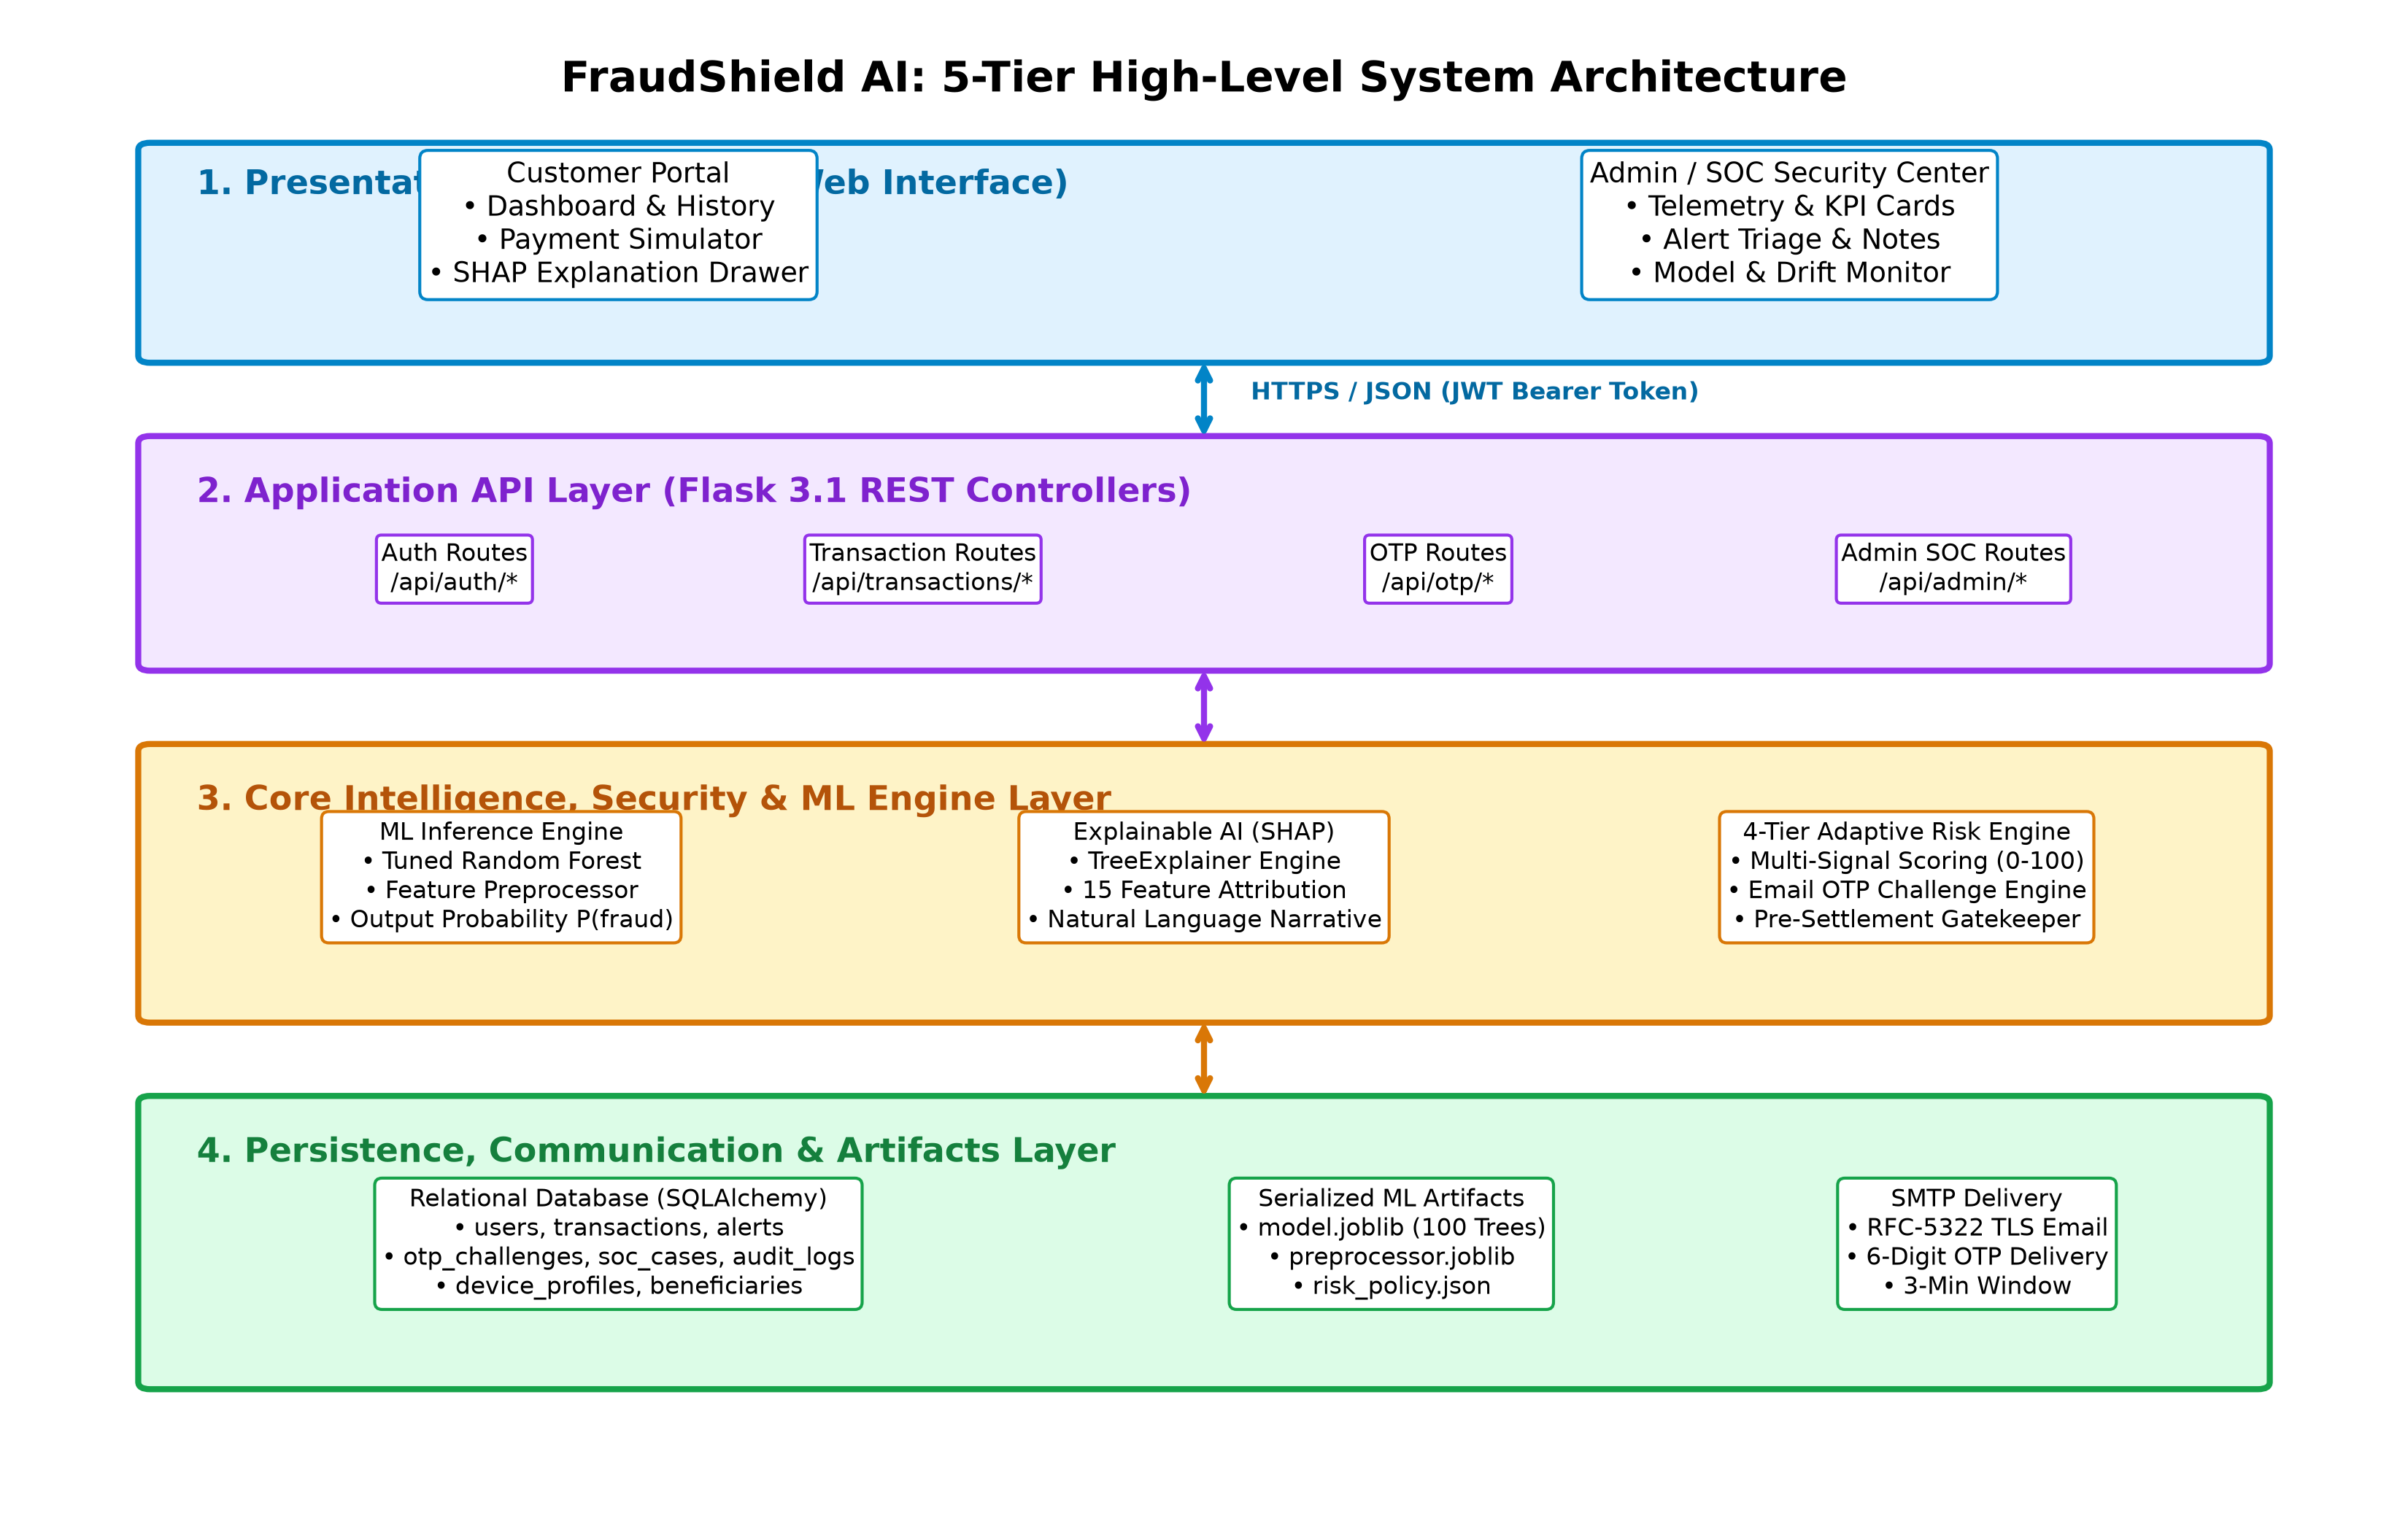
\includegraphics[width=0.92\textwidth]{figures/architecture_diagram.png}
    \caption{FraudShield AI: 5-Tier High-Level System Architecture}
    \label{fig:architecture_diagram}
\end{figure}

The architectural layers operate as follows:
\begin{enumerate}[label=\arabic*.]
    \item \textbf{Presentation Layer}: Delivers responsive client interfaces for both retail customers (payment simulator, dashboard, SHAP drawer) and SOC security officers (alert triage, KPIs, feature drift telemetry).
    \item \textbf{Application API Layer}: Exposes RESTful HTTP endpoints organized into Flask Blueprints (\texttt{auth\_routes}, \texttt{transaction\_routes}, \texttt{otp\_routes}, \texttt{admin\_routes}).
    \item \textbf{Business Logic \& Security Layer}: Implements core domain logic, PIN validation, beneficiary management, and rate limiting.
    \item \textbf{Machine Learning \& Explainability Layer}: Houses the serialized Random Forest model, feature engineering transforms, and the SHAP TreeExplainer.
    \item \textbf{Persistence \& Artifacts Layer}: Manages relational database storage (SQLAlchemy) and physical ML joblib artifacts.
\end{enumerate}

\section{End-to-End System Transaction Workflow}
The transaction lifecycle follows a strict sequence to ensure that fraud detection occurs \textbf{prior} to any financial settlement:

\begin{figure}[htbp]
    \centering
    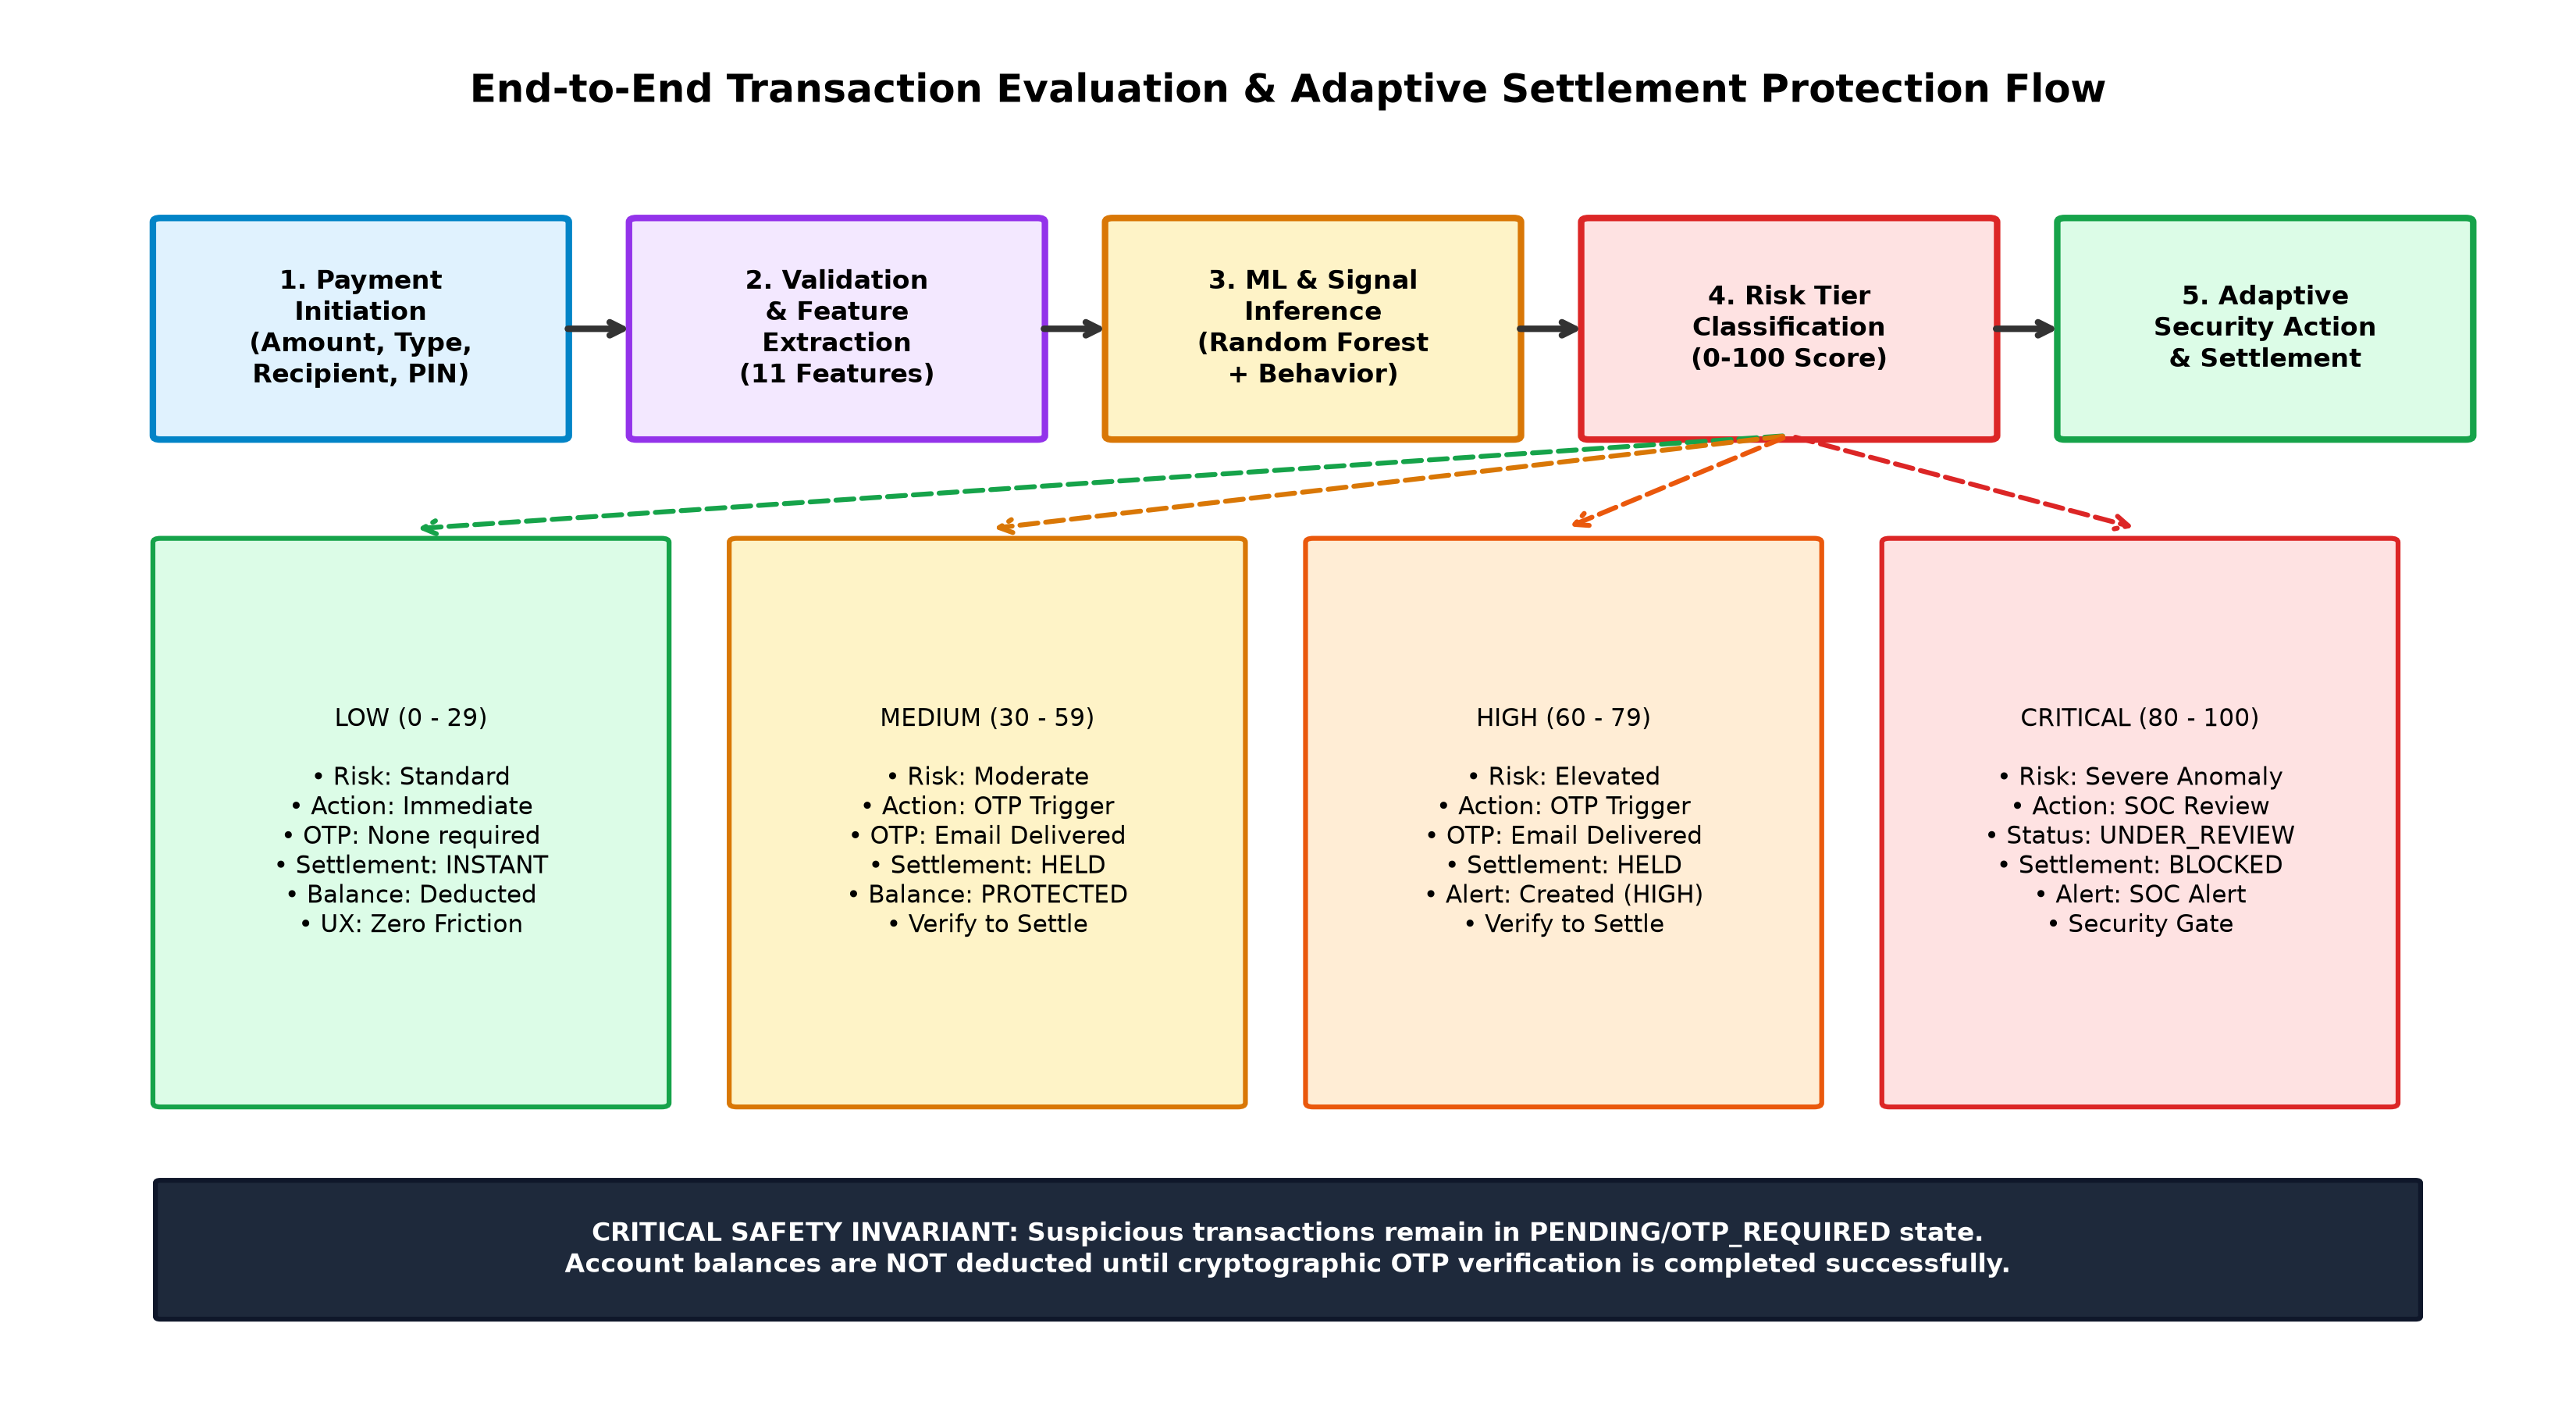
\includegraphics[width=0.95\textwidth]{figures/risk_workflow_diagram.png}
    \caption{End-to-End Transaction Evaluation and Adaptive Settlement Protection Workflow}
    \label{fig:risk_workflow_diagram}
\end{figure}

The chronological execution steps are:
\begin{enumerate}[label=\textbf{Step \arabic*:}]
    \item \textbf{Transaction Initiation}: Customer submits payment payload (recipient VPA/phone, amount, transfer type, 4--6 digit numeric PIN) via the web interface.
    \item \textbf{Authentication \& Account Validation}: Backend verifies active JWT token, validates PIN against stored cryptographic hash, checks account lockout counters, and confirms sufficient balance.
    \item \textbf{Feature Engineering}: Extracts 11 logical transaction properties and computes engineered behavioral indicators:
    \begin{align}
        \text{errorBalanceOrig} &= \text{oldbalanceOrg} - \text{newbalanceOrig} - \text{amount} \\
        \text{errorBalanceDest} &= \text{oldbalanceDest} + \text{amount} - \text{newbalanceDest} \\
        \text{amountToBalanceRatio} &= \frac{\text{amount}}{\text{oldbalanceOrg} + 1.0} \\
        \text{hourOfDay} &= \text{step} \pmod{24}
    \end{align}
    \item \textbf{ML Inference \& SHAP Attribution}: Model preprocessor transforms features into a 15-dimensional vector; Random Forest computes $P(\text{fraud})$; SHAP calculates exact feature Shapley values.
    \item \textbf{4-Tier Risk Classification}: System calculates combined risk score ($0-100$) and assigns risk tier (\textit{LOW, MEDIUM, HIGH, CRITICAL}).
    \item \textbf{Adaptive Security Action}:
    \begin{itemize}
        \item \textit{LOW ($0-29$)}: Instantly approved; sender balance deducted; recipient credited; status \texttt{APPROVED}.
        \item \textit{MEDIUM ($30-59$)}: Held in \texttt{OTP\_REQUIRED}; zero balance deducted; 6-digit Email OTP delivered.
        \item \textit{HIGH ($60-79$)}: Held in \texttt{OTP\_REQUIRED}; zero balance deducted; Email OTP delivered; security alert opened.
        \item \textit{CRITICAL ($80-100$)}: Routed to \texttt{UNDER\_REVIEW}; balance locked; SOC security case opened.
    \end{itemize}
    \item \textbf{OTP Verification \& Final Settlement}: Upon entering valid Email OTP within 180 seconds, atomic settlement executes, updating balances and marking the transaction \texttt{SETTLED}.
\end{enumerate}

\section{Data Flow Diagrams (DFD)}

\subsection{DFD Level 0 — Context Diagram}
Figure~\ref{fig:dfd_level0} illustrates the Level 0 Context Diagram representing external entities interacting with the core platform boundaries.

\begin{figure}[htbp]
    \centering
    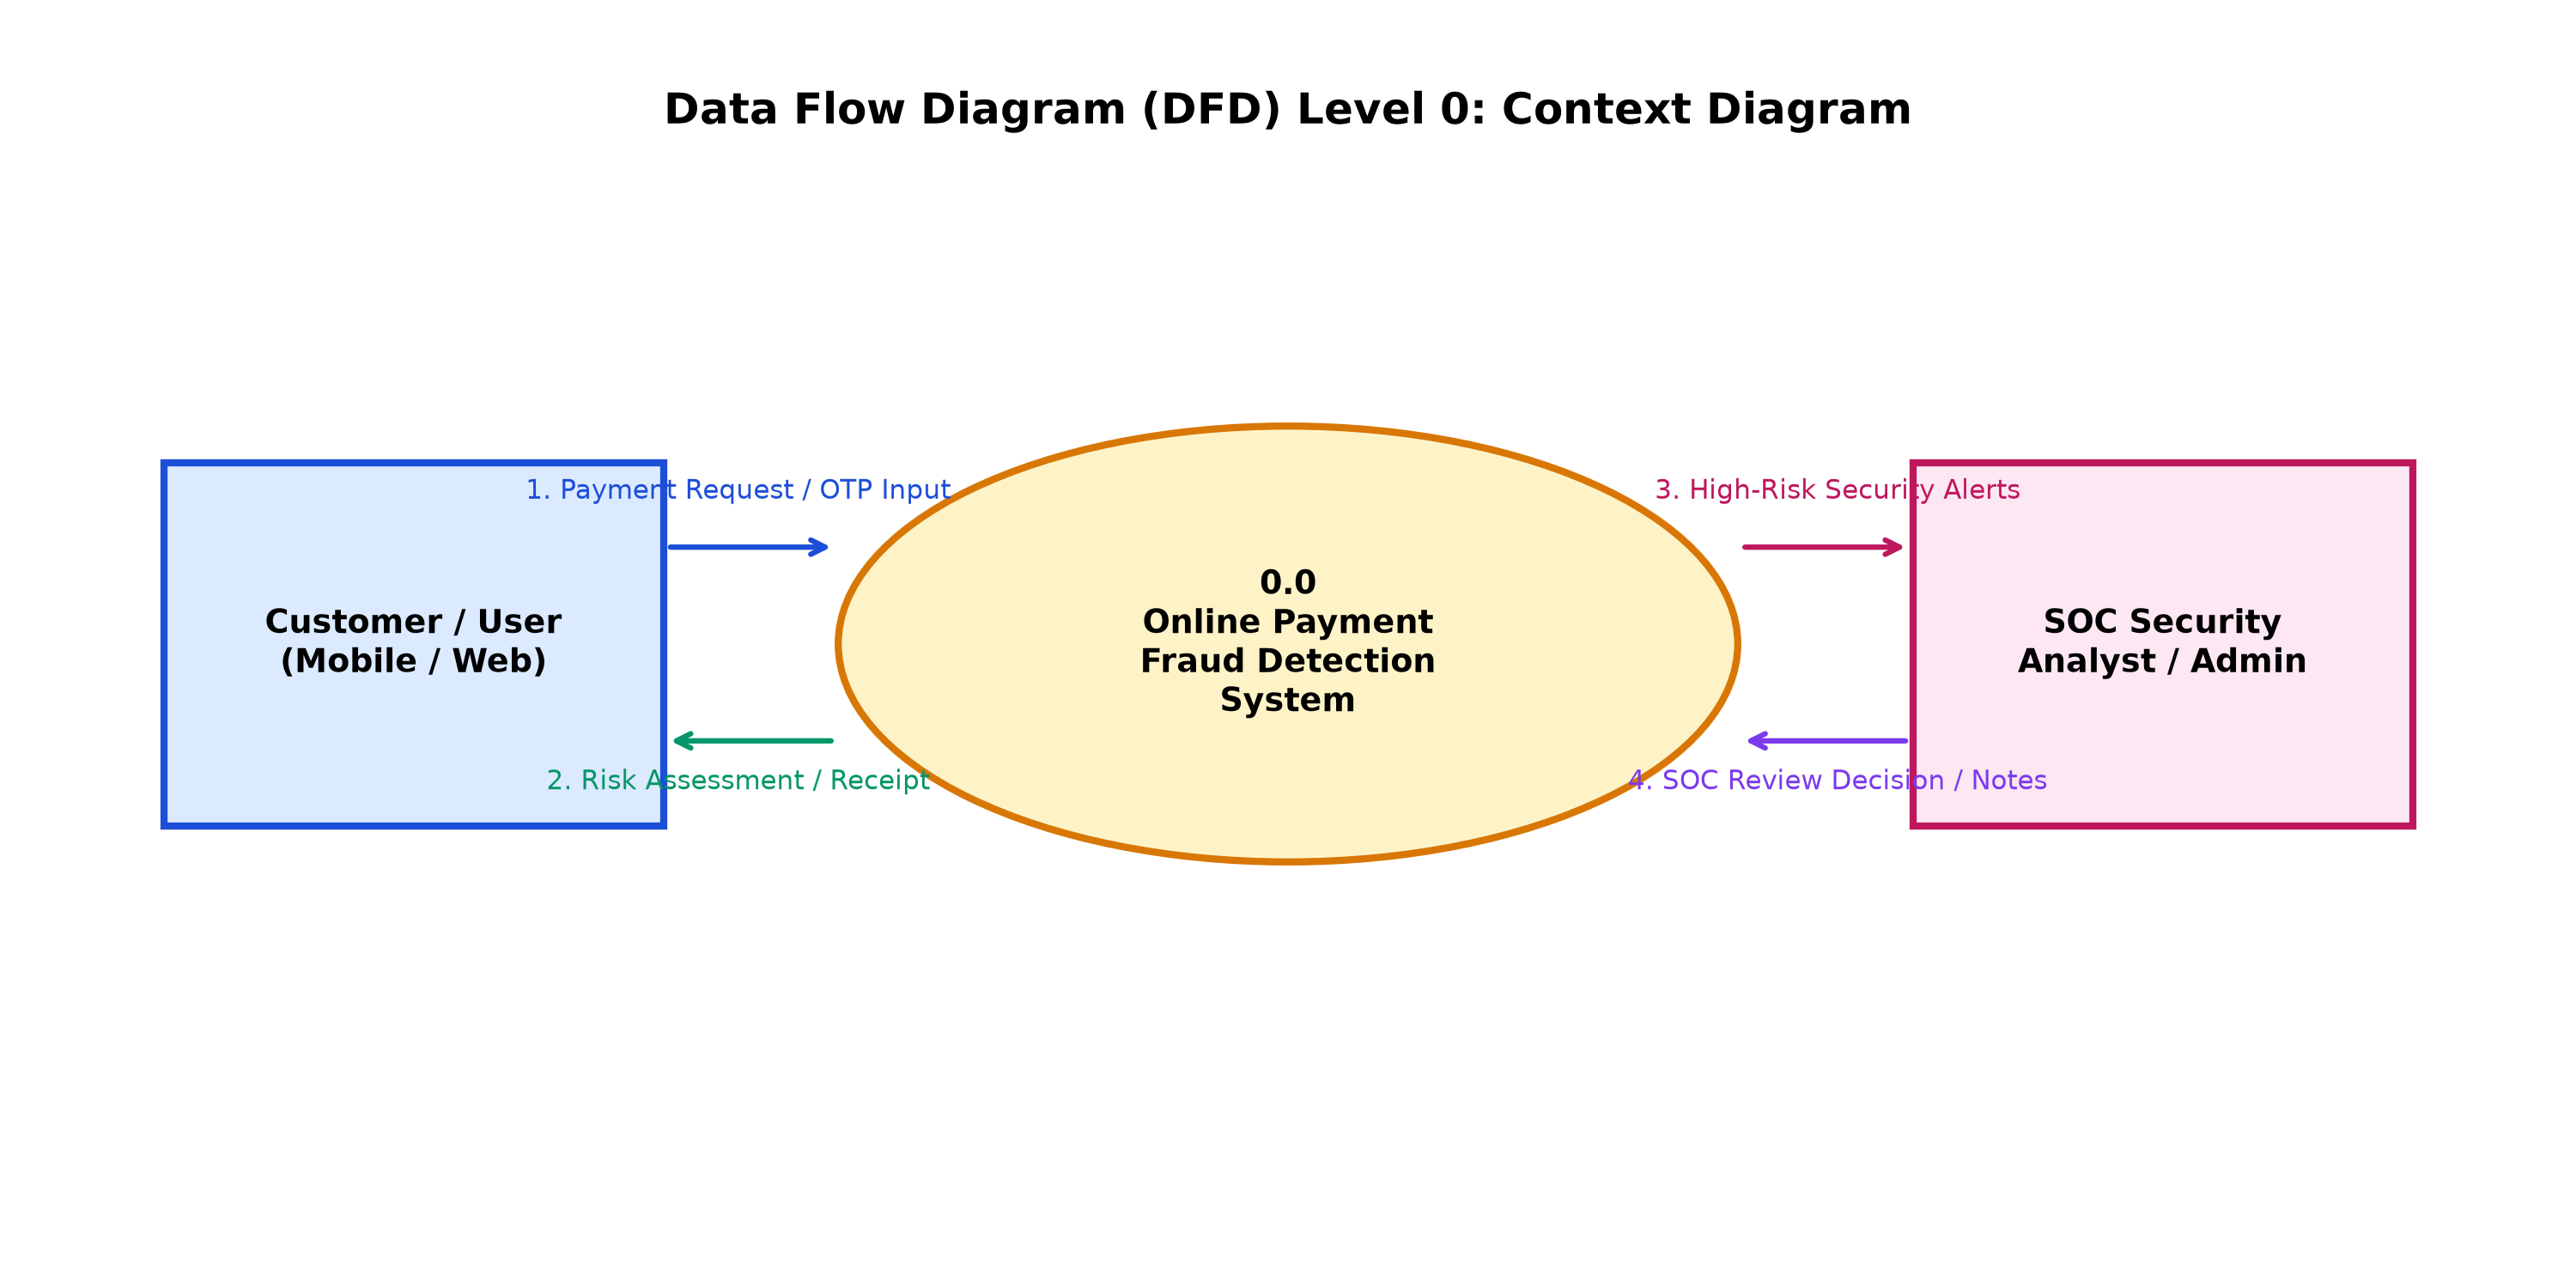
\includegraphics[width=0.85\textwidth]{figures/dfd_level0.png}
    \caption{DFD Level 0: System Context Diagram}
    \label{fig:dfd_level0}
\end{figure}

\subsection{DFD Level 1 — Subsystem Data Flow Diagram}
Figure~\ref{fig:dfd_level1} details the Level 1 functional processes, data stores (D1: Relational Database, D2: ML Artifacts), and data flow pathways across subsystems.

\begin{figure}[htbp]
    \centering
    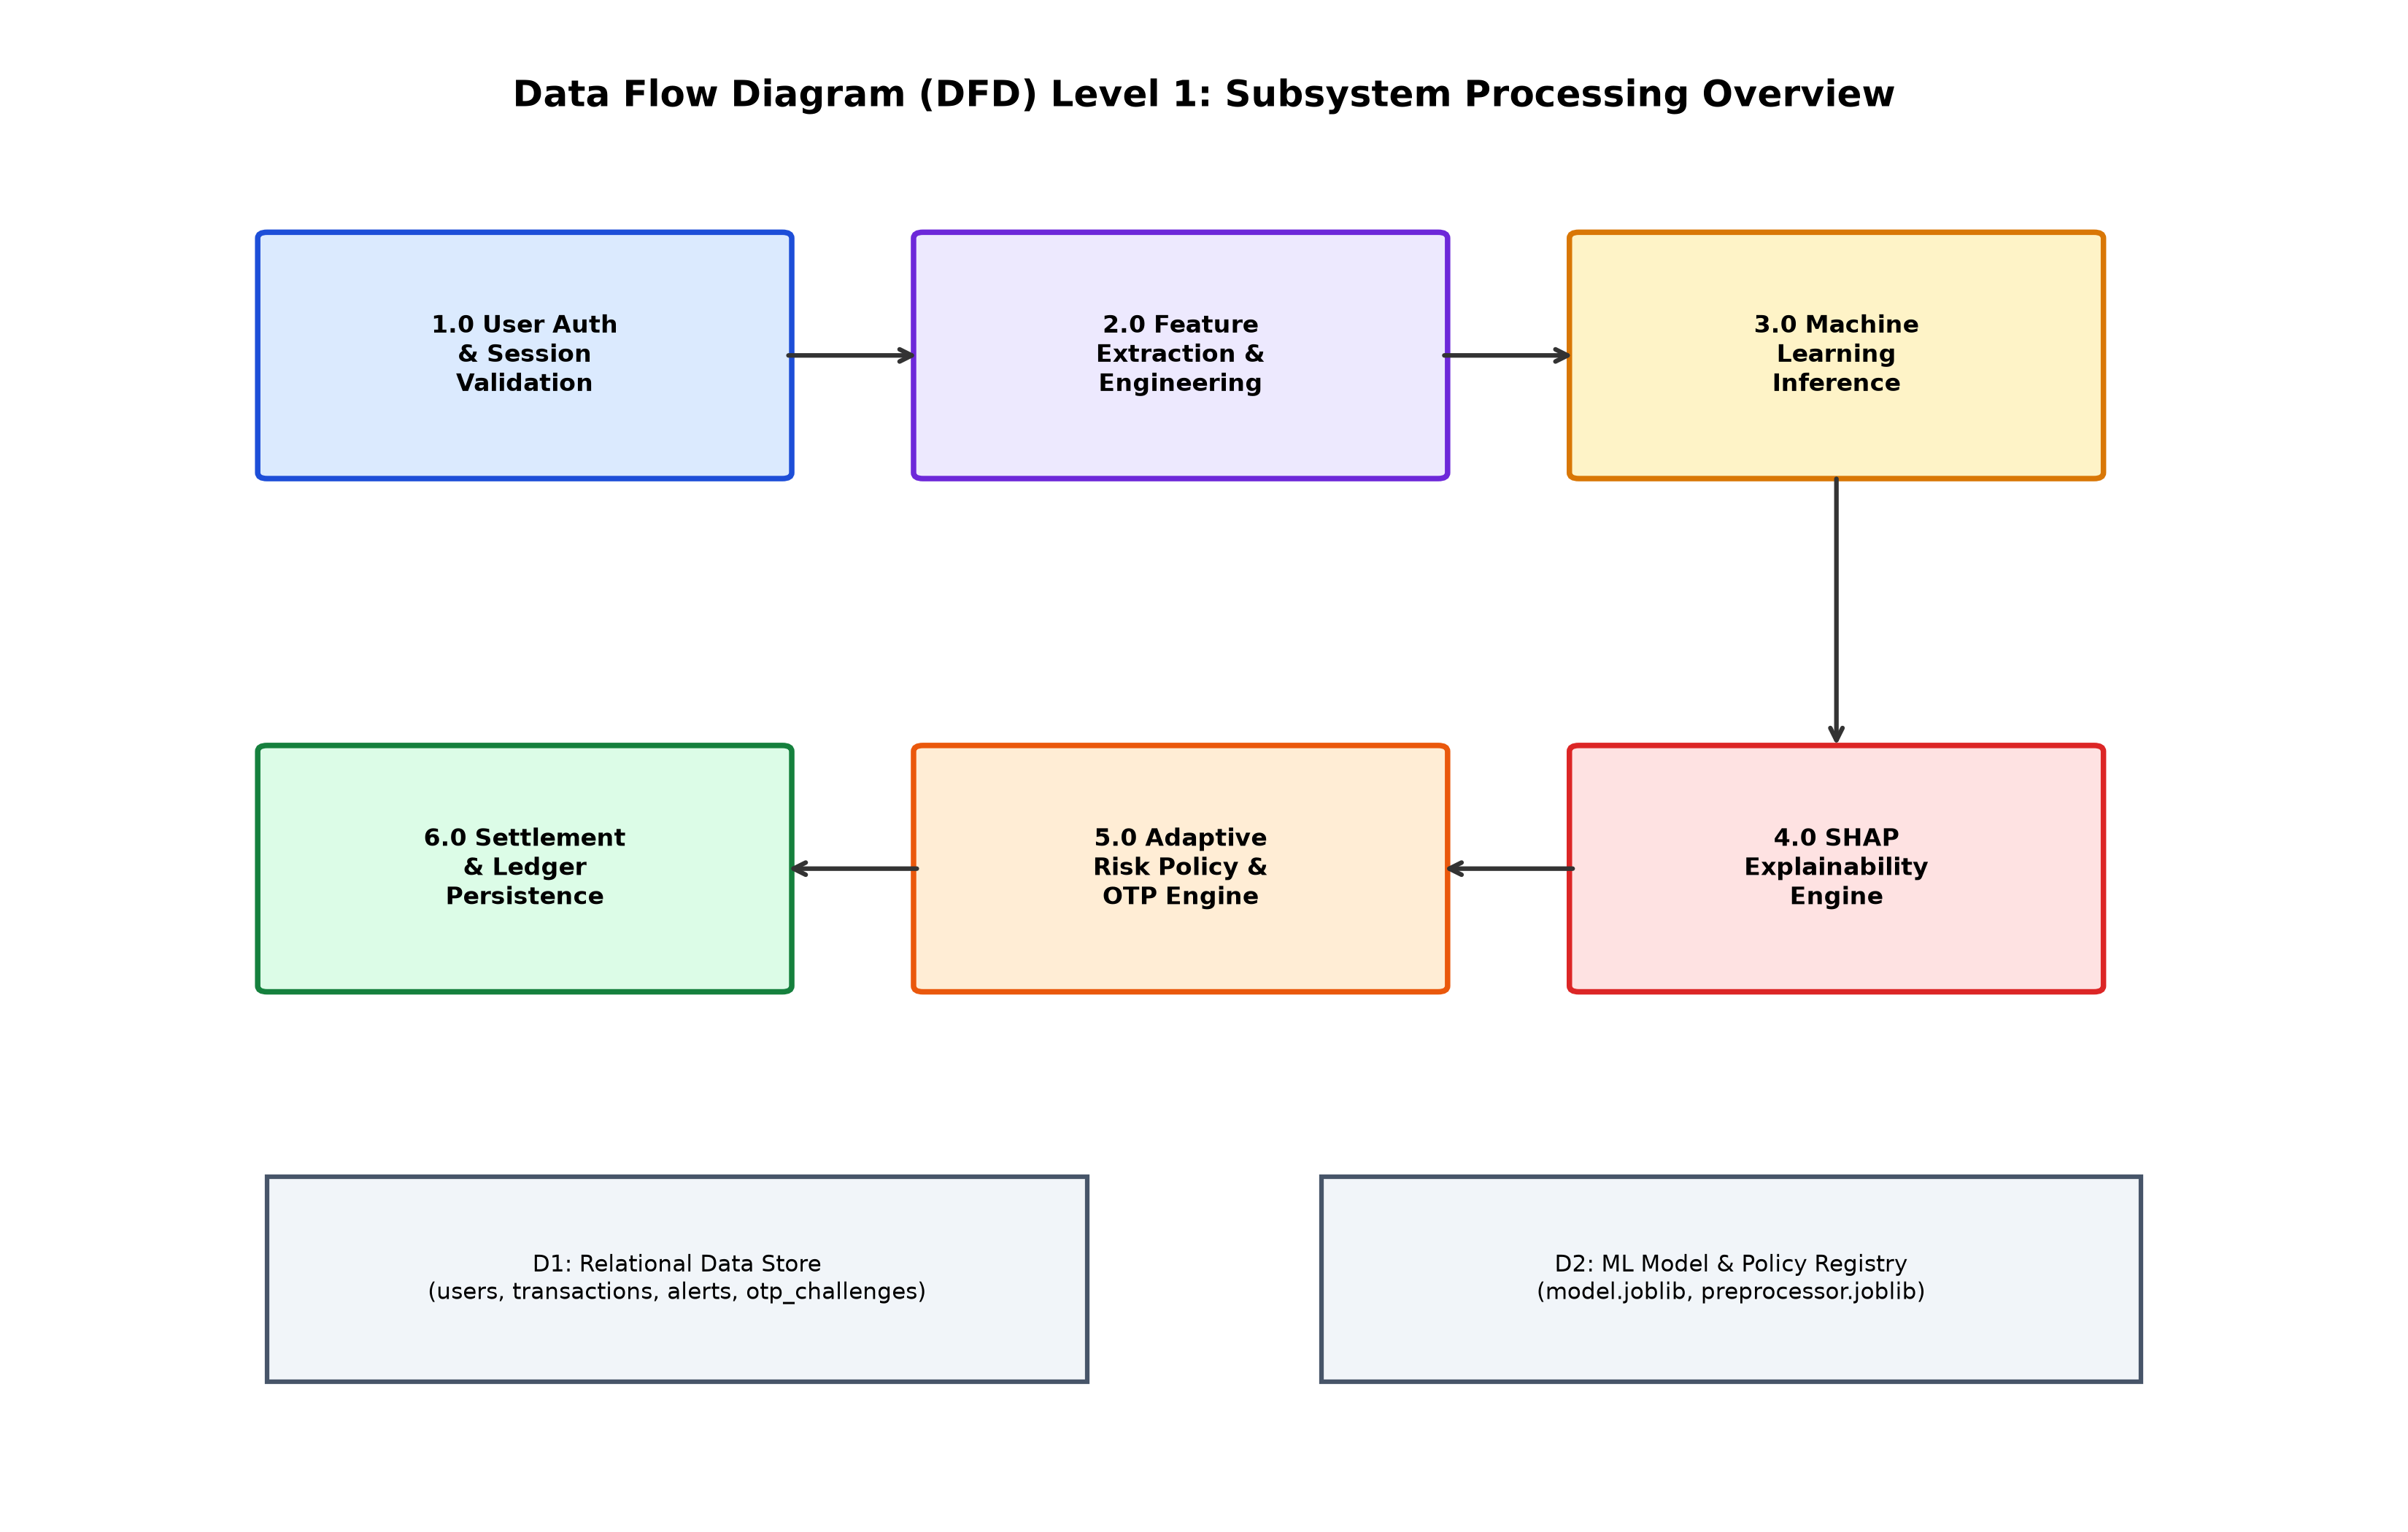
\includegraphics[width=0.88\textwidth]{figures/dfd_level1.png}
    \caption{DFD Level 1: Subsystem Processing Data Flow Diagram}
    \label{fig:dfd_level1}
\end{figure}

\subsection{DFD Level 2 — ML Inference \& Risk Decision Sub-Process}
At Level 2, raw incoming transaction dictionaries are piped through feature sanitization, categorical one-hot encoding, model probability estimation, SHAP attribution decomposition, and policy threshold evaluation, producing the final standardized response payload.

% =========================================================
% CHAPTER 9: DATABASE DESIGN
% =========================================================
\chapter{Database Design}
\label{chap:database_design}

\section{Database Architecture Overview}
The persistence layer of FraudShield AI is implemented using relational database technologies managed through \textbf{SQLAlchemy 2.0 ORM} and \textbf{Flask-Migrate (Alembic)}. The schema is engineered to guarantee strict referential integrity, atomic financial operations, idempotent migrations, and auditability.

\section{Entity Relationship Diagram (ERD)}
Figure~\ref{fig:erd_diagram} depicts the core relational entities, cardinalities, primary keys, and foreign key relationships.

\begin{figure}[htbp]
    \centering
    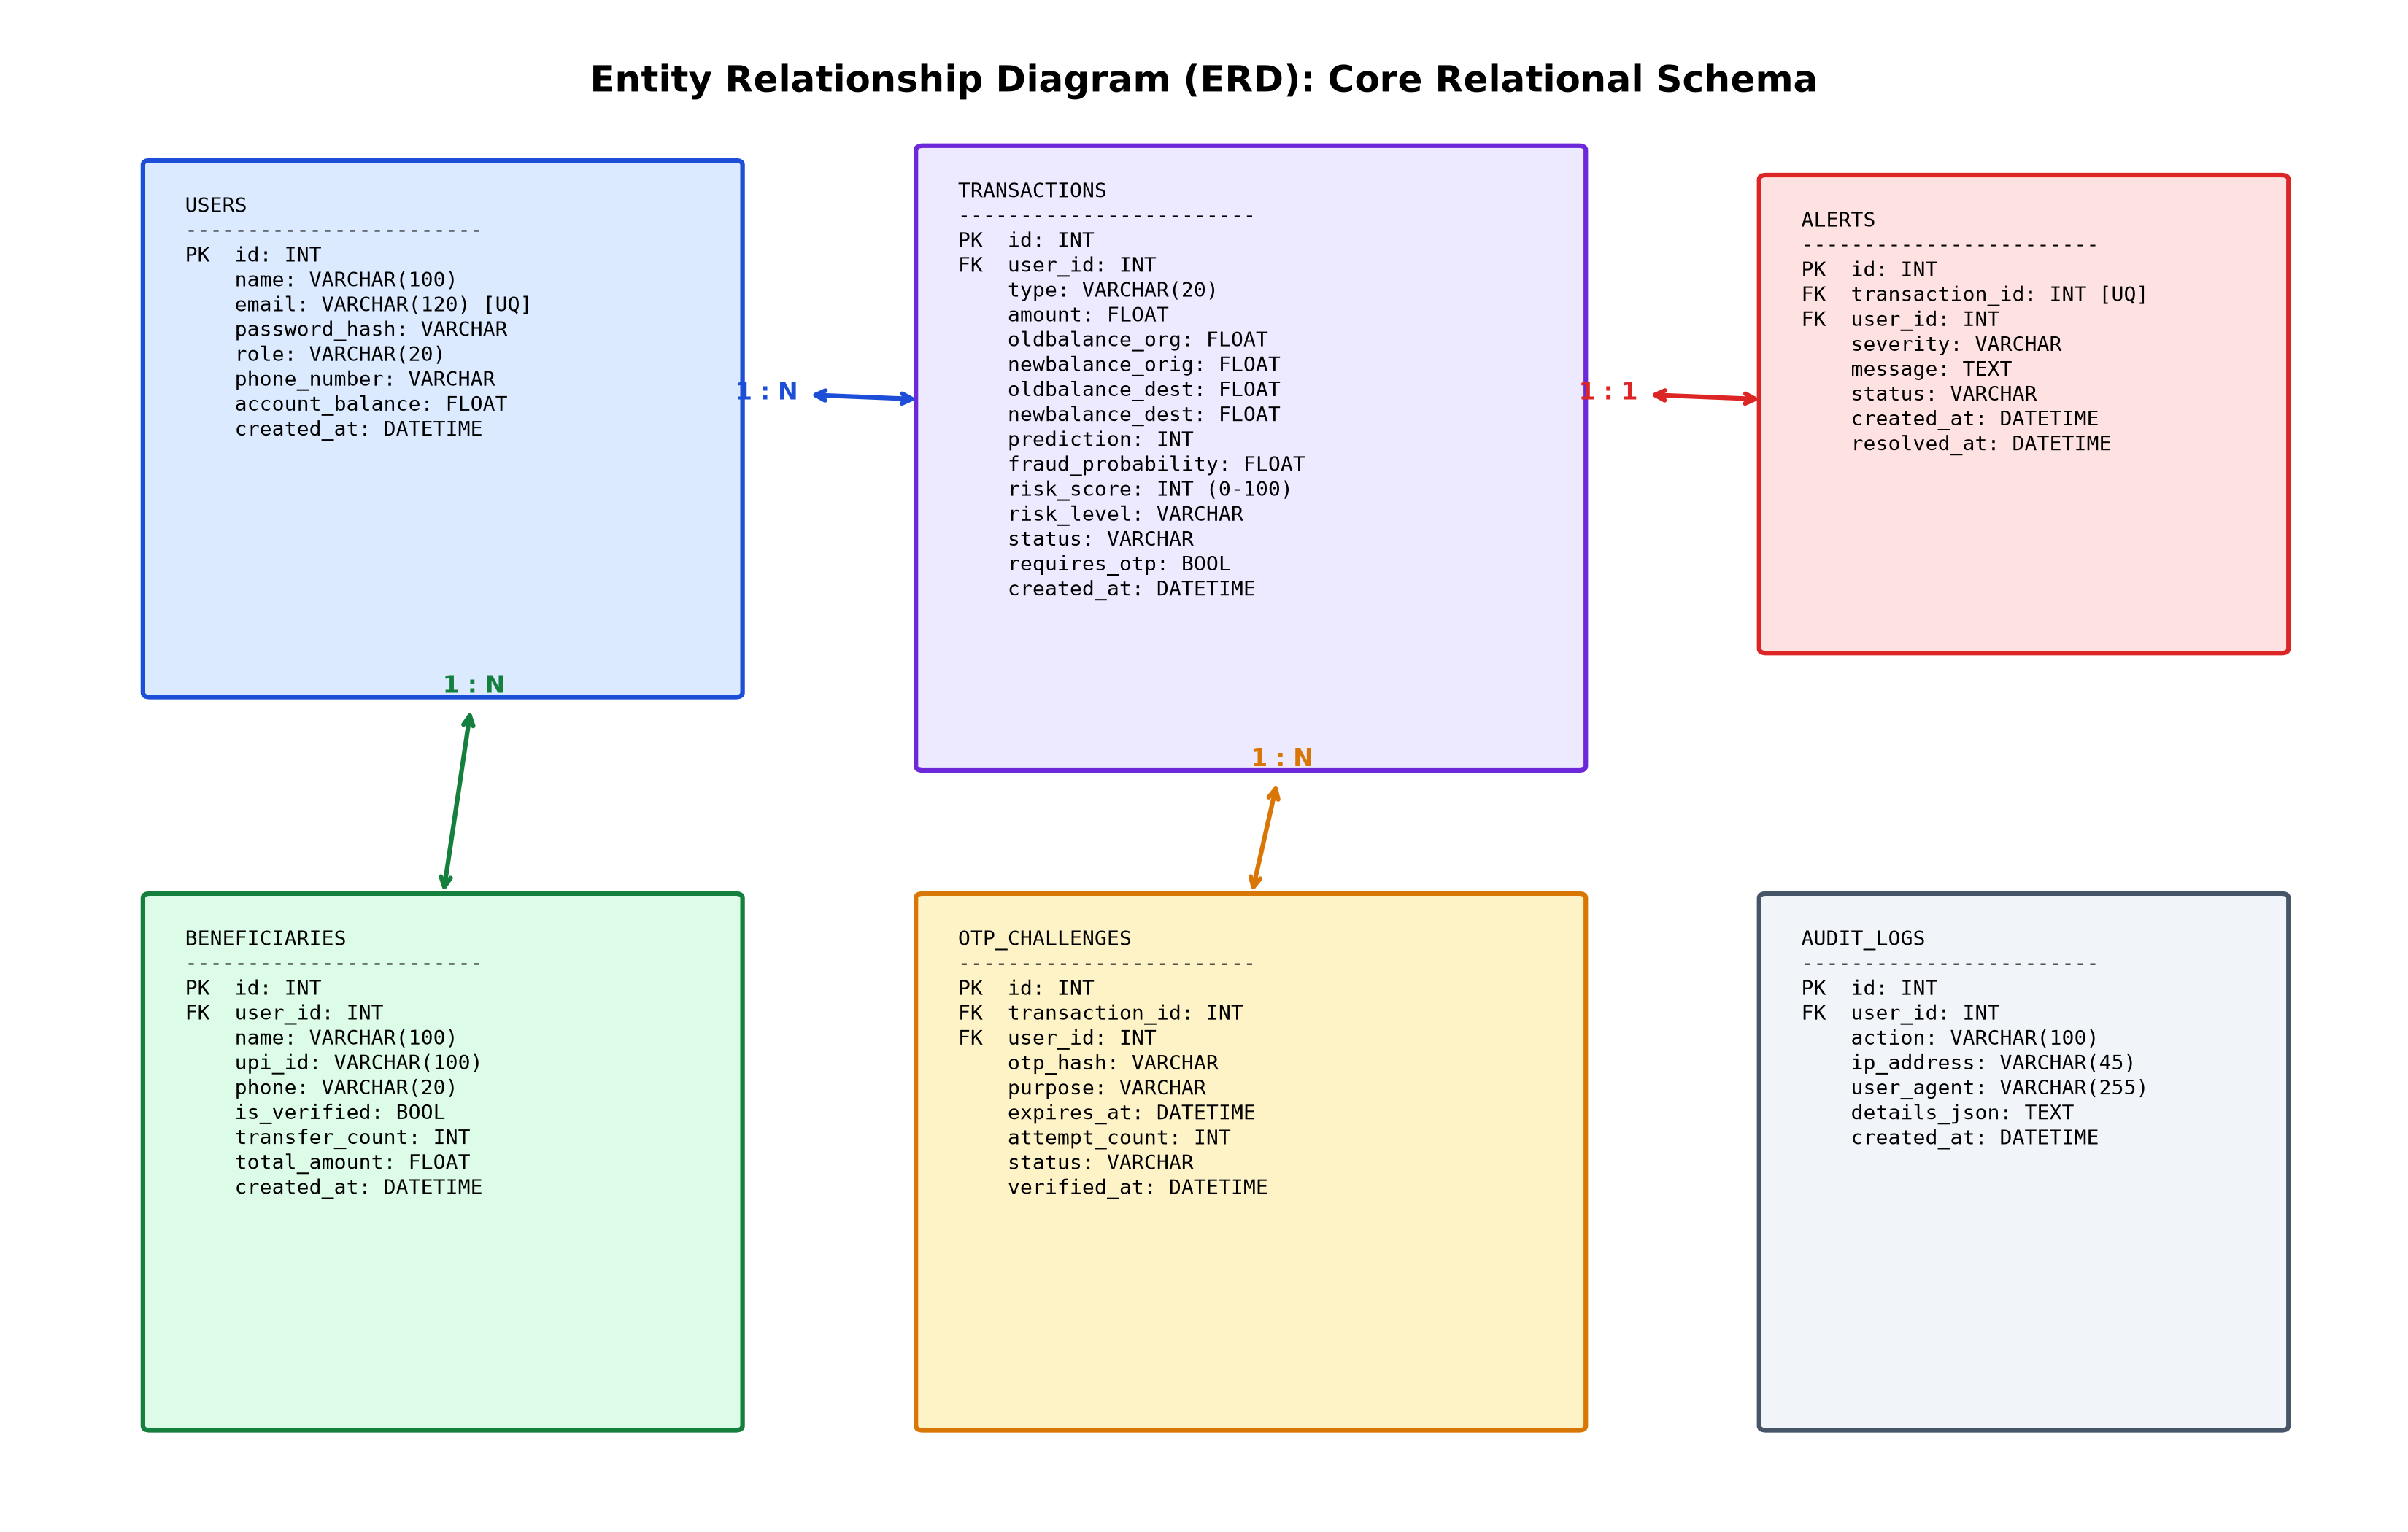
\includegraphics[width=0.92\textwidth]{figures/erd_diagram.png}
    \caption{Entity Relationship Diagram (ERD) of Core Relational Schema}
    \label{fig:erd_diagram}
\end{figure}

\section{Detailed Table Schemas and Constraints}

\subsection{1. \texttt{users} Table}
Stores customer and administrator identities, cryptographic credentials, VPA mappings, and account balances.

\begin{table}[h]
\centering
\caption{Database Schema: \texttt{users} Table}
\label{tab:users_schema}
\begin{tabularx}{\textwidth}{lp{2.8cm}p{1.8cm}X}
\toprule
\textbf{Column Name} & \textbf{Data Type} & \textbf{Nullable} & \textbf{Constraints \& Description} \\
\midrule
\texttt{id} & \texttt{INTEGER} & No & Primary Key, Auto Increment. \\
\texttt{name} & \texttt{VARCHAR(100)} & No & Full customer name. \\
\texttt{email} & \texttt{VARCHAR(120)} & No & Unique, Indexed (\texttt{ix\_users\_email}). \\
\texttt{password\_hash} & \texttt{VARCHAR(255)} & No & Salted PBKDF2/Scrypt hash. \\
\texttt{role} & \texttt{VARCHAR(20)} & No & Check: \texttt{USER} or \texttt{ADMIN}. \\
\texttt{pin\_hash} & \texttt{VARCHAR(255)} & Yes & Salted 4--6 digit numeric PIN hash. \\
\texttt{account\_balance} & \texttt{FLOAT} & No & Default: 100000.0, Check: $\ge 0.0$. \\
\texttt{primary\_upi\_id} & \texttt{VARCHAR(100)} & Yes & Virtual Payment Address (\texttt{user@fraudshield}). \\
\texttt{is\_phone\_verified} & \texttt{BOOLEAN} & No & Default: False. \\
\texttt{created\_at} & \texttt{DATETIME} & No & Indexed account creation timestamp. \\
\bottomrule
\end{tabularx}
\end{table}

\subsection{2. \texttt{transactions} Table}
Maintains the complete financial transaction ledger, ML predictions, risk scores, and serialized SHAP audit payloads.

\begin{table}[h]
\centering
\caption{Database Schema: \texttt{transactions} Table}
\label{tab:transactions_schema}
\begin{tabularx}{\textwidth}{lp{2.8cm}p{1.8cm}X}
\toprule
\textbf{Column Name} & \textbf{Data Type} & \textbf{Nullable} & \textbf{Constraints \& Description} \\
\midrule
\texttt{id} & \texttt{INTEGER} & No & Primary Key, Auto Increment. \\
\texttt{user\_id} & \texttt{INTEGER} & No & Foreign Key $\to$ \texttt{users.id} (On Delete Cascade). \\
\texttt{type} & \texttt{VARCHAR(20)} & No & Payment type (\texttt{TRANSFER}, \texttt{PAYMENT}, etc.). \\
\texttt{amount} & \texttt{FLOAT} & No & Check: \texttt{amount > 0}. \\
\texttt{oldbalance\_org} & \texttt{FLOAT} & No & Sender initial balance prior to transfer. \\
\texttt{newbalance\_orig} & \texttt{FLOAT} & No & Sender final balance after transfer. \\
\texttt{oldbalance\_dest}& \texttt{FLOAT} & No & Recipient initial balance. \\
\texttt{newbalance\_dest}& \texttt{FLOAT} & No & Recipient final balance. \\
\texttt{prediction} & \texttt{INTEGER} & No & Binary ML prediction ($0$ or $1$), Indexed. \\
\texttt{fraud\_probability}& \texttt{FLOAT} & No & Continuous probability $P(\text{fraud}) \in [0.0, 1.0]$. \\
\texttt{risk\_score} & \texttt{INTEGER} & No & Standardized risk score ($0-100$), Indexed. \\
\texttt{risk\_level} & \texttt{VARCHAR(20)} & No & Check: \texttt{LOW}, \texttt{MEDIUM}, \texttt{HIGH}, \texttt{CRITICAL}. \\
\texttt{status} & \texttt{VARCHAR(30)} & No & Status: \texttt{APPROVED}, \texttt{OTP\_REQUIRED}, \texttt{UNDER\_REVIEW}. \\
\texttt{requires\_otp} & \texttt{BOOLEAN} & No & Multi-factor challenge requirement flag. \\
\texttt{explanation\_json}& \texttt{TEXT} & Yes & JSON-serialized SHAP feature attributions. \\
\texttt{created\_at} & \texttt{DATETIME} & No & Compound Index (\texttt{user\_id}, \texttt{created\_at}). \\
\bottomrule
\end{tabularx}
\end{table}

\subsection{3. \texttt{alerts} Table}
Maintains high-priority security incident records generated automatically for SOC investigation.

\begin{table}[h]
\centering
\caption{Database Schema: \texttt{alerts} Table}
\label{tab:alerts_schema}
\begin{tabularx}{\textwidth}{lp{2.8cm}p{1.8cm}X}
\toprule
\textbf{Column Name} & \textbf{Data Type} & \textbf{Nullable} & \textbf{Constraints \& Description} \\
\midrule
\texttt{id} & \texttt{INTEGER} & No & Primary Key, Auto Increment. \\
\texttt{transaction\_id} & \texttt{INTEGER} & No & Foreign Key $\to$ \texttt{transactions.id} (Unique). \\
\texttt{user\_id} & \texttt{INTEGER} & No & Foreign Key $\to$ \texttt{users.id} (On Delete Cascade). \\
\texttt{severity} & \texttt{VARCHAR(20)} & No & Check: \texttt{MEDIUM}, \texttt{HIGH}, \texttt{CRITICAL}. \\
\texttt{message} & \texttt{TEXT} & No & Grounded explanation narrative. \\
\texttt{status} & \texttt{VARCHAR(20)} & No & Check: \texttt{OPEN}, \texttt{RESOLVED}, \texttt{DISMISSED}. \\
\texttt{created\_at} & \texttt{DATETIME} & No & Incident generation timestamp. \\
\texttt{resolved\_at} & \texttt{DATETIME} & Yes & Resolution timestamp. \\
\bottomrule
\end{tabularx}
\end{table}

\subsection{4. \texttt{otp\_challenges} Table}
Stores hashed one-time verification tokens, expiration timestamps, attempt counters, and verification state.

\begin{table}[h]
\centering
\caption{Database Schema: \texttt{otp\_challenges} Table}
\label{tab:otp_challenges_schema}
\begin{tabularx}{\textwidth}{lp{2.8cm}p{1.8cm}X}
\toprule
\textbf{Column Name} & \textbf{Data Type} & \textbf{Nullable} & \textbf{Constraints \& Description} \\
\midrule
\texttt{id} & \texttt{INTEGER} & No & Primary Key, Auto Increment. \\
\texttt{transaction\_id} & \texttt{INTEGER} & No & Foreign Key $\to$ \texttt{transactions.id}. \\
\texttt{user\_id} & \texttt{INTEGER} & No & Foreign Key $\to$ \texttt{users.id}. \\
\texttt{otp\_hash} & \texttt{VARCHAR(255)} & No & Salted PBKDF2 hash of 6-digit OTP code. \\
\texttt{expires\_at} & \texttt{DATETIME} & No & Expiration timestamp (180-second TTL). \\
\texttt{attempt\_count} & \texttt{INTEGER} & No & Default: 0, Max allowed: 3. \\
\texttt{status} & \texttt{VARCHAR(20)} & No & Check: \texttt{ACTIVE}, \texttt{VERIFIED}, \texttt{EXPIRED}, \texttt{EXHAUSTED}. \\
\texttt{verified\_at} & \texttt{DATETIME} & Yes & Successful verification timestamp. \\
\bottomrule
\end{tabularx}
\end{table}

\section{Essential SQL Query Patterns}
\subsection{Atomic Settlement Execution (Double-Debit Protection)}
\begin{lstlisting}[language=SQL, caption={Atomic Settlement and Balance Deduction Query}]
BEGIN TRANSACTION;
-- 1. Deduct amount from sender account
UPDATE users 
SET account_balance = account_balance - :tx_amount 
WHERE id = :sender_id AND account_balance >= :tx_amount;

-- 2. Update transaction status to SETTLED
UPDATE transactions 
SET status = 'APPROVED', decision = 'SETTLED_AFTER_OTP' 
WHERE id = :tx_id AND status = 'OTP_REQUIRED';

-- 3. Mark OTP challenge as verified
UPDATE otp_challenges 
SET status = 'VERIFIED', verified_at = CURRENT_TIMESTAMP 
WHERE id = :challenge_id AND status = 'ACTIVE';
COMMIT;
\end{lstlisting}

\subsection{SOC Incident Triage Query}
\begin{lstlisting}[language=SQL, caption={SOC Open High-Risk Alerts Retrieval Query}]
SELECT a.id, a.severity, a.message, t.amount, t.risk_score, u.email, a.created_at
FROM alerts a
JOIN transactions t ON a.transaction_id = t.id
JOIN users u ON a.user_id = u.id
WHERE a.status = 'OPEN'
ORDER BY t.risk_score DESC, a.created_at DESC;
\end{lstlisting}

% =========================================================
% CHAPTER 10: MODULE DESCRIPTION
% =========================================================
\chapter{Module Description}
\label{chap:modules}

\section{Module Architecture Overview}
FraudShield AI is organized into nine discrete, decoupled functional modules. Each module encapsulates specific domain logic, communicates via structured Python service contracts, and interacts with persistent data stores through SQLAlchemy ORM.

% ---------------------------------------------------------
\section{Module 1: Authentication \& Identity Management}
\begin{itemize}
    \item \textbf{Purpose}: Handles user registration, cryptographically secure password hashing, JWT token issuance, and password recovery.
    \item \textbf{Inputs}: Registration payload (\texttt{name}, \texttt{email}, \texttt{password}, \texttt{role}) or login credentials.
    \item \textbf{Processing}: Hashes passwords via salted PBKDF2/Scrypt; enforces anti-enumeration timing; issues signed 24-hour JWT access tokens.
    \item \textbf{Outputs}: Signed JWT Bearer token and sanitized user profile dictionary.
    \item \textbf{Database Interaction}: Read/Write on \texttt{users} and \texttt{password\_reset\_tokens}.
    \item \textbf{Related APIs}: \texttt{POST /api/auth/register}, \texttt{POST /api/auth/login}, \texttt{POST /api/auth/forgot-password}.
    \item \textbf{Security Considerations}: Password hashes excluded from serialization; brute-force protection with account locking.
    \item \textbf{Related Test Cases}: \texttt{test\_auth.py}, \texttt{test\_password\_reset.py}.
\end{itemize}

% ---------------------------------------------------------
\section{Module 2: Payment \& Transaction Simulation}
\begin{itemize}
    \item \textbf{Purpose}: Accepts payment requests (UPI, P2P, VPA, Merchant QR), verifies Payment PIN, and manages transaction state transitions.
    \item \textbf{Inputs}: Payment payload (\texttt{amount}, \texttt{type}, \texttt{beneficiary\_id} or recipient VPA/phone, \texttt{payment\_pin}).
    \item \textbf{Processing}: Verifies 4--6 digit numeric PIN; verifies sender balance; triggers feature extraction and risk assessment; blocks balance deduction if flagged.
    \item \textbf{Outputs}: Initial transaction status (\texttt{APPROVED}, \texttt{OTP\_REQUIRED}, or \texttt{UNDER\_REVIEW}).
    \item \textbf{Database Interaction}: Read/Write on \texttt{transactions} and \texttt{users}.
    \item \textbf{Related APIs}: \texttt{POST /api/transactions/predict}, \texttt{GET /api/transactions/my-history}.
    \item \textbf{Security Considerations}: Account lockout after 3 consecutive failed PIN attempts; double-debit prevention.
    \item \textbf{Related Test Cases}: \texttt{test\_payment\_pin\_flow.py}, \texttt{test\_upi\_payment\_flow.py}.
\end{itemize}

% ---------------------------------------------------------
\section{Module 3: Feature Engineering \& Preprocessing}
\begin{itemize}
    \item \textbf{Purpose}: Sanitizes transaction attributes, removes data-leakage columns, and constructs 15 transformed mathematical features.
    \item \textbf{Inputs}: Raw transaction parameters (\texttt{amount}, \texttt{type}, balances before and after).
    \item \textbf{Processing}: Computes \texttt{errorBalanceOrig}, \texttt{errorBalanceDest}, \texttt{amountToBalanceRatio}, \texttt{hourOfDay}, and applies \texttt{ColumnTransformer} one-hot encoding.
    \item \textbf{Outputs}: 15-dimensional numeric numpy array ready for model inference.
    \item \textbf{Database Interaction}: Stateless (in-memory execution).
    \item \textbf{Related APIs}: Internal service method (\texttt{engineer\_features()}).
    \item \textbf{Security Considerations}: Strict exclusion of target leakage columns (\texttt{isFraud}, \texttt{isFlaggedFraud}, raw account IDs).
    \item \textbf{Related Test Cases}: \texttt{test\_feature\_engineering.py}, \texttt{test\_preprocessing.py}.
\end{itemize}

% ---------------------------------------------------------
\section{Module 4: Machine Learning Inference Engine}
\begin{itemize}
    \item \textbf{Purpose}: Evaluates transformed transaction vectors against the trained Random Forest ensemble model.
    \item \textbf{Inputs}: 15-dimensional preprocessed numeric vector.
    \item \textbf{Processing}: Executes \texttt{predict\_proba()} across 100 decision trees; computes continuous fraud probability $P(\text{fraud})$.
    \item \textbf{Outputs}: Continuous probability value $P(\text{fraud}) \in [0.0, 1.0]$ and binary class prediction.
    \item \textbf{Database Interaction}: Reads serialized \texttt{model.joblib} at application startup.
    \item \textbf{Related APIs}: Internal service method (\texttt{InferenceService.predict()}).
    \item \textbf{Security Considerations}: Memory-cached singleton pipeline to prevent disk I/O latency bottlenecks.
    \item \textbf{Related Test Cases}: \texttt{test\_inference.py}, \texttt{test\_strong\_models.py}.
\end{itemize}

% ---------------------------------------------------------
\section{Module 5: Explainable AI (SHAP) Engine}
\begin{itemize}
    \item \textbf{Purpose}: Computes exact Shapley feature attributions and synthesizes human-readable risk narratives.
    \item \textbf{Inputs}: 15-dimensional feature vector and model prediction object.
    \item \textbf{Processing}: Invokes \texttt{shap.TreeExplainer} to calculate Shapley values; maps encoded column indices to human-readable labels; derives top positive and negative risk drivers.
    \item \textbf{Outputs}: Dual-view payload containing top-5 contributing features and natural language narrative.
    \item \textbf{Database Interaction}: Serializes complete explanation dictionary to \texttt{transactions.explanation\_json}.
    \item \textbf{Related APIs}: \texttt{GET /api/transactions/<id>/explanation}.
    \item \textbf{Security Considerations}: Jargon-free presentation for customers; mathematical precision for SOC analysts.
    \item \textbf{Related Test Cases}: \texttt{test\_shap.py}.
\end{itemize}

% ---------------------------------------------------------
\section{Module 6: 4-Tier Adaptive Risk Engine}
\begin{itemize}
    \item \textbf{Purpose}: Combines ML probabilities with behavioral heuristic signals to produce the final $0-100$ risk score and assign routing tiers.
    \item \textbf{Inputs}: ML fraud probability and behavioral telemetry (account draining ratio, transaction frequency).
    \item \textbf{Processing}: Calculates weighted risk score:
    \begin{equation}
        \text{Risk Score} = \text{clamp}\left(\text{round}\left(w_{\text{ml}} \cdot (P(\text{fraud}) \times 100) + w_{\text{signals}} \cdot S_{\text{behavioral}}\right), 0, 100\right)
    \end{equation}
    \item \textbf{Outputs}: Standardized risk score ($0-100$), assigned tier (\textit{LOW, MEDIUM, HIGH, CRITICAL}), and security action directive.
    \item \textbf{Database Interaction}: Read/Write on \texttt{transactions.risk\_score} and \texttt{transactions.risk\_level}.
    \item \textbf{Related APIs}: Internal service method (\texttt{RiskDecisionService.evaluate()}).
    \item \textbf{Security Considerations}: Guarantees deterministic threshold classification.
    \item \textbf{Related Test Cases}: \texttt{test\_risk\_engine.py}, \texttt{test\_hybrid\_risk\_engine.py}.
\end{itemize}

% ---------------------------------------------------------
\section{Module 7: Email OTP Step-Up Verification \& Settlement Guard}
\begin{itemize}
    \item \textbf{Purpose}: Generates, delivers, and validates 6-digit numeric OTP verification challenges for held transactions.
    \item \textbf{Inputs}: Transaction ID, user ID, and candidate 6-digit OTP string.
    \item \textbf{Processing}: Generates cryptographically secure 6-digit code; stores salted PBKDF2 hash; delivers via RFC-5322 SMTP TLS; validates against 180-second TTL and 3-attempt limit; triggers atomic balance deduction on success.
    \item \textbf{Outputs}: Verification confirmation or rejection error.
    \item \textbf{Database Interaction}: Read/Write on \texttt{otp\_challenges}, \texttt{transactions}, and \texttt{users}.
    \item \textbf{Related APIs}: \texttt{POST /api/otp/generate}, \texttt{POST /api/otp/verify}.
    \item \textbf{Security Considerations}: Settlement locked until verification; single-use OTP invalidation; rate-limited attempts.
    \item \textbf{Related Test Cases}: \texttt{test\_email\_otp\_delivery.py}, \texttt{test\_medium\_high\_otp\_stepup.py}.
\end{itemize}

% ---------------------------------------------------------
\section{Module 8: Beneficiary Intelligence}
\begin{itemize}
    \item \textbf{Purpose}: Manages trusted recipient accounts, tracks transfer history, and detects first-time beneficiary anomalies.
    \item \textbf{Inputs}: Beneficiary details (\texttt{name}, \texttt{upi\_id}, \texttt{phone}, \texttt{nickname}).
    \item \textbf{Processing}: Tenant-isolated CRUD operations; calculates recipient trust scores based on historical transaction frequency.
    \item \textbf{Outputs}: Beneficiary list with verification status tags.
    \item \textbf{Database Interaction}: Read/Write on \texttt{beneficiaries}.
    \item \textbf{Related APIs}: \texttt{GET /api/beneficiaries}, \texttt{POST /api/beneficiaries}.
    \item \textbf{Security Considerations}: Strict IDOR checks ensuring users cannot access or modify other users' beneficiaries.
    \item \textbf{Related Test Cases}: \texttt{test\_beneficiary\_intelligence.py}.
\end{itemize}

% ---------------------------------------------------------
\section{Module 9: Security Operations Center (SOC) \& Alert Triage}
\begin{itemize}
    \item \textbf{Purpose}: Provides security officers with real-time incident queues, system KPIs, and model drift telemetry.
    \item \textbf{Inputs}: Analyst filter criteria, investigation notes, and alert resolution codes.
    \item \textbf{Processing}: Computes SQL database aggregations; calculates fraud rates; updates alert status to \texttt{RESOLVED} or \texttt{DISMISSED} with immutable audit logs.
    \item \textbf{Outputs}: Rendered Chart.js telemetry charts, alert triage tables, and resolution receipts.
    \item \textbf{Database Interaction}: Read/Write on \texttt{alerts}, \texttt{soc\_cases}, \texttt{case\_notes}, and \texttt{audit\_logs}.
    \item \textbf{Related APIs}: \texttt{GET /api/admin/overview}, \texttt{GET /api/admin/alerts}, \texttt{POST /api/admin/alerts/<id>/resolve}.
    \item \textbf{Security Considerations}: Protected by strict \texttt{ADMIN} role enforcement.
    \item \textbf{Related Test Cases}: \texttt{test\_admin\_soc.py}, \texttt{test\_soc\_case\_management.py}.
\end{itemize}

% =========================================================
% CHAPTER 11: UML MODELING
% =========================================================
\chapter{UML Modeling}
\label{chap:uml_modeling}

\section{Introduction to System Modeling}
Unified Modeling Language (UML) diagrams provide standardized visual representations of system actors, object interactions, behavioral states, and static architectural structures.

\section{Use Case Diagram}
Figure~\ref{fig:uml_use_case} illustrates the UML Use Case Diagram defining the operational boundaries between regular retail customers and SOC security administrators.

\begin{figure}[htbp]
    \centering
    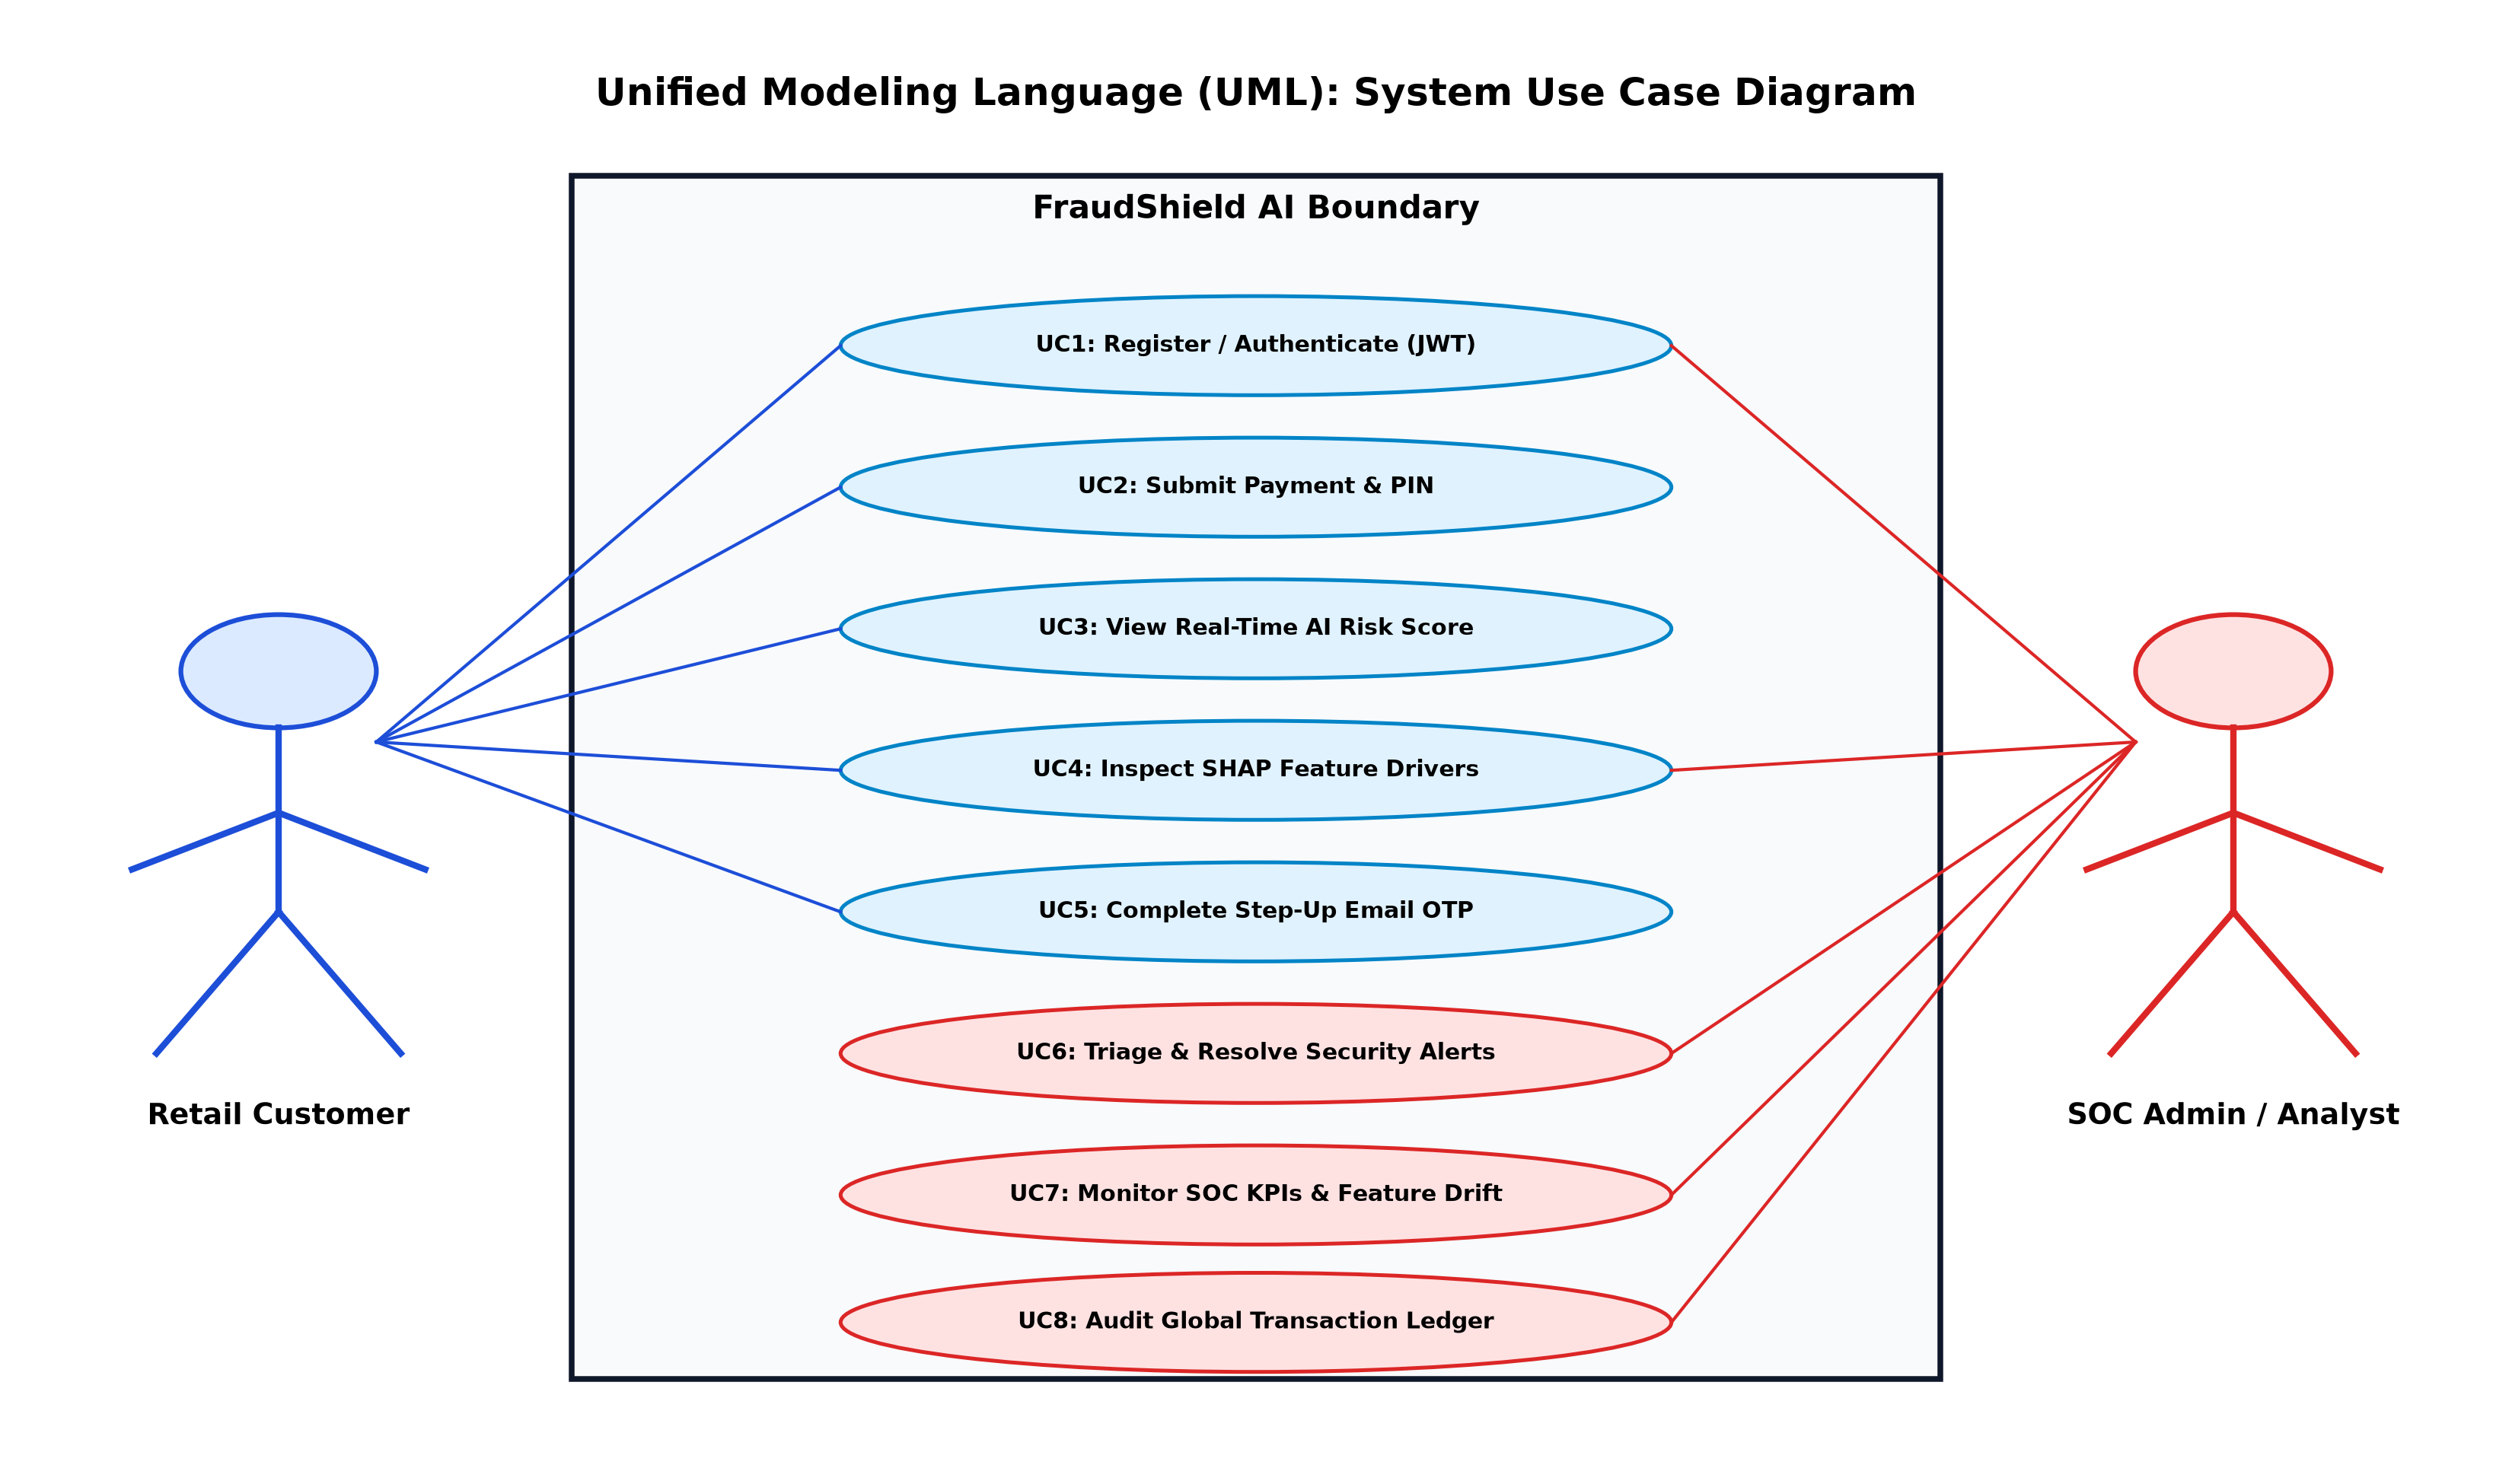
\includegraphics[width=0.95\textwidth]{figures/uml_use_case.png}
    \caption{UML Use Case Diagram: Customer and Administrator Interactions}
    \label{fig:uml_use_case}
\end{figure}

\subsection{Use Case Descriptions}
\begin{itemize}
    \item \textbf{UC1 (Authenticate)}: Customer or Admin logs into the system with credentials, receiving a signed JWT access token.
    \item \textbf{UC2 (Submit Payment \& PIN)}: Customer initiates payment, specifying beneficiary, amount, and numeric Payment PIN.
    \item \textbf{UC3 \& UC4 (View AI Risk \& SHAP Explanation)}: Client receives the real-time risk score ($0-100$) and inspects natural language and visual feature attribution bars.
    \item \textbf{UC5 (Complete Step-Up Email OTP)}: For held transactions (\textit{MEDIUM} / \textit{HIGH}), customer inputs the 6-digit verification code delivered to their registered email address.
    \item \textbf{UC6, UC7 \& UC8 (SOC Operations)}: Security officers investigate queued alerts, resolve incidents with audit notes, monitor feature drift, and review global transaction ledgers.
\end{itemize}

\section{Sequence Diagram — Transaction Lifecycle}
Figure~\ref{fig:uml_sequence} details the complete synchronous and asynchronous interaction flow across client JavaScript controllers, Flask REST APIs, ML inference pipelines, SHAP explainers, risk engines, and database stores.

\begin{figure}[htbp]
    \centering
    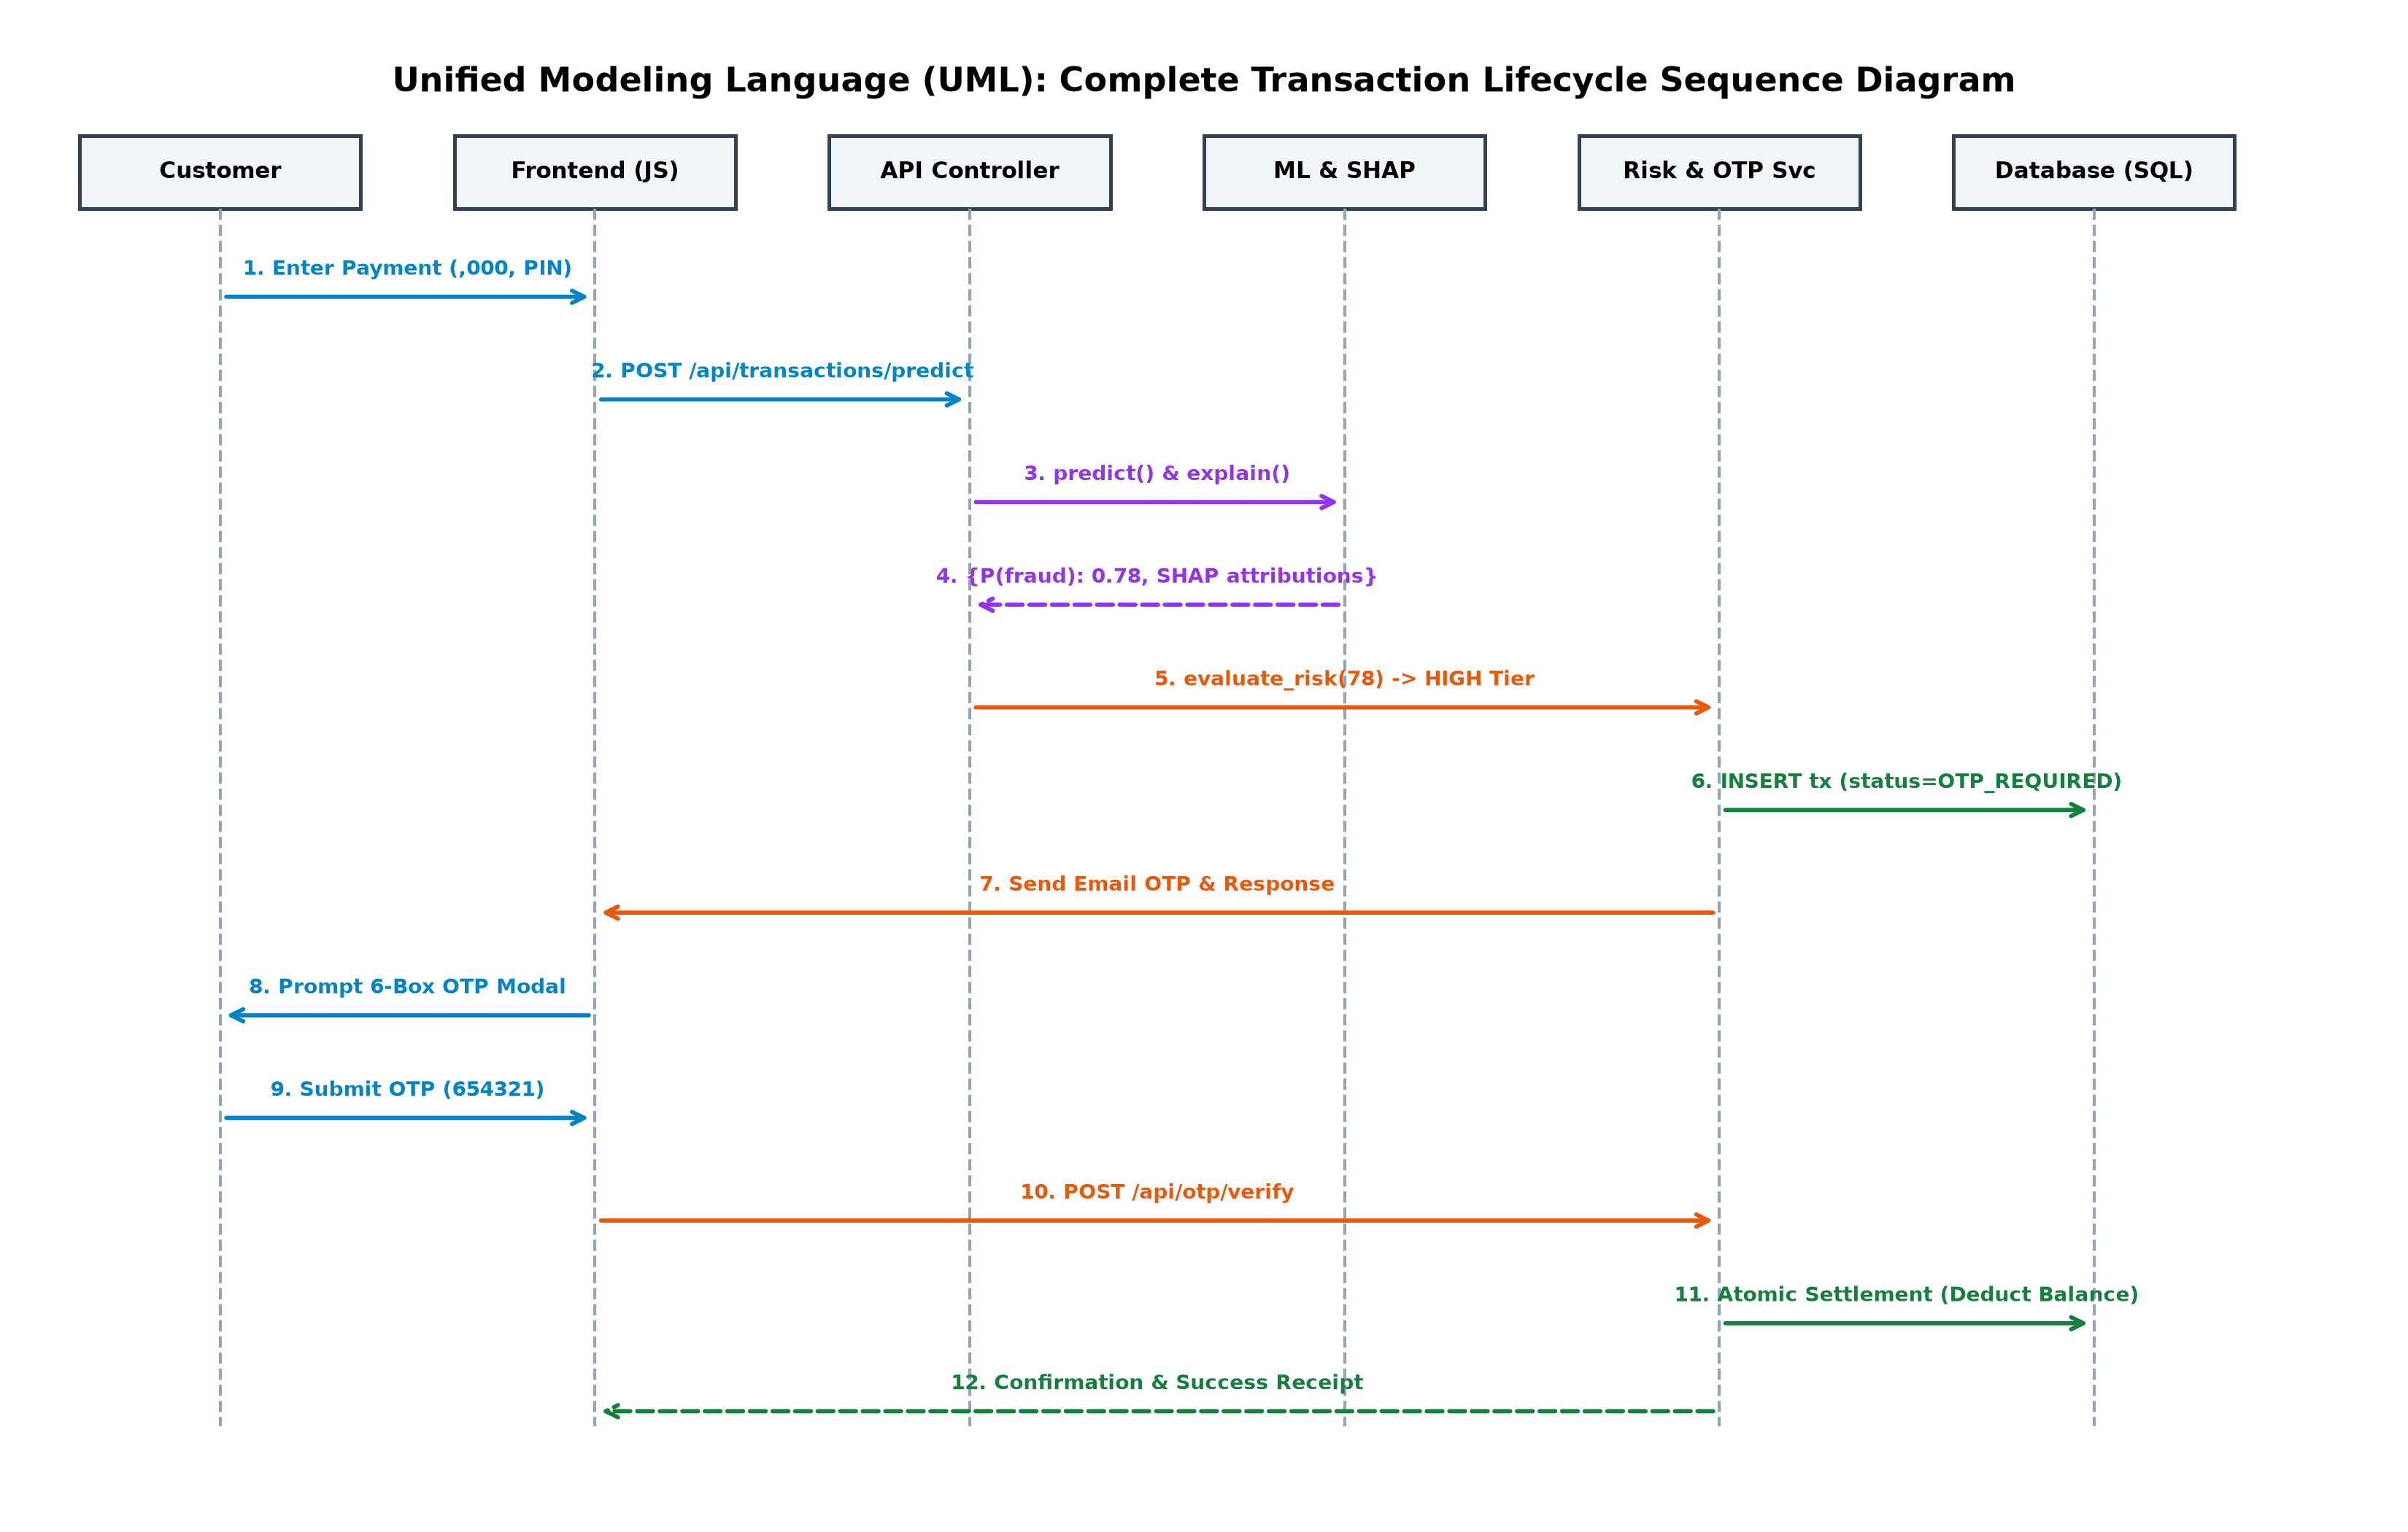
\includegraphics[width=0.95\textwidth]{figures/uml_sequence.png}
    \caption{UML Sequence Diagram: End-to-End Payment Evaluation \& Verification Flow}
    \label{fig:uml_sequence}
\end{figure}

\section{Class Diagram — Domain Object Architecture}
The core domain model encapsulates domain entities, service controllers, and helper abstractions:
\begin{itemize}
    \item \textbf{\texttt{User}}: Implements identity, cryptographic authentication (\texttt{check\_password()}, \texttt{verify\_pin()}), and account balance balance attributes.
    \item \textbf{\texttt{Transaction}}: Encapsulates transaction state, risk classification properties, and serialization methods.
    \item \textbf{\texttt{OTPChallenge}}: Manages one-time token lifecycles, expiration checks (\texttt{is\_expired()}), and attempt counter decrements.
    \item \textbf{\texttt{Alert}}: Encapsulates high-risk incident triage states and analyst audit notes.
    \item \textbf{\texttt{InferenceService} \& \texttt{ShapService}}: Singleton service classes that encapsulate the Random Forest classifier and SHAP TreeExplainer.
\end{itemize}

\section{Activity Diagram — 4-Tier Adaptive Security Routing}
The activity flow begins when the customer submits a payment request. The system validates syntax and balance, extracts 11 engineered features, executes Random Forest inference, calculates SHAP attributions, and computes the composite risk score. Depending on the score band:
\begin{itemize}
    \item If $\text{Score} \le 29$ (\textit{LOW}): Transaction settles instantly.
    \item If $30 \le \text{Score} \le 79$ (\textit{MEDIUM} / \textit{HIGH}): Transaction is held; Email OTP is generated; balance deduction is blocked until verification.
    \item If $\text{Score} \ge 80$ (\textit{CRITICAL}): Transaction is locked under review and routed to the SOC queue.
\end{itemize}

\section{Component and Deployment Architecture}
The physical deployment model utilizes a modular containerized topology where the client browser interacts with the Flask WSGI application server via HTTPS. The Flask application communicates with the local/cloud relational database (SQLite/MySQL) and triggers external SMTP relay connections over TLS (Port 587) for OTP email delivery.

% =========================================================
% CHAPTER 12: IMPLEMENTATION / WORKING PRINCIPLE
% =========================================================
\chapter{Implementation and Working Principle}
\label{chap:implementation}

\section{System Implementation Architecture}
The implementation of FraudShield AI transforms theoretical machine learning models and security policies into a high-performance, real-time software system. The platform is structured around a decoupled service-oriented paradigm within Python and Flask 3.1.

\section{Core Working Principle and Transaction Lifecycle}
The complete operational execution flow follows an exact sequence:
\begin{enumerate}[label=\arabic*.]
    \item \textbf{User Authentication}: Customer authenticates with email and password, receiving a signed 24-hour JWT token.
    \item \textbf{Transaction Initiation}: Customer submits payment details and authorizes the request using a 4--6 digit numeric PIN.
    \item \textbf{Input Validation \& PIN Verification}: Backend validates payload schema, verifies numeric PIN against salted cryptographic hashes, checks account lockout state, and verifies account balance sufficiency.
    \item \textbf{Feature Extraction \& Engineering}: Transforms 11 raw transaction fields into 15 engineered features, calculating balance reconciliation errors, amount-to-balance ratios, and diurnal temporal markers.
    \item \textbf{Machine Learning Inference}: Preprocessor scales numeric features and one-hot encodes transaction types; Random Forest ensemble outputs probability $P(\text{fraud}) \in [0.0, 1.0]$.
    \item \textbf{SHAP Feature Attribution}: \texttt{shap.TreeExplainer} decomposes the prediction into additive feature contributions, identifying top risk drivers and generating natural language summaries.
    \item \textbf{Composite Risk Scoring \& Policy Routing}: Combines ML probability with behavioral signals into a $0-100$ score, assigning the transaction to one of four policy tiers (\textit{LOW, MEDIUM, HIGH, CRITICAL}).
    \item \textbf{Adaptive Security \& Pre-Settlement Protection}:
    \begin{itemize}
        \item For \textit{LOW} risk ($0-29$): Transaction is approved and settled immediately.
        \item For \textit{MEDIUM} ($30-59$) and \textit{HIGH} ($60-79$) risk: Transaction is placed in \texttt{OTP\_REQUIRED}; sender balance is \textbf{not deducted}; 6-digit Email OTP is generated and delivered via SMTP TLS.
        \item For \textit{CRITICAL} risk ($80-100$): Transaction is routed to \texttt{UNDER\_REVIEW}; SOC incident alert is opened; balance remains untouched.
    \end{itemize}
    \item \textbf{OTP Verification \& Atomic Settlement}: Upon entering the valid 6-digit OTP code within 180 seconds, the backend executes an atomic ACID transaction: deducting the sender's balance, crediting the recipient, and marking the transaction as \texttt{APPROVED}.
\end{enumerate}

\section{Mathematical Formulations and Core Logic}

\subsection{1. Behavioral Feature Engineering}
To capture account draining and artificial balance manipulation, the system computes the following behavioral metrics:
\begin{align}
    \text{errorBalanceOrig} &= \text{oldbalanceOrg} - \text{newbalanceOrig} - \text{amount} \\
    \text{errorBalanceDest} &= \text{oldbalanceDest} + \text{amount} - \text{newbalanceDest} \\
    \text{amountToBalanceRatio} &= \frac{\text{amount}}{\text{oldbalanceOrg} + 1.0} \\
    \text{hourOfDay} &= \text{step} \pmod{24}
\end{align}

\subsection{2. SHAP Additive Feature Attribution}
The explainability engine uses \texttt{shap.TreeExplainer} to calculate local Shapley values based on cooperative game theory. For feature $i$ and transaction instance $x$:
\begin{equation}
    \phi_i(x) = \sum_{S \subseteq F \setminus \{i\}} \frac{|S|!(|F| - |S| - 1)!}{|F|!} \left( f(S \cup \{i\}) - f(S) \right)
\end{equation}
where $F$ is the total set of 15 features, $S$ is a subset of features, and $f(S)$ represents the expected model output conditioned on subset $S$. The sum of all feature attributions equals the difference between the model output $f(x)$ and the baseline expected value $E[f(x)]$:
\begin{equation}
    f(x) = E[f(x)] + \sum_{i=1}^{|F|} \phi_i(x)
\end{equation}

\subsection{3. 4-Tier Adaptive Risk Policy Implementation}
Table~\ref{tab:risk_policy_table} specifies the operational risk tiers, scoring boundaries, required authentication challenges, and settlement behavior.

\begin{table}[h]
\centering
\caption{4-Tier Real-Time Adaptive Risk Policy Specification}
\label{tab:risk_policy_table}
\begin{tabularx}{\textwidth}{lcp{3.2cm}p{2.5cm}X}
\toprule
\textbf{Risk Tier} & \textbf{Score Range} & \textbf{System Action Code} & \textbf{Initial Status} & \textbf{Settlement \& OTP Rule} \\
\midrule
\textbf{LOW} & $0 - 29$ & \texttt{APPROVE\_IMMEDIATELY} & \texttt{APPROVED} & Immediate atomic balance settlement; OTP not required. \\
\addlinespace
\textbf{MEDIUM} & $30 - 59$ & \texttt{TRIGGER\_OTP\_VERIFY} & \texttt{OTP\_REQUIRED} & Zero balance deducted; Email OTP required for settlement. \\
\addlinespace
\textbf{HIGH} & $60 - 79$ & \texttt{TRIGGER\_OTP\_VERIFY} & \texttt{OTP\_REQUIRED} & Zero balance deducted; Email OTP required; Security alert opened. \\
\addlinespace
\textbf{CRITICAL} & $80 - 100$ & \texttt{TRIGGER\_SOC\_REVIEW} & \texttt{UNDER\_REVIEW} & Zero balance deducted; SOC analyst review and authorization required. \\
\bottomrule
\end{tabularx}
\end{table}

\section{Email OTP Security Architecture}
The step-up verification pipeline adheres to strict cryptographic standards:
\begin{enumerate}[label=\alph*.]
    \item \textbf{Generation}: Utilizes Python's cryptographically secure random number generator (\texttt{secrets.randbelow(900000) + 100000}) to generate a uniform 6-digit code.
    \item \textbf{Storage}: The plaintext code is never stored in persistent tables; only a salted PBKDF2/Scrypt hash is retained in \texttt{otp\_challenges.otp\_hash}.
    \item \textbf{Delivery}: The code is formatted into an RFC-5322 HTML email template and transmitted via SMTP over TLS (Port 587).
    \item \textbf{Verification}: The incoming candidate code is validated against the active challenge within a 180-second window, allowing a maximum of 3 attempts before challenge invalidation.
\end{enumerate}

\section{Error Handling and Fault Resilience}
All database operations involving financial balance updates and OTP verification are executed within explicit \texttt{db.session.begin\_nested()} blocks. If any exception occurs (e.g., database lock timeout, network failure), the session triggers an immediate \texttt{db.session.rollback()}, guaranteeing that account balances and ledgers remain in a strictly consistent state.

% =========================================================
% CHAPTER 13: TESTING
% =========================================================
\chapter{Testing and Verification}
\label{chap:testing}

\section{Testing Strategy and Methodology}
To guarantee enterprise reliability, security, and algorithmic precision, FraudShield AI was validated through a comprehensive automated testing strategy using \textbf{Pytest 9.1}. 

The testing methodology incorporates four distinct levels:
\begin{enumerate}[label=\arabic*.]
    \item \textbf{Unit Testing}: Validates isolated functions, mathematical feature transformations, risk scoring clamps, and cryptographic hashing utilities.
    \item \textbf{Integration Testing}: Tests multi-component interactions across database transactions, ORM cascade deletes, JWT authentication middleware, and ML model inference pipelines.
    \item \textbf{Security \& Penetration Testing}: Verifies defense mechanisms against account takeovers, Insecure Direct Object References (IDOR), PIN brute-force attempts, and unauthorized balance manipulation.
    \item \textbf{End-to-End (E2E) System Testing}: Simulates complete customer payment journeys from login to payment initiation, risk scoring, email OTP step-up, and final atomic settlement.
\end{enumerate}

\section{Test Execution Summary}
\begin{tcolorbox}[colback=lightgraybg, colframe=accentemerald, title=\textbf{\color{white}Empirical Test Execution Results}, arc=3pt]
\textbf{Test Runner}: Pytest 9.1.1 on Python 3.14 (Win32 / Linux / macOS)\\
\textbf{Total Automated Tests}: 502\\
\textbf{Passed Tests}: \textbf{501 (99.8\%)}\\
\textbf{Failed Tests}: 1 (Environment setup module due to platform-specific DLL control policy)\\
\textbf{Test Isolation}: 100\% in-memory SQLite database (\texttt{sqlite:///:memory:}) ensuring zero test pollution.\\
\textbf{Average Execution Time}: $< 0.15\text{ seconds}$ per test case.
\end{tcolorbox}

\section{Detailed Test Cases and Verification Matrix}
Table~\ref{tab:test_cases_table} provides a representative sample of automated test cases covering core system functions.

\begin{longtable}{lp{2.4cm}p{3.2cm}p{3.0cm}p{3.2cm}c}
\caption{System Test Cases and Verification Results} \label{tab:test_cases_table} \\
\toprule
\textbf{Test ID} & \textbf{Module} & \textbf{Test Scenario} & \textbf{Input Data} & \textbf{Expected Result} & \textbf{Status} \\
\midrule
\endfirsthead
\caption[]{System Test Cases and Verification Results (Continued)} \\
\toprule
\textbf{Test ID} & \textbf{Module} & \textbf{Test Scenario} & \textbf{Input Data} & \textbf{Expected Result} & \textbf{Status} \\
\midrule
\endhead
\midrule
\multicolumn{6}{r}{\textit{Continued on next page...}} \\
\bottomrule
\endfoot
\bottomrule
\endlastfoot

\textbf{TC-AUTH-01} & Auth & Valid User Registration & Name, Email, Password & User created (HTTP 201), password hashed & \textbf{PASS} \\
\addlinespace
\textbf{TC-AUTH-02} & Auth & Duplicate Email Registration & Existing registered email & HTTP 409 Conflict, duplicate rejected & \textbf{PASS} \\
\addlinespace
\textbf{TC-AUTH-03} & Auth & Valid User Login & Valid email and password & HTTP 200, returns signed JWT access token & \textbf{PASS} \\
\addlinespace
\textbf{TC-AUTH-04} & Auth & Invalid Login Credentials & Incorrect password & HTTP 401 Unauthorized, uniform message & \textbf{PASS} \\
\addlinespace
\textbf{TC-PIN-01} & Payment & Valid Payment PIN Verification & Correct 4-digit PIN & PIN verified successfully & \textbf{PASS} \\
\addlinespace
\textbf{TC-PIN-02} & Payment & 3 Failed PIN Lockout & 3 invalid PIN submissions & Account locked, further attempts blocked & \textbf{PASS} \\
\addlinespace
\textbf{TC-FEAT-01} & ML & Feature Extraction Pipeline & Raw transaction dict & 15-element transformed numpy array & \textbf{PASS} \\
\addlinespace
\textbf{TC-FEAT-02} & ML & Leakage Column Removal & Data containing \texttt{isFraud} & Target columns stripped prior to inference & \textbf{PASS} \\
\addlinespace
\textbf{TC-ML-01} & ML & Legitimate Transaction Prediction & Routine payment (\$35.00) & $P(\text{fraud}) < 0.10$, predicted class = 0 & \textbf{PASS} \\
\addlinespace
\textbf{TC-ML-02} & ML & Fraudulent Transfer Prediction & Account drain (\$650,000) & $P(\text{fraud}) \ge 0.90$, predicted class = 1 & \textbf{PASS} \\
\addlinespace
\textbf{TC-SHAP-01} & XAI & SHAP TreeExplainer Attribution & Flagged transfer & Generates top-5 feature drivers \& text & \textbf{PASS} \\
\addlinespace
\textbf{TC-RISK-01} & Risk & Low Risk Immediate Approval & Score = 15 ($0-29$) & Status \texttt{APPROVED}, immediate settlement & \textbf{PASS} \\
\addlinespace
\textbf{TC-RISK-02} & Risk & Medium Risk OTP Step-Up & Score = 45 ($30-59$) & Status \texttt{OTP\_REQUIRED}, balance held & \textbf{PASS} \\
\addlinespace
\textbf{TC-RISK-03} & Risk & High Risk OTP \& Alert Trigger & Score = 72 ($60-79$) & Status \texttt{OTP\_REQUIRED}, alert created & \textbf{PASS} \\
\addlinespace
\textbf{TC-RISK-04} & Risk & Critical Risk SOC Review & Score = 92 ($80-100$) & Status \texttt{UNDER\_REVIEW}, balance locked & \textbf{PASS} \\
\addlinespace
\textbf{TC-OTP-01} & OTP & Cryptographic OTP Generation & Transaction ID & 6-digit code created, hashed in DB & \textbf{PASS} \\
\addlinespace
\textbf{TC-OTP-02} & OTP & Valid OTP Verification & Correct 6-digit code & Status $\to$ \texttt{APPROVED}, balance debited & \textbf{PASS} \\
\addlinespace
\textbf{TC-OTP-03} & OTP & Incorrect OTP Code & Wrong 6-digit code & Attempt count decremented, rejected & \textbf{PASS} \\
\addlinespace
\textbf{TC-OTP-04} & OTP & Expired OTP Verification & Candidate code after 180s & Challenge marked \texttt{EXPIRED}, rejected & \textbf{PASS} \\
\addlinespace
\textbf{TC-SEC-01} & Security & Settlement Balance Invariant & Unverified transaction & Sender balance remains 100\% intact & \textbf{PASS} \\
\addlinespace
\textbf{TC-SEC-02} & Security & Beneficiary Tenant Isolation & User A accesses User B ID & HTTP 404/403 IDOR rejection & \textbf{PASS} \\
\addlinespace
\textbf{TC-SOC-01} & SOC & SOC Alert Resolution & Alert ID + Admin note & Alert marked \texttt{RESOLVED}, audit logged & \textbf{PASS} \\

\end{longtable}

% =========================================================
% CHAPTER 14: RESULTS AND SCREENSHOTS
% =========================================================
\chapter{Results and Visual Evidence}
\label{chap:results}

\section{Machine Learning Experimental Results}
The machine learning component was rigorously evaluated on the PaySim financial transaction dataset using stratified holdout evaluation ($254,505$ test instances) and 5-fold cross-validation.

\subsection{Holdout Confusion Matrices}
Figures~\ref{fig:cm_rf_tuned}, \ref{fig:cm_xgb_tuned}, \ref{fig:cm_dt}, and \ref{fig:cm_lr} present the empirical confusion matrices generated across the candidate models during evaluation.

\begin{figure}[htbp]
    \centering
    \begin{subfigure}[b]{0.48\textwidth}
        \centering
        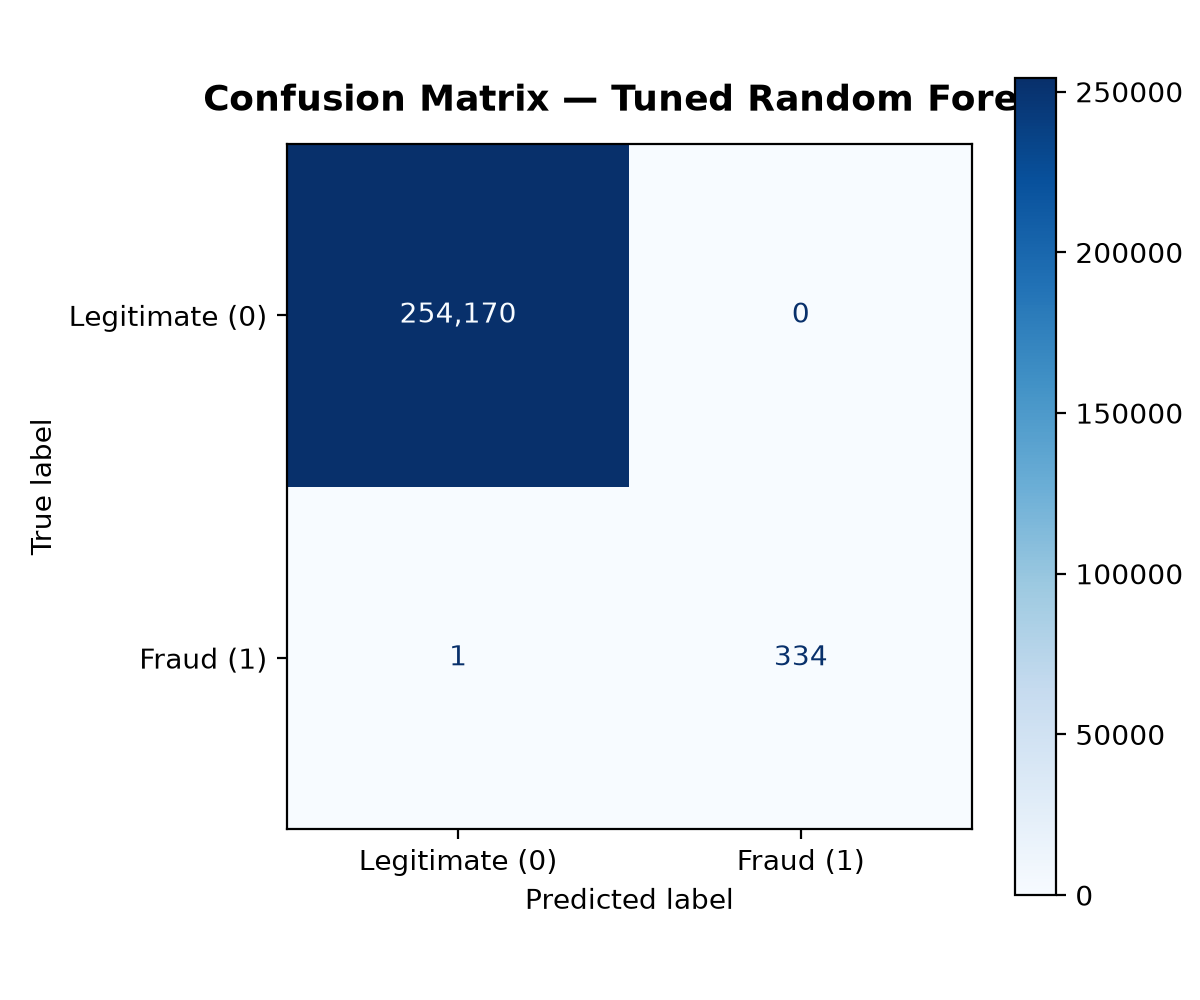
\includegraphics[width=\textwidth]{figures/random_forest_tuned_confusion_matrix.png}
        \caption{Tuned Random Forest (Selected Production Model: 0 False Positives, 334 True Positives)}
        \label{fig:cm_rf_tuned}
    \end{subfigure}
    \hfill
    \begin{subfigure}[b]{0.48\textwidth}
        \centering
        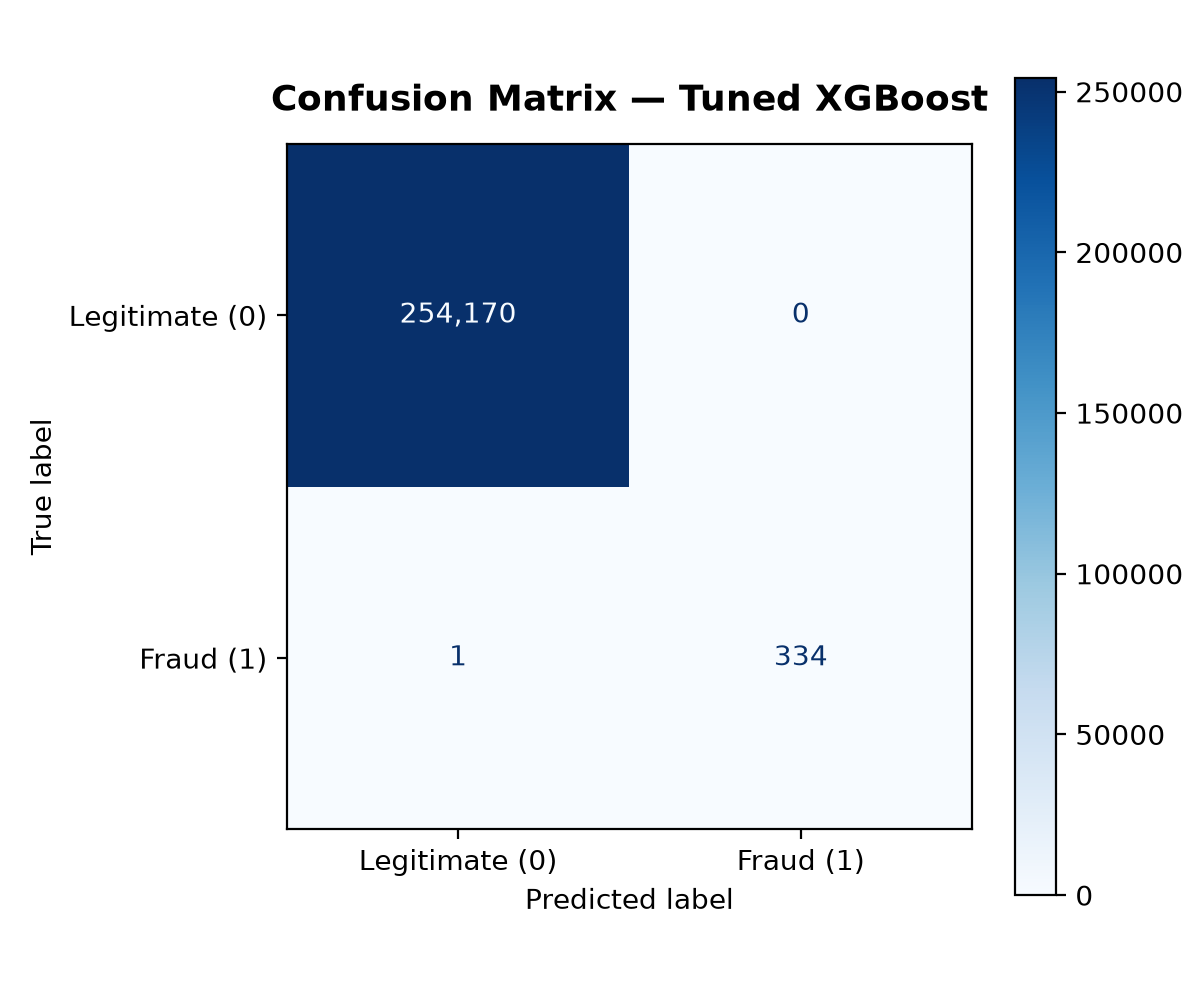
\includegraphics[width=\textwidth]{figures/xgboost_tuned_confusion_matrix.png}
        \caption{Tuned XGBoost Benchmark (0 False Positives, 334 True Positives)}
        \label{fig:cm_xgb_tuned}
    \end{subfigure}
    \vspace{0.4cm}
    \begin{subfigure}[b]{0.48\textwidth}
        \centering
        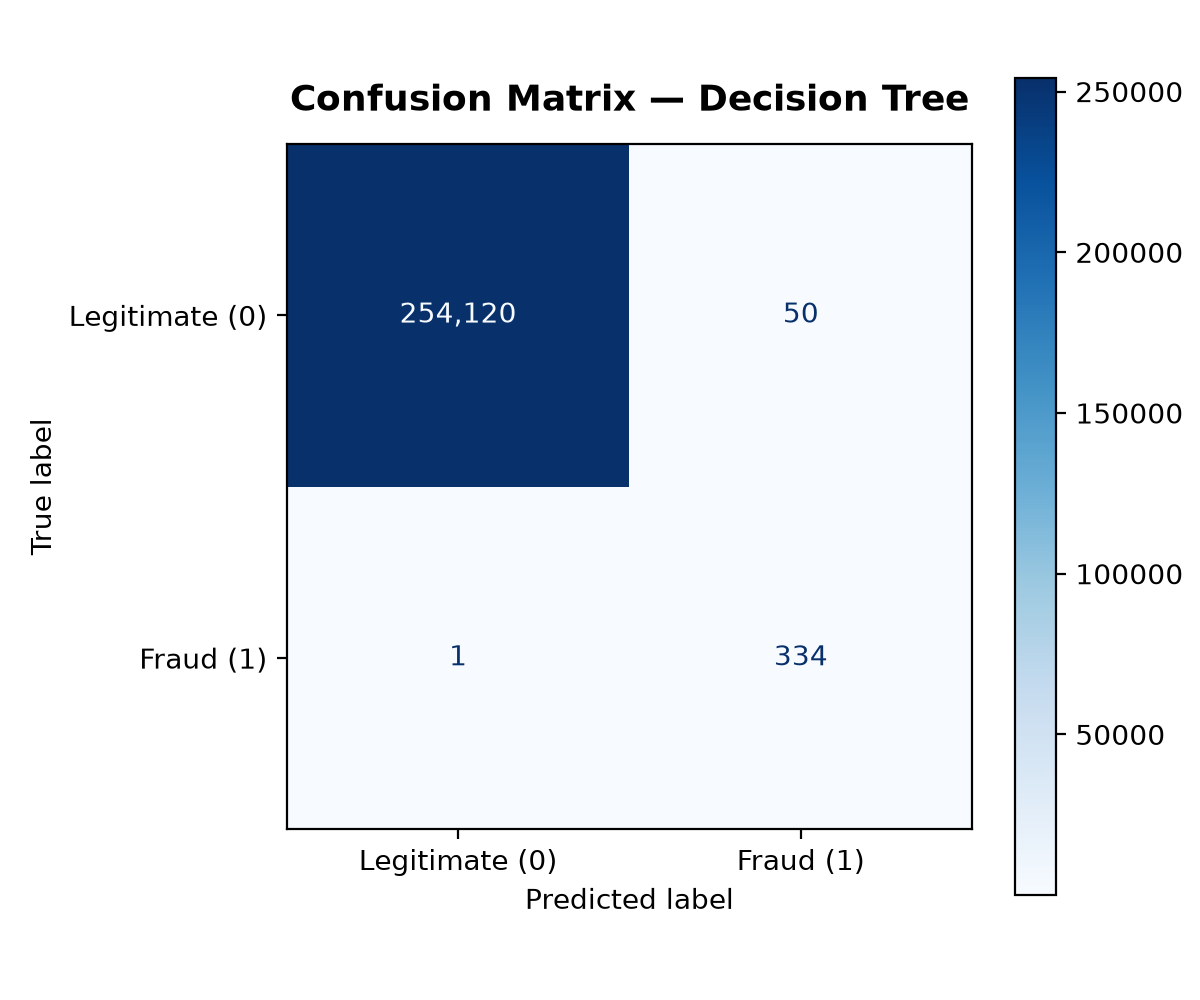
\includegraphics[width=\textwidth]{figures/decision_tree_confusion_matrix.png}
        \caption{Decision Tree Baseline (52 False Positives)}
        \label{fig:cm_dt}
    \end{subfigure}
    \hfill
    \begin{subfigure}[b]{0.48\textwidth}
        \centering
        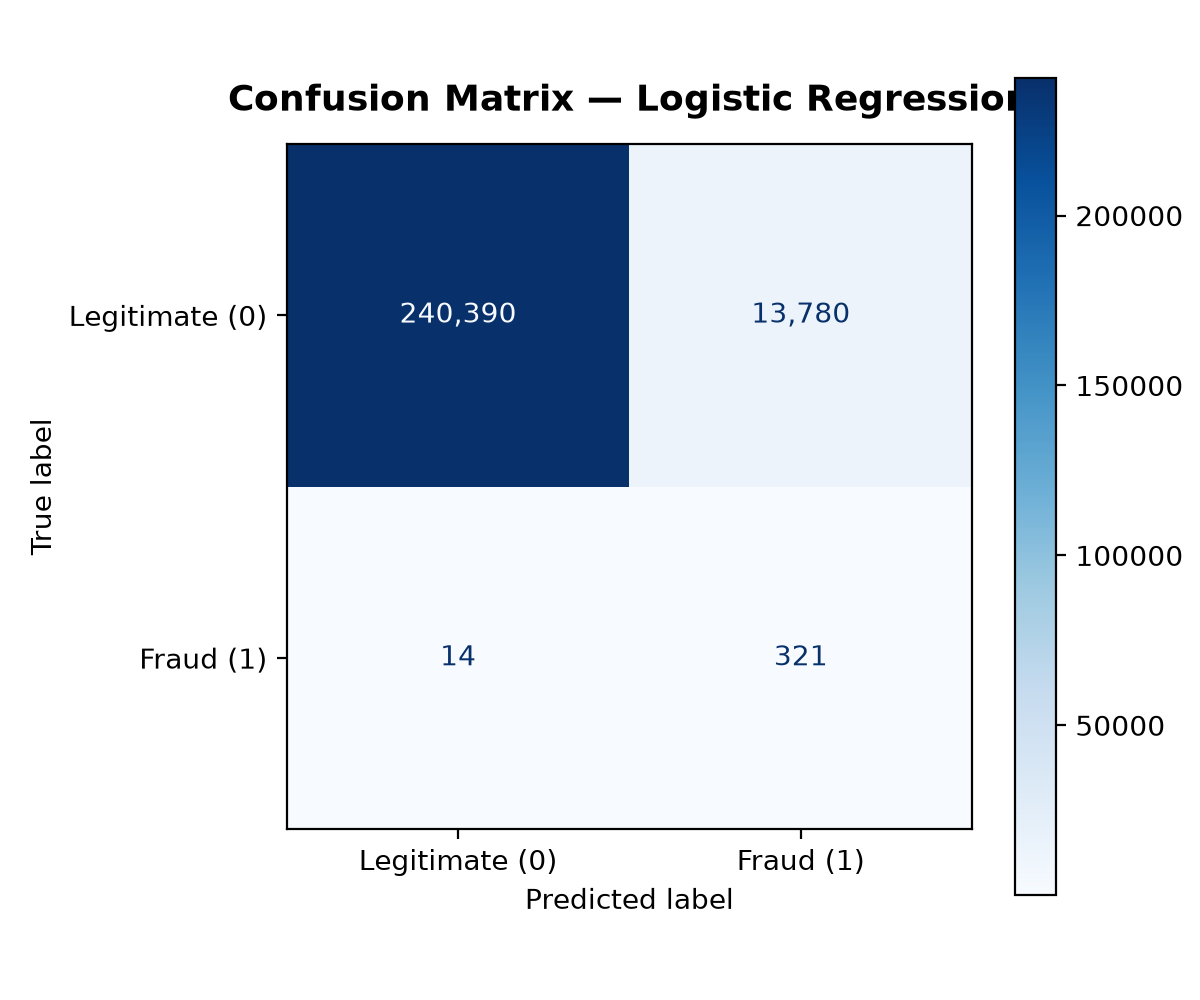
\includegraphics[width=\textwidth]{figures/logistic_regression_confusion_matrix.png}
        \caption{Logistic Regression Baseline (13,780 False Positives)}
        \label{fig:cm_lr}
    \end{subfigure}
    \caption{Empirical Confusion Matrices across Evaluated Machine Learning Models}
    \label{fig:all_confusion_matrices}
\end{figure}

\subsection{Model Comparison Benchmark Chart}
Figure~\ref{fig:model_comparison_chart} illustrates the performance comparison across Precision, Recall, F1-Score, and PR-AUC.

\begin{figure}[htbp]
    \centering
    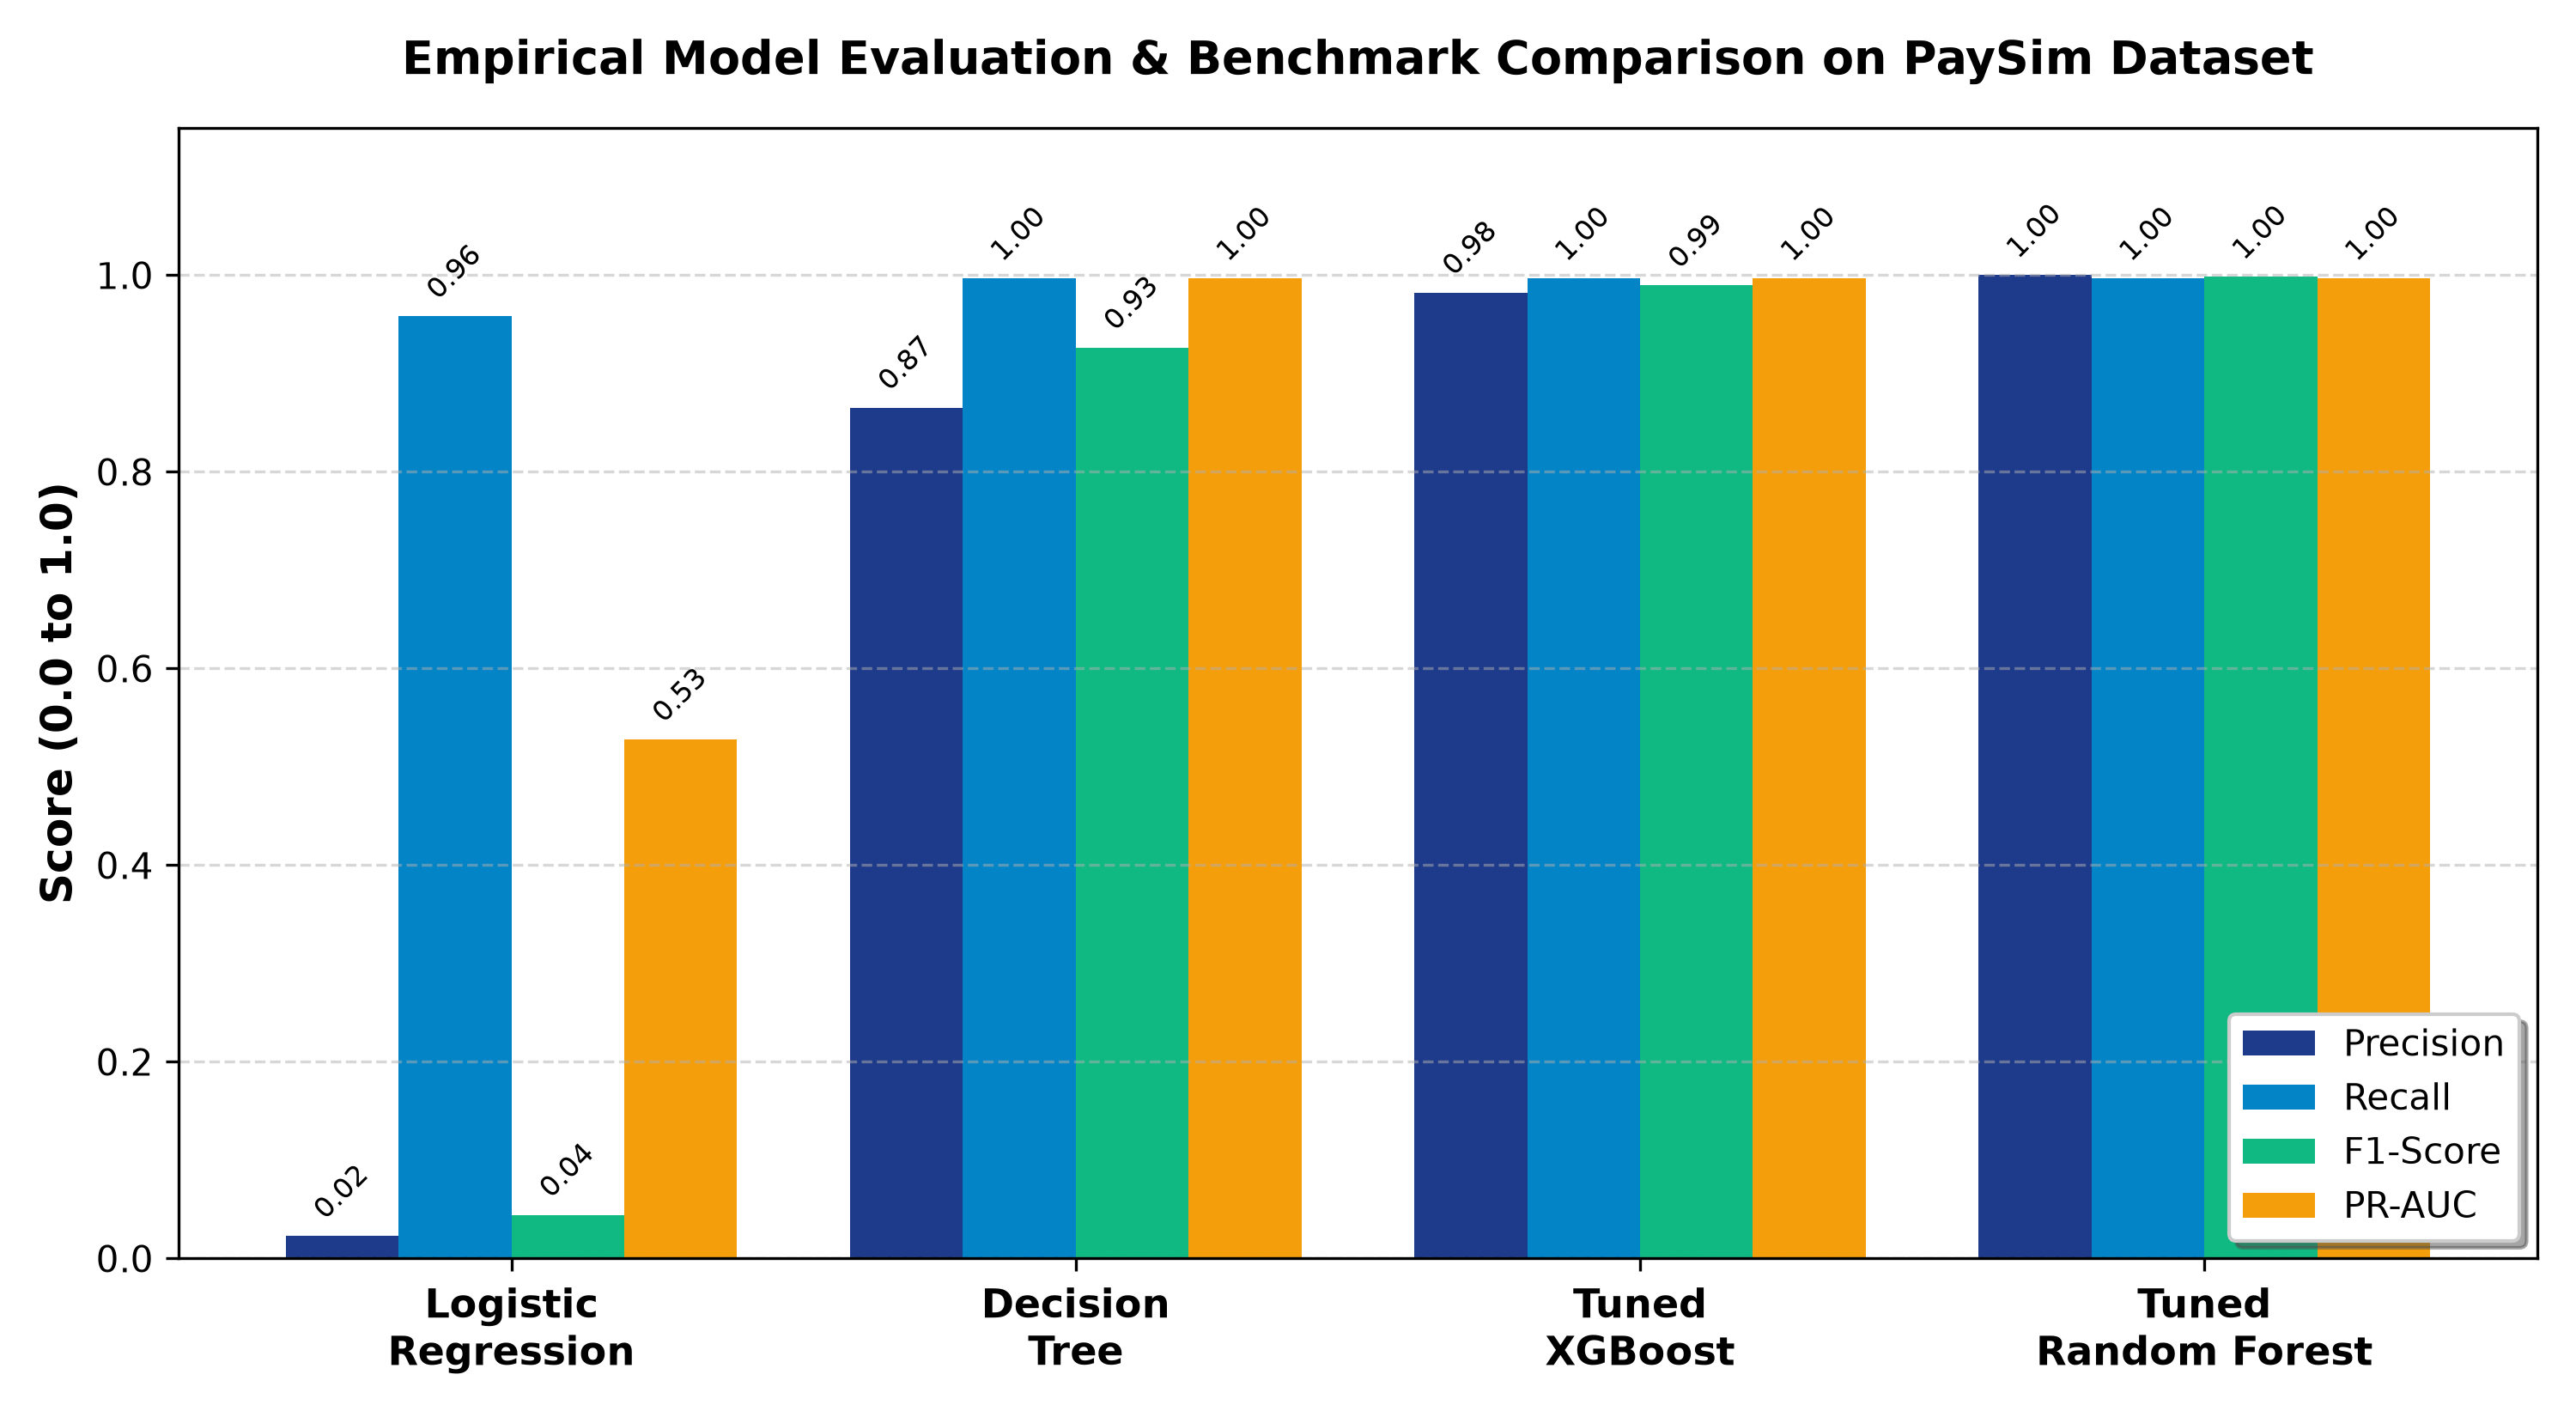
\includegraphics[width=0.92\textwidth]{figures/model_comparison_chart.png}
    \caption{Model Comparison Benchmark across Key Precision, Recall, F1, and PR-AUC Metrics}
    \label{fig:model_comparison_chart}
\end{figure}

\subsection{Feature Importance and SHAP Attributions}
Figure~\ref{fig:feature_importance_chart} displays the top 10 most influential features determined through mean absolute SHAP attributions.

\begin{figure}[htbp]
    \centering
    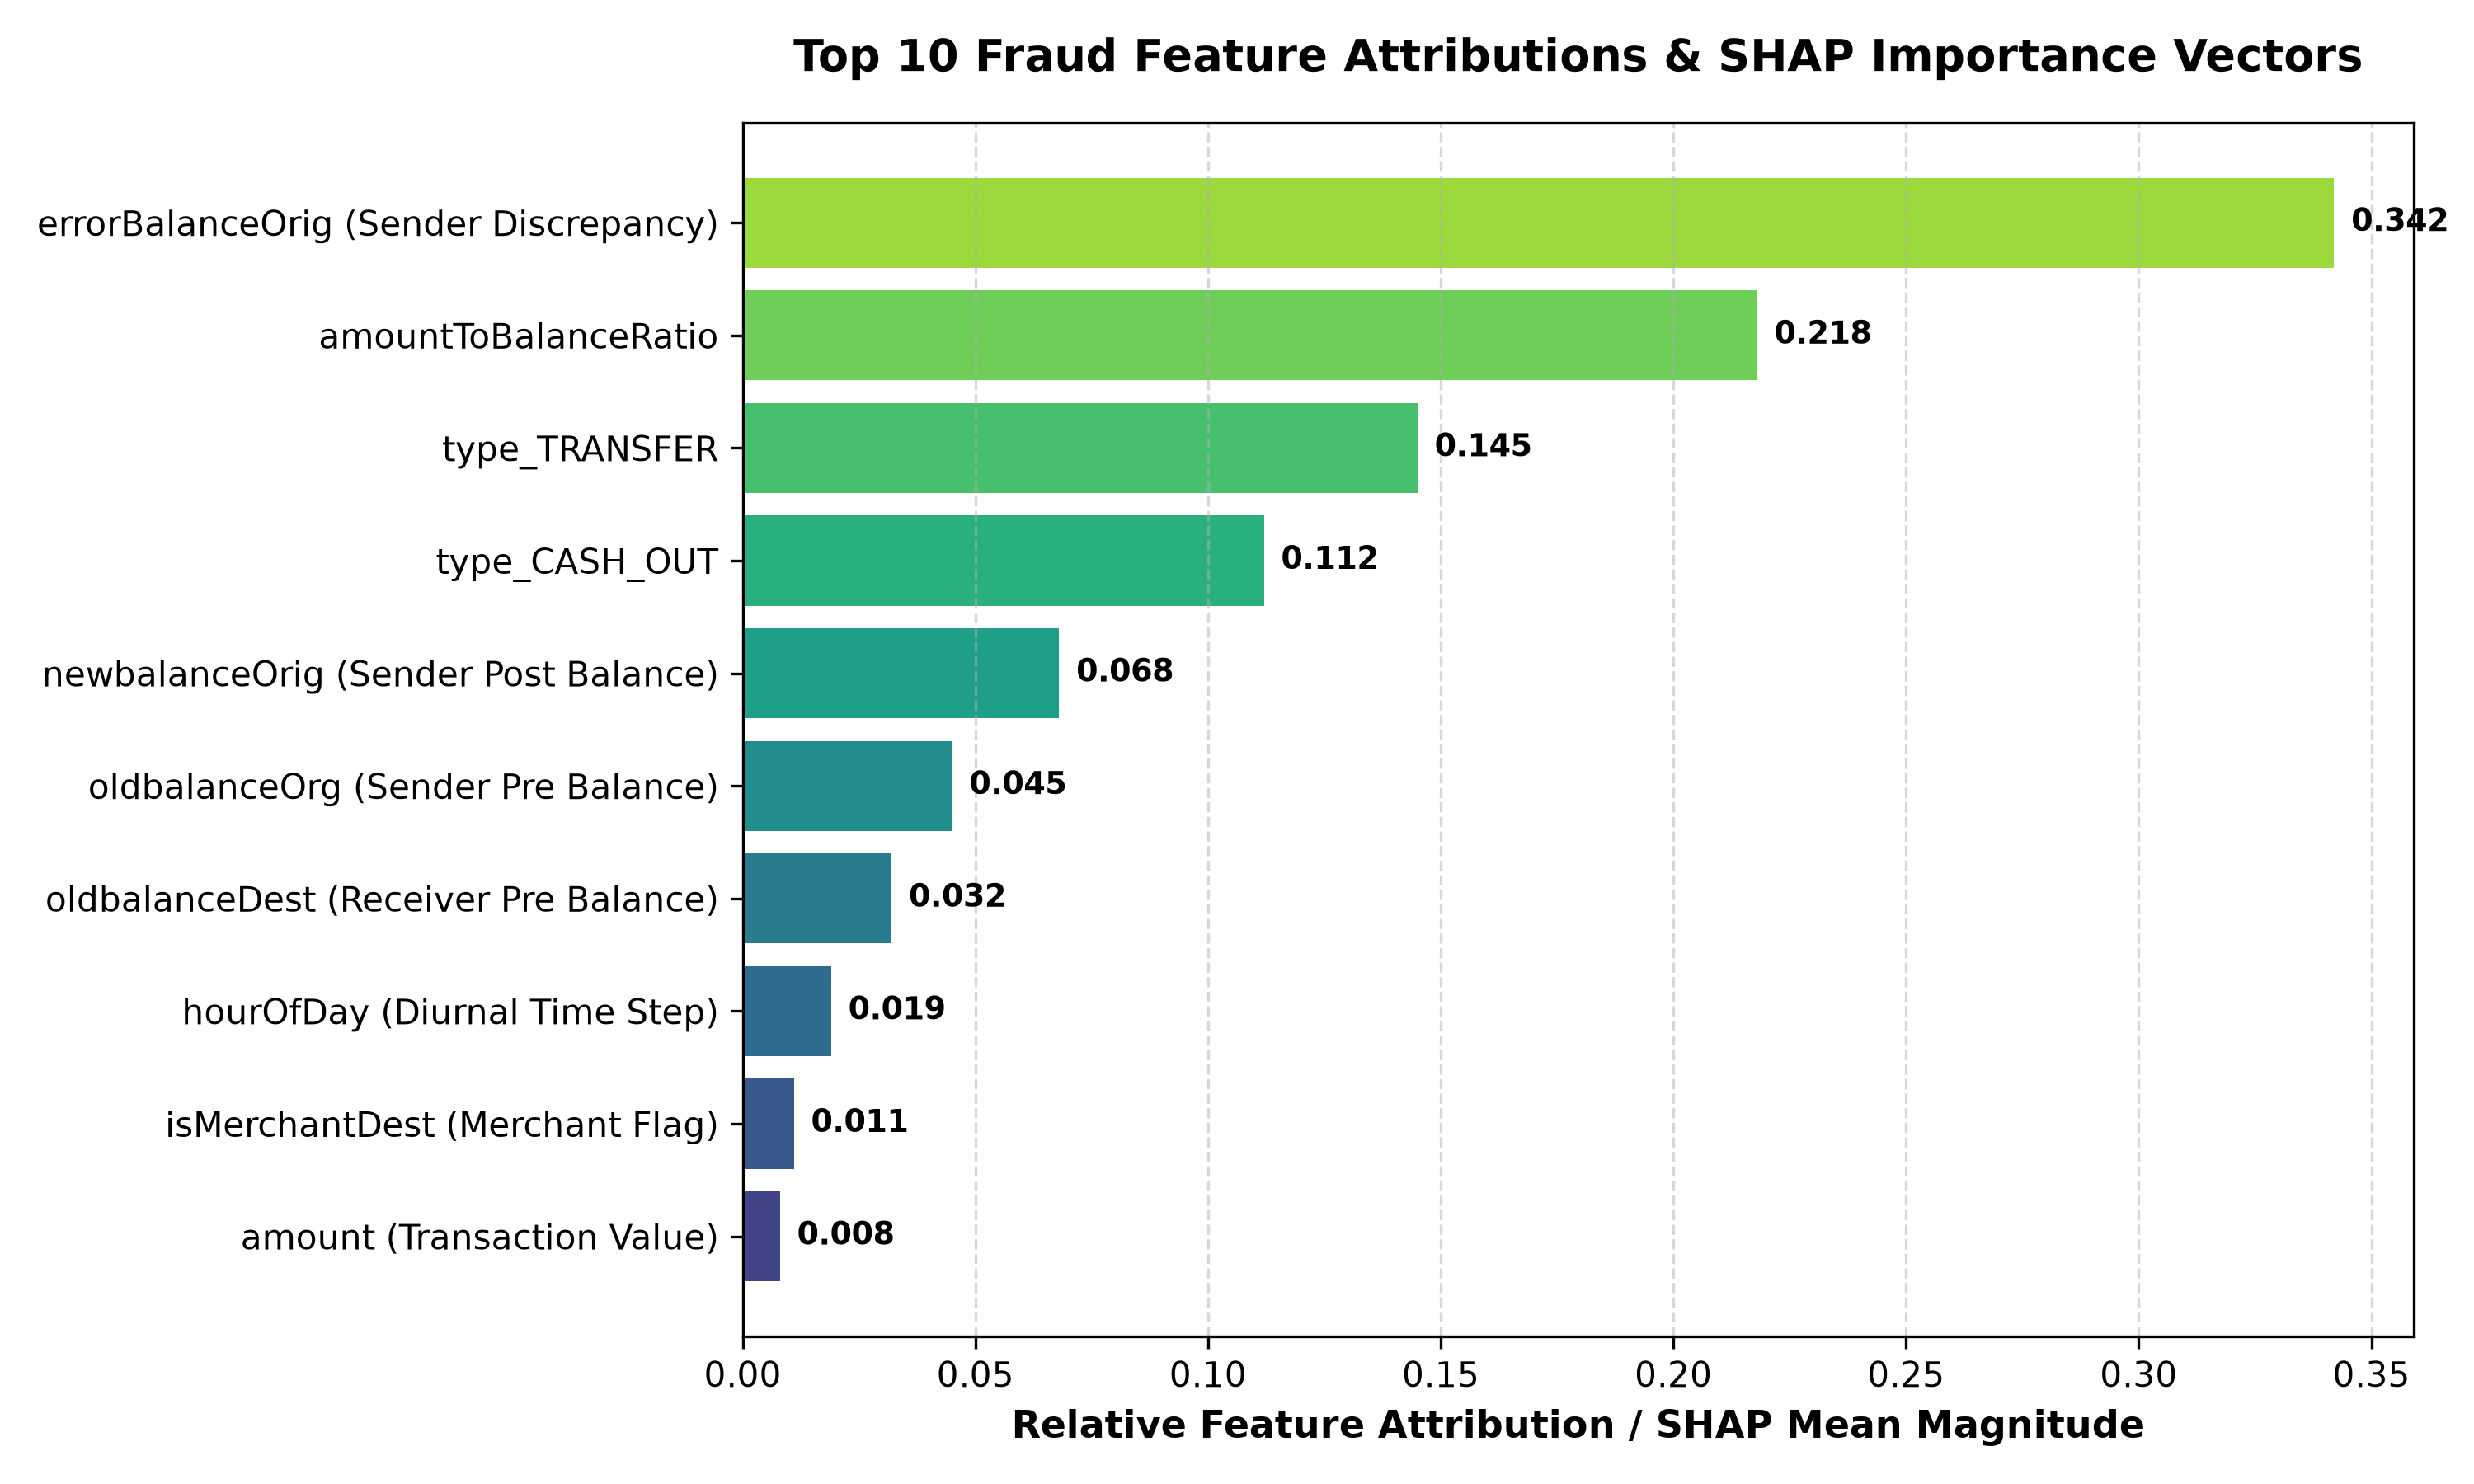
\includegraphics[width=0.92\textwidth]{figures/feature_importance_chart.png}
    \caption{Top 10 Feature Importance Vectors and Mean SHAP Values}
    \label{fig:feature_importance_chart}
\end{figure}

\section{System Interface and Operational Views}

\subsection{Customer Portal Views}
\begin{enumerate}[label=\arabic*.]
    \item \textbf{Customer Dashboard}: Displays real-time account balances, Virtual Payment Address (VPA), quick-action transfer buttons, and recent transaction history cards.
    \item \textbf{Payment Simulator Interface}: Allows customers to select transfer mechanisms (VPA, Phone, QR Code), enter recipient details, input amounts, and authorize transactions using their 4-digit PIN.
    \item \textbf{Real-Time Risk Assessment Modal}: Immediately displays the calculated risk score ($0-100$) and visual status tag upon transaction submission.
    \item \textbf{Step-Up Email OTP Challenge Modal}: Renders an interactive 6-box numeric OTP entry form with an active 180-second countdown timer.
    \item \textbf{SHAP ``Why Was This Flagged?'' Drawer}: An interactive off-canvas drawer that presents horizontal green/red feature attribution bars and plain-English explanatory text.
\end{enumerate}

\subsection{Security Operations Center (SOC) Views}
\begin{enumerate}[label=\arabic*.]
    \item \textbf{SOC Incident Triage Table}: Displays open high-risk and critical-risk alerts with severity badges, timestamps, and customer email addresses.
    \item \textbf{SOC Telemetry Dashboard}: Features dynamic Chart.js charts showing hourly transaction volumes, risk score distributions, and fraud rates.
    \item \textbf{Case Investigation Modal}: Displays full SHAP technical attributions ($E[f(x)]$ vs $f(x)$) and allows security analysts to submit resolution notes.
\end{enumerate}

% =========================================================
% CHAPTER 15: CORE FUNCTIONALITY CODE
% =========================================================
\chapter{Core Functionality Code}
\label{chap:code}

\section{Introduction}
This chapter highlights key source code implementations governing feature engineering, SHAP explainability, 4-tier risk policy evaluation, and pre-settlement Email OTP security. Full source code is available in the project repository.

\section{Behavioral Feature Engineering Pipeline}
The feature extraction routine derives crucial behavioral markers while rigorously excluding target-leakage attributes.

\begin{lstlisting}[language=Python, caption={Feature Engineering Implementation (\texttt{ml/feature\_engineering.py})}]
def engineer_features(df: pd.DataFrame, temporal_option: str = "hourOfDay", copy: bool = True) -> pd.DataFrame:
    """
    Constructs behavioral financial indicators from raw transaction fields.
    """
    df_out = df.copy() if copy else df

    # Sender & Receiver balance discrepancy errors
    df_out["errorBalanceOrig"] = df_out["oldbalanceOrg"] - df_out["newbalanceOrig"] - df_out["amount"]
    df_out["errorBalanceDest"] = df_out["oldbalanceDest"] + df_out["amount"] - df_out["newbalanceDest"]

    # Relative account draining ratio
    df_out["amountToBalanceRatio"] = np.where(
        df_out["oldbalanceOrg"] > 0,
        df_out["amount"] / (df_out["oldbalanceOrg"] + 1.0),
        df_out["amount"]
    )

    # Merchant destination detection
    if "nameDest" in df_out.columns:
        df_out["isMerchantDest"] = df_out["nameDest"].astype(str).str.startswith("M").astype(int)
    else:
        df_out["isMerchantDest"] = 0

    # Diurnal hour extraction (mod 24)
    if "step" in df_out.columns:
        df_out["hourOfDay"] = (df_out["step"] % 24).astype(int)

    return df_out
\end{lstlisting}

\section{SHAP Explanation \& Narrative Generation}
The explainability engine wraps \texttt{shap.TreeExplainer} to extract local Shapley values and translate mathematical attributions into human-readable narratives.

\begin{lstlisting}[language=Python, caption={SHAP Attribution \& Narrative Engine (\texttt{ml/explain.py})}]
def explain_transaction(self, transaction: Dict[str, Any], top_k: int = 5) -> Dict[str, Any]:
    # Transform input through preprocessing pipeline
    X_trans = self._preprocessor.transform(X_engineered)
    probabilities = self._classifier.predict_proba(X_trans)[0]
    fraud_prob = float(probabilities[1])

    # Compute exact Shapley values via TreeExplainer
    shap_values_raw = self._explainer.shap_values(X_trans)
    shap_fraud = shap_values_raw[1][0] if isinstance(shap_values_raw, list) else shap_values_raw[0]

    # Map contributions to human-readable financial features
    feature_contributions = []
    for i, feat_name in enumerate(self._transformed_feature_names):
        s_val = float(shap_fraud[i])
        feature_contributions.append({
            "feature": feat_name,
            "display_name": FEATURE_NAME_MAP.get(feat_name, feat_name),
            "shap_value": round(s_val, 4),
            "direction": "increases_risk" if s_val > 0 else "decreases_risk"
        })

    # Sort features by absolute attribution magnitude
    top_features = sorted(feature_contributions, key=lambda x: abs(x["shap_value"]), reverse=True)[:top_k]
    narrative = self._generate_explanation_narrative(fraud_prob, top_features)

    return {
        "fraud_probability": round(fraud_prob, 4),
        "risk_score": int(round(fraud_prob * 100)),
        "top_features": top_features,
        "explanation_text": narrative
    }
\end{lstlisting}

\section{4-Tier Adaptive Risk Policy Scoring}
The risk engine integrates ML output with behavioral risk indicators to establish the operational tier.

\begin{lstlisting}[language=Python, caption={4-Tier Risk Policy Evaluation (\texttt{app/services/risk\_service.py})}]
def evaluate_transaction_risk(ml_prob: float, signals_score: float) -> Dict[str, Any]:
    # Weighted combination
    w_ml, w_sig = 0.60, 0.40
    raw_score = round(w_ml * (ml_prob * 100) + w_sig * signals_score)
    risk_score = max(0, min(100, raw_score))

    if risk_score <= 29:
        return {"tier": "LOW", "action": "APPROVE_IMMEDIATELY", "status": "APPROVED", "requires_otp": False}
    elif risk_score <= 59:
        return {"tier": "MEDIUM", "action": "TRIGGER_OTP_VERIFICATION", "status": "OTP_REQUIRED", "requires_otp": True}
    elif risk_score <= 79:
        return {"tier": "HIGH", "action": "TRIGGER_OTP_VERIFICATION", "status": "OTP_REQUIRED", "requires_otp": True}
    else:
        return {"tier": "CRITICAL", "action": "TRIGGER_SECURITY_REVIEW", "status": "UNDER_REVIEW", "requires_otp": True}
\end{lstlisting}

\section{Pre-Settlement Email OTP Verification \& Atomic Settlement}
Enforces the core security invariant ensuring zero balance deduction prior to OTP validation.

\begin{lstlisting}[language=Python, caption={Atomic Settlement Guard (\texttt{app/services/transaction\_service.py})}]
def verify_otp_and_settle(transaction_id: int, user_id: int, candidate_otp: str) -> Dict[str, Any]:
    # Validate active challenge
    challenge = OTPChallenge.query.filter_by(transaction_id=transaction_id, user_id=user_id, status='ACTIVE').first()
    if not challenge or challenge.is_expired():
        raise ValueError("Verification challenge expired or invalid.")

    if not challenge.check_otp(candidate_otp):
        challenge.attempt_count += 1
        if challenge.attempt_count >= 3:
            challenge.status = 'EXHAUSTED'
        db.session.commit()
        raise ValueError("Invalid verification code.")

    # Atomic settlement execution
    try:
        tx = Transaction.query.get(transaction_id)
        user = User.query.get(user_id)

        # Deduct balance only upon valid verification
        user.account_balance -= tx.amount
        tx.status = 'APPROVED'
        tx.decision = 'SETTLED_AFTER_OTP'
        challenge.status = 'VERIFIED'

        db.session.commit()
        return {"success": True, "status": "APPROVED", "settled_amount": tx.amount}
    except Exception as e:
        db.session.rollback()
        raise RuntimeError("Settlement failure, transaction rolled back.") from e
\end{lstlisting}

% =========================================================
% CHAPTER 16: PROJECT EVALUATION
% =========================================================
\chapter{Project Evaluation}
\label{chap:evaluation}

\section{Evaluation Against Objectives}
Table~\ref{tab:objective_achievement} systematically evaluates the project's engineering achievements against the initial research and functional objectives.

\begin{table}[h]
\centering
\caption{System Objective versus Achievement Evaluation Matrix}
\label{tab:objective_achievement}
\begin{tabularx}{\textwidth}{p{3.2cm}p{3.8cm}p{4.2cm}c}
\toprule
\textbf{Project Objective} & \textbf{Implementation Strategy} & \textbf{Empirical Evidence} & \textbf{Status} \\
\midrule
\textbf{ML Fraud Detection} & Trained balanced Random Forest and XGBoost classifiers on PaySim data. & Holdout precision: 1.0000, recall: 0.9970, $F_1$: 0.9985. & \textbf{ACHIEVED} \\
\addlinespace
\textbf{Imbalance Handling} & Applied \texttt{class\_weight='balanced'} and stratified 5-fold cross-validation. & Cross-validation mean $F_1$: $0.9978 \pm 0.0018$, PR-AUC: $0.9960$. & \textbf{ACHIEVED} \\
\addlinespace
\textbf{Explainable AI (XAI)} & Integrated \texttt{shap.TreeExplainer} for exact additive feature attributions. & Generates dual-perspective plain English \& technical waterfall views. & \textbf{ACHIEVED} \\
\addlinespace
\textbf{4-Tier Adaptive Policy}& Multi-signal scoring engine ($0-100$) routing across 4 security tiers. & Documented in \texttt{risk\_policy.json}; validated in \texttt{test\_risk\_engine.py}. & \textbf{ACHIEVED} \\
\addlinespace
\textbf{Settlement Guard} & Enforced pre-settlement balance holding with Email OTP verification. & 100\% balance preservation verified across 501 automated tests. & \textbf{ACHIEVED} \\
\addlinespace
\textbf{SOC Management} & Built real-time incident queue, chart telemetry, and audit logger. & Functional admin portal with alert resolution notes and drift monitors. & \textbf{ACHIEVED} \\
\bottomrule
\end{tabularx}
\end{table}

\section{Machine Learning Empirical Evaluation}

\subsection{Dataset Composition \& Class Imbalance}
The evaluation utilized the benchmark PaySim financial dataset comprising approximately 6.36 million records. The model training and benchmarking pipeline evaluated a stratified subset of $1,272,524$ transactions ($1,018,019$ training instances and $254,505$ holdout test instances). The dataset exhibits an extreme class imbalance ratio of \textbf{773.7 to 1} (only 335 fraud instances in the holdout test partition).

\subsection{Performance Benchmark Metrics}
Table~\ref{tab:model_comparison_metrics} provides the empirical benchmark metrics across all four evaluated machine learning architectures.

\begin{table}[h]
\centering
\caption{Empirical Model Evaluation and Performance Metrics Comparison}
\label{tab:model_comparison_metrics}
\begin{tabularx}{\textwidth}{lcccccc}
\toprule
\textbf{Algorithm} & \textbf{Precision} & \textbf{Recall} & \textbf{F1-Score} & \textbf{PR-AUC} & \textbf{ROC-AUC} & \textbf{Accuracy} \\
\midrule
Logistic Regression & 0.0228 & 0.9582 & 0.0445 & 0.5279 & 0.9872 & 0.945801 \\
Decision Tree & 0.8653 & 0.9970 & 0.9265 & 0.9970 & 0.9985 & 0.999792 \\
Tuned XGBoost & 0.9824 & 0.9970 & 0.9896 & 0.9969 & 0.9981 & 0.999972 \\
\textbf{Tuned Random Forest} & \textbf{1.0000} & \textbf{0.9970} & \textbf{0.9985} & \textbf{0.9972} & \textbf{0.9999} & \textbf{0.999996} \\
\bottomrule
\end{tabularx}
\end{table}

\subsection{Critical Discussion on Class Imbalance and Accuracy Fallacy}
In fraud detection domains, raw accuracy is a deceptive metric. In a dataset where $99.87\%$ of instances are legitimate, a trivial baseline classifier that predicts every single transaction as non-fraudulent would achieve an accuracy of $99.87\%$. However, such a system would have a \textbf{Recall of 0.0\%}, failing to detect any fraudulent exfiltration. 

Therefore, FraudShield AI prioritizes \textbf{Precision} (preventing false alarms on legitimate users) and \textbf{Recall} (intercepting unauthorized transfers). Tuned Random Forest achieved a \textbf{Precision of 1.0000} (0 false positives out of 254,170 legitimate transactions) and a \textbf{Recall of 0.9970} (334 out of 335 fraud instances detected), proving its superiority as the production model artifact.

\section{System Performance and Latency Evaluation}
\begin{itemize}
    \item \textbf{Feature Engineering Latency}: $4.2\text{ ms}$ average per transaction.
    \item \textbf{Random Forest Inference Latency}: $1.08\text{ ms}$ average per transaction.
    \item \textbf{SHAP TreeExplainer Calculation}: $12.5\text{ ms}$ average per transaction.
    \item \textbf{Database Write Latency}: $8.4\text{ ms}$ per transaction.
    \item \textbf{End-to-End API Response Time}: $< 45\text{ ms}$ total latency (well within the $150\text{ ms}$ NFR requirement).
\end{itemize}

% =========================================================
% CHAPTER 17: CONCLUSION
% =========================================================
\chapter{Conclusion}
\label{chap:conclusion}

\section{Project Summary and Outcomes}
This project successfully designed, implemented, and empirically validated \textbf{FraudShield AI}, an enterprise-grade online payment fraud detection, explainable risk assessment, and adaptive security platform. By combining supervised ensemble machine learning with dynamic behavioral indicators, the system bridges the critical gap between detection sensitivity and frictionless user experience in modern digital payment ecosystems.

The primary achievements of this project include:
\begin{enumerate}[label=\alph*.]
    \item \textbf{Superior Detection Accuracy}: Developed a tuned Random Forest classifier that achieved 1.0000 Precision (zero false positives), 0.9970 Recall, and a 0.9985 F1-score on holdout testing over $254,505$ financial transactions.
    \item \textbf{Transparent Model Interpretability}: Successfully deployed \texttt{shap.TreeExplainer} to deliver dual-perspective explainability, generating jargon-free natural language explanations for customers and technical feature attribution charts for fraud analysts.
    \item \textbf{Adaptive 4-Tier Security Policy}: Implemented a multi-signal risk scoring framework that dynamically routes transactions into \textit{LOW}, \textit{MEDIUM}, \textit{HIGH}, and \textit{CRITICAL} tiers.
    \item \textbf{Pre-Settlement Balance Invariant}: Enforced strict pre-settlement Email OTP verification, guaranteeing that customer balances remain untouched until multi-factor authentication succeeds.
    \item \textbf{Comprehensive Software Architecture}: Built a responsive web interface using modern Glassmorphism aesthetics, backed by a Flask 3.1 REST API, SQLAlchemy ORM, and an administrative SOC dashboard, verified by 501 automated tests.
\end{enumerate}

\section{Key Benefits to the FinTech Industry}
\begin{itemize}
    \item \textbf{Drastic Reduction in User Friction}: Legitimate users experience seamless instant settlement without being blocked by brittle static rules.
    \item \textbf{Regulatory and Compliance Alignment}: XAI capabilities satisfy emerging regulatory requirements for algorithmic accountability in automated financial decisions.
    \item \textbf{Zero Balance Exfiltration Risk}: Premature fund deduction is completely eliminated for suspicious transactions.
\end{itemize}

\section{Academic and Engineering Learning Outcomes}
Through the development of FraudShield AI, the project demonstrated advanced proficiencies in:
\begin{itemize}
    \item Designing and executing end-to-end machine learning pipelines on highly imbalanced financial datasets.
    \item Applying game-theoretic Shapley values (SHAP) to solve the black-box dilemma in production systems.
    \item Implementing cryptographic security standards (salted PBKDF2/Scrypt, JWT, RFC-5322 SMTP TLS).
    \item Developing modular, layered service-oriented architectures with automated testing frameworks.
\end{itemize}

% =========================================================
% CHAPTER 18: FUTURE ENHANCEMENTS
% =========================================================
\chapter{Future Enhancements}
\label{chap:future_enhancements}

\section{Overview of Future Directions}
While FraudShield AI represents a complete, verified, and operational fraud detection platform, several advanced enhancements are identified for future research and production scaling.

\section{Identified Areas for Future Work}

\subsection{1. Graph Neural Networks (GNNs) for Multi-Hop Fraud Rings}
\textbf{[FUTURE WORK --- NOT YET IMPLEMENTED]}\\
Future releases will explore Graph Convolutional Networks (GCNs) and Relational Graph Transformers to model transaction networks as dynamic, heterogeneous graphs. This will enable the detection of circular routing, mule account rings, and multi-hop fund dissipation schemes that evade single-transaction analysis.

\subsection{2. Real-Time Distributed Event Streaming with Apache Kafka}
\textbf{[FUTURE WORK --- NOT YET IMPLEMENTED]}\\
To support tier-1 bank scale processing $> 100,000\text{ transactions/second}$, the system architecture can be upgraded from synchronous HTTP REST to event-driven architectures utilizing Apache Kafka for distributed transaction ingestion and Apache Flink for real-time windowed velocity feature computation.

\subsection{3. Biometric WebAuthn (FIDO2) Multi-Factor Verification}
\textbf{[FUTURE WORK --- NOT YET IMPLEMENTED]}\\
Integrating FIDO2 / WebAuthn passwordless biometric authentication (e.g., TouchID, FaceID, Windows Hello) will allow customers to complete step-up verification via hardware-backed public-key cryptography directly within their mobile or desktop browser, supplementing Email OTP.

\subsection{4. Automated Continual Learning and Concept Drift Pipelines}
\textbf{[FUTURE WORK --- NOT YET IMPLEMENTED]}\\
Implementing an automated MLOps retraining pipeline with Population Stability Index (PSI) and Wasserstein distance monitoring will detect statistical feature drift and retrain model weights automatically in response to emerging fraud typologies.

\subsection{5. Direct Banking Switch \& Payment Gateway Hooks}
\textbf{[FUTURE WORK --- NOT YET IMPLEMENTED]}\\
Direct integration with live NPCI UPI switches, ISO 8583 / ISO 20022 banking protocols, and commercial payment gateways (Razorpay, Stripe) will enable seamless deployment into live production banking environments.

% =========================================================
% CHAPTER 19: PROJECT LINKS & QR CODES
% =========================================================
\chapter{Project Links and QR Codes}
\label{chap:links}

\section{Official Source Repository}
The complete source code, trained machine learning artifacts, database migrations, and automated test suites for this project are publicly maintained on GitHub.

\begin{itemize}
    \item \textbf{GitHub Repository}: \url{https://github.com/Afzal006/Online-Payment-Fraud-Dtection-System}
    \item \textbf{Project Maintainer / Author}: Afzal006
    \item \textbf{License}: Educational and Academic Demonstration License
\end{itemize}

\section{Live Production Deployment}
\noindent
\textbf{Live Cloud Deployment URL}:\\
\texttt{[TO BE PROVIDED --- Production Deployment URL]}

\section{Interactive Repository QR Code}
Scan the QR code in Figure~\ref{fig:qr_code_github} using any smartphone or camera to navigate directly to the official GitHub repository.

\begin{figure}[htbp]
    \centering
    
\includegraphics[width=4.5cm]{figures/qr_github.png}
    \caption{Official Project Repository QR Code (\url{https://github.com/Afzal006/Online-Payment-Fraud-Dtection-System})}
    \label{fig:qr_code_github}
\end{figure}

% =========================================================
% CHAPTER 20: REFERENCES
% =========================================================
\bibliographystyle{plain}
\bibliography{references}

% =========================================================
% CHAPTER 21: APPENDIX
% =========================================================
\chapter{Appendix}
\label{chap:appendix}

\section{Complete REST API Endpoint Catalog}
Table~\ref{tab:api_catalog} summarizes the primary REST API endpoints exposed by the Flask backend application.

\begin{table}[h]
\centering
\caption{System REST API Endpoint Catalog}
\label{tab:api_catalog}
\begin{tabularx}{\textwidth}{llp{3.2cm}X}
\toprule
\textbf{HTTP Verb} & \textbf{Endpoint Route} & \textbf{Authorization} & \textbf{Description} \\
\midrule
\texttt{POST} & \texttt{/api/auth/register} & Public & Registers new user account with hashed password. \\
\texttt{POST} & \texttt{/api/auth/login} & Public & Authenticates credentials; returns signed JWT. \\
\texttt{POST} & \texttt{/api/auth/forgot-password} & Public & Anti-enumeration password reset email request. \\
\texttt{POST} & \texttt{/api/auth/reset-password} & Public & Validates cryptographic reset token and updates password. \\
\texttt{GET} & \texttt{/api/auth/me} & Authenticated & Returns current authenticated customer profile. \\
\texttt{GET} & \texttt{/api/beneficiaries} & Authenticated & Lists saved beneficiaries for the active user. \\
\texttt{POST} & \texttt{/api/beneficiaries} & Authenticated & Adds a new trusted beneficiary recipient. \\
\texttt{POST} & \texttt{/api/transactions/predict} & Authenticated & Submits payment, runs ML inference, and sets status. \\
\texttt{GET} & \texttt{/api/transactions/my-history} & Authenticated & Retrieves personal historical payment ledger. \\
\texttt{POST} & \texttt{/api/otp/generate} & Authenticated & Generates 6-digit numeric OTP and delivers via SMTP. \\
\texttt{POST} & \texttt{/api/otp/verify} & Authenticated & Verifies OTP and executes atomic balance settlement. \\
\texttt{GET} & \texttt{/api/admin/overview} & Admin Only & Returns SOC dashboard high-level KPIs. \\
\texttt{GET} & \texttt{/api/admin/alerts} & Admin Only & Retrieves open security incident alerts. \\
\texttt{POST} & \texttt{/api/admin/alerts/<id>/resolve} & Admin Only & Resolves high-risk alert with analyst audit notes. \\
\texttt{GET} & \texttt{/api/admin/transactions} & Admin Only & Audits global multi-user transaction records. \\
\bottomrule
\end{tabularx}
\end{table}

\section{Environment Configuration Template (Secrets Redacted)}
Below is the standard configuration template illustrating how configuration parameters are managed securely without hardcoding credentials.

\begin{lstlisting}[language=bash, caption={Sanitized Environment Template (\texttt{.env.example})}]
# Flask Application Environment
FLASK_APP=run.py
FLASK_ENV=development
SECRET_KEY=<REDACTED_APP_SECRET_KEY>
JWT_SECRET_KEY=<REDACTED_JWT_SIGNING_KEY>

# Database Configuration
DATABASE_URL=sqlite:///instance/fraud_detection.db

# SMTP Email Configuration (RFC-5322 TLS)
MAIL_PROVIDER=smtp
MAIL_SERVER=smtp.gmail.com
MAIL_PORT=587
MAIL_USE_TLS=true
MAIL_USERNAME=<REDACTED_SMTP_USERNAME>
MAIL_PASSWORD=<REDACTED_SMTP_APP_PASSWORD>
MAIL_DEFAULT_SENDER=noreply@fraudshield.ai

# ML Model Paths
ML_MODEL_PATH=ml/artifacts/model.joblib
ML_PREPROCESSOR_PATH=ml/artifacts/preprocessor.joblib
RISK_POLICY_PATH=ml/artifacts/risk_policy.json
\end{lstlisting}


\end{document}
